%% ============================================================
%% MIVA-KNIGHT: Comprehensive Unified Thesis
%% Multimodal Interactive Voice Assistant with
%% Knowledge-driven Hybrid Intelligence and Adaptive Domain Transfer
%% Author: Oluwakayode (Kayode) Soyinka
%% IT 581 Capstone — Concordia University of Edmonton
%% Supervisor: Dr. Baidya Saha
%% ============================================================
\documentclass[12pt,a4paper]{article}

%% ── Encoding & Fonts ────────────────────────────────────────
\usepackage[utf8]{inputenc}
\usepackage[T1]{fontenc}
\usepackage[expansion=false]{microtype}

%% ── Page Geometry ───────────────────────────────────────────
\usepackage[margin=2.5cm,top=3cm,bottom=3cm,headheight=14pt]{geometry}

%% ── Mathematics ─────────────────────────────────────────────
\usepackage{amsmath,amssymb,amsthm,mathtools}
\usepackage{bm}

%% ── Algorithms ──────────────────────────────────────────────
\usepackage{algorithm}
\usepackage{algpseudocode}
\usepackage{algorithmicx}
\algnewcommand\algorithmicforeach{\textbf{for each}}
\algdef{S}[FOR]{ForEach}[1]{\algorithmicforeach\ #1\ \textbf{do}}
\algnewcommand\algorithmicInput{\textbf{Input:}}
\algnewcommand\algorithmicOutput{\textbf{Output:}}
\algnewcommand\INPUT{\item[\algorithmicInput]}
\algnewcommand\OUTPUT{\item[\algorithmicOutput]}
\renewcommand{\algorithmicrequire}{\textbf{Require:}}
\renewcommand{\algorithmicensure}{\textbf{Ensure:}}

%% ── TikZ & Drawing ──────────────────────────────────────────
\usepackage{tikz}
\usetikzlibrary{
  shapes.geometric, shapes.misc,
  arrows.meta, arrows,
  positioning, fit, calc,
  backgrounds, patterns,
  decorations.pathreplacing,
  decorations.markings,
  matrix, chains, shadows
}
\usepackage{pgfplots}
\pgfplotsset{compat=1.18}

%% ── Scaling & Resize ────────────────────────────────────────
\usepackage{graphicx}
\usepackage{adjustbox}
\usepackage{float}
\usepackage{caption}
\usepackage{subcaption}

%% ── Tables ──────────────────────────────────────────────────
\usepackage{booktabs}
\usepackage{tabularx}
\usepackage{longtable}
\usepackage{multirow}
\usepackage{colortbl}
\usepackage{array}

%% ── Colours ─────────────────────────────────────────────────
\usepackage[dvipsnames,svgnames,table]{xcolor}

%% ── Boxes ───────────────────────────────────────────────────
\usepackage{tcolorbox}
\tcbuselibrary{breakable,skins,theorems}

%% ── Typography ──────────────────────────────────────────────
\usepackage{setspace}
\onehalfspacing
\usepackage{parskip}
\usepackage{enumitem}
\usepackage{titlesec}

%% ── Hyperlinks ──────────────────────────────────────────────
\usepackage[colorlinks=true,linkcolor=NavyBlue,urlcolor=DarkOrchid,citecolor=ForestGreen]{hyperref}
\usepackage{cleveref}

%% ── Headers / Footers ───────────────────────────────────────
\usepackage{fancyhdr}
\pagestyle{fancy}
\fancyhf{}
\fancyhead[L]{\small\textsc{MIVA-KNIGHT: Comprehensive Thesis}}
\fancyhead[R]{\small\textsc{Soyinka — IT 581}}
\fancyfoot[C]{\thepage}
\renewcommand{\headrulewidth}{0.4pt}

%% ── Bibliography ────────────────────────────────────────────
\usepackage[numbers]{natbib}
\usepackage{url}

%% ── Section Formatting ──────────────────────────────────────
\titleformat{\section}{\Large\bfseries\color{NavyBlue}}{\thesection}{1em}{}[\titlerule]
\titleformat{\subsection}{\large\bfseries\color{MidnightBlue}}{\thesubsection}{1em}{}
\titleformat{\subsubsection}{\normalsize\bfseries\color{RoyalBlue}}{\thesubsubsection}{1em}{}

%% ── Colour Palette ──────────────────────────────────────────
\definecolor{navyblue}{RGB}{20,60,120}
\definecolor{midblue}{RGB}{60,120,190}
\definecolor{coralred}{RGB}{210,80,70}
\definecolor{mintgreen}{RGB}{60,160,110}
\definecolor{amber}{RGB}{200,140,30}
\definecolor{lavender}{RGB}{120,90,170}
\definecolor{deepteal}{RGB}{20,100,100}
\definecolor{boxblue}{RGB}{210,225,245}
\definecolor{boxred}{RGB}{245,215,215}
\definecolor{boxorange}{RGB}{255,232,205}
\definecolor{boxgray}{RGB}{228,228,228}
\definecolor{boxgreen}{RGB}{200,235,210}
\definecolor{boxpurple}{RGB}{228,215,242}
\definecolor{lightblue}{RGB}{220,235,255}
\definecolor{lightgreen}{RGB}{220,245,230}
\definecolor{lossred}{RGB}{190,30,30}
\definecolor{cDark}{RGB}{40,60,100}
\definecolor{cPhase1}{RGB}{200,225,255}
\definecolor{cPhase2}{RGB}{255,220,200}
\definecolor{cPhase3}{RGB}{210,245,215}
\definecolor{encodercolor}{RGB}{60,120,200}
\definecolor{fusioncolor}{RGB}{200,80,20}
% RL-specific
\definecolor{robotblue}{RGB}{30,90,160}
\definecolor{rlgreen}{RGB}{20,140,60}
\definecolor{rlred}{RGB}{180,40,40}
\definecolor{memorycol}{RGB}{200,180,240}
\definecolor{qnetcol}{RGB}{170,210,250}
\definecolor{actioncol}{RGB}{245,220,170}
\definecolor{nlpcol}{RGB}{200,240,200}
% Challenge-specific
\definecolor{reprYellow}{RGB}{255,252,210}
\definecolor{reprBorder}{RGB}{200,190,100}
\definecolor{fuseRose}{RGB}{255,225,230}
\definecolor{fuseBorder}{RGB}{200,140,150}
\definecolor{coLearnPurple}{RGB}{235,225,255}
\definecolor{coLearnBorder}{RGB}{150,120,200}
\definecolor{alignBlue}{RGB}{210,235,255}
\definecolor{alignBorder}{RGB}{100,140,200}
\definecolor{transGray}{RGB}{240,240,240}
\definecolor{transBorder}{RGB}{130,130,130}
\definecolor{modalA}{RGB}{30,80,160}
\definecolor{modalB}{RGB}{180,40,40}

%% ── Theorem Environments ────────────────────────────────────
\theoremstyle{definition}
\newtheorem{definition}{Definition}[section]
\newtheorem{axiom}{Axiom}[section]
\newtheorem{example}{Example}[section]

\theoremstyle{plain}
\newtheorem{theorem}{Theorem}[section]
\newtheorem{lemma}[theorem]{Lemma}
\newtheorem{corollary}[theorem]{Corollary}
\newtheorem{proposition}[theorem]{Proposition}

\theoremstyle{remark}
\newtheorem{remark}{Remark}[section]

%% ── TikZ Node Styles (Global) ───────────────────────────────
\tikzset{
  basebox/.style={rectangle,rounded corners=4pt,draw=black!55,align=center,font=\small},
  inputnode/.style={basebox,fill=cDark,text=white,minimum width=2.8cm,minimum height=1.0cm,font=\small\bfseries},
  encnode/.style={basebox,fill=boxblue,draw=navyblue!70,minimum width=3.2cm,minimum height=1.0cm,thick},
  projnode/.style={basebox,fill=boxorange,draw=amber!70,minimum width=3.2cm,minimum height=1.0cm,thick},
  retnode/.style={basebox,fill=boxgreen,draw=mintgreen!70,minimum width=3.2cm,minimum height=1.0cm},
  gennode/.style={basebox,fill=boxred,draw=coralred!70,minimum width=3.2cm,minimum height=1.0cm},
  outnode/.style={basebox,fill=boxpurple,draw=lavender!70,minimum width=3.0cm,minimum height=0.9cm},
  lossnode/.style={basebox,fill=boxorange,draw=amber!80,minimum width=3.2cm,minimum height=1.0cm},
  datanode/.style={basebox,fill=boxgray,minimum width=2.8cm,minimum height=0.9cm},
  decnode/.style={diamond,draw=amber!90,fill=yellow!20,aspect=2.5,align=center,font=\small\bfseries,minimum width=2.8cm,minimum height=1.2cm},
  qnetnode/.style={basebox,fill=qnetcol,draw=robotblue,minimum width=3.0cm,minimum height=2.0cm,thick},
  memnode/.style={basebox,fill=memorycol,draw=lavender,minimum width=3.0cm,minimum height=1.2cm},
  robotnode/.style={basebox,fill=actioncol,draw=amber,minimum width=2.8cm,minimum height=1.2cm,thick},
  nlpnode/.style={basebox,fill=nlpcol,draw=mintgreen,minimum width=3.2cm,minimum height=1.0cm},
  subclnode/.style={basebox,fill=boxblue,draw=navyblue,minimum width=3.0cm,minimum height=1.2cm,thick},
  modalAbox/.style={basebox,fill=boxblue,draw=modalA,minimum width=2.0cm,minimum height=1.6cm,thick,font=\small\bfseries},
  modalBbox/.style={basebox,fill=boxred,draw=modalB,minimum width=2.0cm,minimum height=1.6cm,thick,font=\small\bfseries},
  arr/.style={->,>=Stealth,thick,color=black!70},
  thickarr/.style={->,>=Stealth,very thick,color=cDark},
  redarr/.style={->,>=Stealth,thick,color=coralred!80},
  greenarr/.style={->,>=Stealth,thick,color=mintgreen!70},
  bluearr/.style={->,>=Stealth,thick,color=robotblue},
  dasharr/.style={->,>=Stealth,thick,dashed,color=gray!60},
  feedarr/.style={->,>=Stealth,very thick,color=rlgreen},
  fatarr/.style={double,double distance=3pt,->,>=Stealth,thick,color=cDark}
}

%% ── tcolorbox Styles ────────────────────────────────────────
\tcbset{
  laymanbox/.style={
    enhanced,breakable,
    colback=lightgreen!40,colframe=mintgreen!80,
    fonttitle=\bfseries\small\color{white},coltitle=white,
    title={In Plain Terms},
    attach boxed title to top left={yshift=-2mm,xshift=4mm},
    boxed title style={colback=mintgreen!80}
  },
  techbox/.style={
    enhanced,breakable,
    colback=lightblue!50,colframe=navyblue!60,
    fonttitle=\bfseries\small\color{white},coltitle=white,
    title={Technical Details},
    attach boxed title to top left={yshift=-2mm,xshift=4mm},
    boxed title style={colback=navyblue!80}
  },
  keybox/.style={
    enhanced,colback=yellow!15,colframe=amber!80,
    fonttitle=\bfseries\color{black}
  },
  rlbox/.style={
    enhanced,breakable,
    colback=boxpurple!40,colframe=lavender!80,
    fonttitle=\bfseries\small\color{white},coltitle=white,
    title={RL Insight},
    attach boxed title to top left={yshift=-2mm,xshift=4mm},
    boxed title style={colback=lavender!80}
  },
  challengebox/.style={
    enhanced,breakable,
    colback=reprYellow!60,colframe=reprBorder,
    fonttitle=\bfseries\small,
    attach boxed title to top left={yshift=-2mm,xshift=4mm},
    boxed title style={colback=reprBorder,coltext=black}
  }
}

%% ── Math Macros ─────────────────────────────────────────────
\newcommand{\R}{\mathbb{R}}
\newcommand{\Sph}{\mathbb{S}}
\newcommand{\Norm}[1]{\left\|#1\right\|_2}
\newcommand{\Loss}{\mathcal{L}}
\newcommand{\KG}{\mathcal{G}}
\newcommand{\Ent}{\mathcal{E}}
\newcommand{\simfn}{\mathrm{sim}}
\newcommand{\softmax}{\mathrm{softmax}}
\newcommand{\LN}{\mathrm{LayerNorm}}
\newcommand{\GELU}{\mathrm{GELU}}
\newcommand{\MHA}{\mathrm{MHA}}
\newcommand{\argmax}{\operatornamewithlimits{arg\,max}}
\newcommand{\argmin}{\operatornamewithlimits{arg\,min}}
\newcommand{\argtopk}{\operatornamewithlimits{argtop\text{-}k}}
\newcommand{\EE}{\mathbb{E}}
\newcommand{\Qeval}{Q_{\text{eval}}}
\newcommand{\Qtgt}{Q_{\text{tgt}}}
\newcommand{\MA}{\mathcal{M}_A}
\newcommand{\MB}{\mathcal{M}_B}
\newcommand{\eA}{\mathbf{e}_A}
\newcommand{\eB}{\mathbf{e}_B}


%% ── RL Injection v2 colors ──────────────────────────────────
\definecolor{rlpolicy}{RGB}{255,235,200}
\definecolor{rlpolicyborder}{RGB}{180,100,20}
\definecolor{rlAudioC}{RGB}{255,220,200}
\definecolor{rlVideoC}{RGB}{220,245,220}
\definecolor{rlTextC}{RGB}{220,230,255}
\definecolor{rlFusionC}{RGB}{245,220,245}
%% ============================================================
\begin{document}

%% ── Title Page ──────────────────────────────────────────────
\begin{titlepage}
\begin{tikzpicture}[remember picture,overlay]
  \fill[NavyBlue!90](current page.north west) rectangle ([yshift=-5cm]current page.north east);
  \fill[NavyBlue!60]([yshift=-5cm]current page.north west) rectangle ([yshift=-5.5cm]current page.north east);
  \fill[ForestGreen!70](current page.south west) rectangle ([yshift=1.2cm]current page.south east);
\end{tikzpicture}

\vspace*{2.5cm}
{\color{white}\fontsize{32}{38}\selectfont\bfseries\hspace{1.2cm}MIVA-KNIGHT}\\[0.4cm]
{\color{white!85}\fontsize{18}{22}\selectfont\hspace{1.2cm}Multimodal Interactive Voice Assistant}\\[0.15cm]
{\color{white!75}\fontsize{13}{17}\selectfont\hspace{1.2cm}with Knowledge-driven Hybrid Intelligence, Adaptive Domain Transfer}\\
{\color{white!75}\fontsize{13}{17}\selectfont\hspace{1.2cm}Reinforcement Learning, and Five Multimodal Machine Learning Challenges}

\vspace{1.2cm}
\begin{center}
\begin{tcolorbox}[width=0.92\textwidth,colback=white,colframe=NavyBlue,arc=6pt,boxrule=1.5pt]
\centering
\textbf{Complete Unified Project Thesis}\\[6pt]
Multimodal Taxonomy $\cdot$ Coordinated Representation $\cdot$ Fusion Architectures\\
Contrastive Learning $\cdot$ Hybrid RAG $\cdot$ Emotion Recognition\\
Sentiment Fusion $\cdot$ Domain-Adaptive Transfer $\cdot$ DQN Reinforcement Learning\\
Five MML Challenges: Representation $\cdot$ Translation $\cdot$ Fusion $\cdot$ Co-learning $\cdot$ Alignment\\[8pt]
\small\textit{IT 581 Capstone Project --- Concordia University of Edmonton}\\
\textit{Oluwakayode (Kayode) Soyinka}\\[4pt]
\textit{Supervised by Dr.\ Baidya Saha}
\end{tcolorbox}
\end{center}

\vfill
\begin{center}
\begin{tabular}{ll}
\textbf{Pipelines:} & A (COCO), B (ROCO), C (RAVDESS), D (CREMA-D), E (CMU-MOSI) \\
\textbf{Embedding Space:} & Shared 512-d unit hypersphere $\Sph^{511}$ \\
\textbf{Backbone Models:} & BERT, ResNet-50, Wav2Vec~2.0, Whisper, Llama-3.1-8B \\
\textbf{Retrieval:} & Two-stage FAISS dense + KG PMI re-ranking \\
\textbf{Fusion:} & Cross-modal Transformer (Pre-LN, 2-layer, 8-head) \\
\textbf{RL:} & DQN with Experience Replay, Dual Q-Networks, NLP Feedback \\
\end{tabular}
\end{center}
\vspace{1.5cm}
\end{titlepage}

\tableofcontents
\newpage

%%
%% ============================================================
%% PART I — ABSTRACT AND INTRODUCTION
%% ============================================================
%%
\section{Abstract}

MIVA-KNIGHT (Multimodal Interactive Voice Assistant with Knowledge-driven Hybrid Intelligence and Adaptive Domain Transfer) is a comprehensive multimodal deep learning system that unifies five distinct training pipelines into a single shared 512-dimensional embedding space on the unit hypersphere $\Sph^{511}$. This thesis provides a complete unified treatment of the system, covering: (1) the multimodal learning taxonomy from both representation and fusion perspectives; (2) the five canonical multimodal machine learning challenges — Representation, Translation, Fusion, Co-learning, and Alignment — each formally grounded in a MIVA-KNIGHT pipeline; (3) all five training pipelines (COCO general retrieval, ROCO medical domain transfer, RAVDESS audio emotion, CREMA-D audio-visual emotion, CMU-MOSI sentiment fusion); (4) the Hybrid RAG generation engine with tiered hallucination guard; and (5) a novel reinforcement learning extension — MIVA-KNIGHT-RL — that embeds the multimodal backbone inside a Deep Q-Network (DQN) control loop for robot-human interaction.

The system achieves P@1\,=\,64.6\% on COCO val2017, MRR\,=\,0.727 on ROCO radiology, emotion accuracy $\geq$\,59\% on RAVDESS (6/8 classes), sentiment MAE\,=\,0.7238 on CMU-MOSI, domain-swap latency $<$\,5\,s, and hallucination mitigation $>$\,90\% --- all within a zero-cost, open-source deployment stack.

The reference implementation \texttt{MIVA\_KNIGHT\_PipelineE\_Cmumosi\_Comprehensive\_Refined.ipynb} operationalises Pipeline~E end-to-end: \emph{strict} multimodal inclusion (both \texttt{.wav} and \texttt{.mp4} required per segment; no synthetic audio or placeholder video frames), one-time embedding caching with optional fields $(\texttt{text}, \texttt{wav\_path}, \texttt{mp4\_path})$ for auditability, Whisper-based Challenge~2 (WER), FAISS\,+\,co-occurrence KG hybrid retrieval over CMU-MOSI training transcripts, and a normalised cross-challenge metric dashboard --- formalised in Sections~\ref{sec:pipelineE_strict}--\ref{sec:pipelineE_publication}.


The system additionally incorporates an \textbf{Agentic Review Response System (ARRS)}: 
a five-stage pipeline that autonomously decomposes reviews into atomic claims, 
verifies each claim via an iterative hybrid RAG loop (Contribution~C10), 
adjudicates per-claim verdicts with formal confidence bounds, and dispatches 
tone-adaptive response reports to reviewers.
\begin{tcolorbox}[keybox,title={Summary of Contributions}]
\begin{enumerate}[label=\textbf{C\arabic*.}]
  \item \textbf{Domain-Agnostic Embedding Space:} Formal proof that a single $\Sph^{511}$ enables cross-domain, cross-modal retrieval without shared-encoder retraining.
  \item \textbf{Surgical Domain Transfer:} 2.23\% parameter efficiency for COCO$\to$ROCO transfer.
  \item \textbf{Unified Five-Challenge Framework:} First formal treatment of all five MML challenges (Representation, Translation, Fusion, Co-learning, Alignment) in one coherent system.
  \item \textbf{Three-Phase Contrastive Training:} Progressive InfoNCE $\to$ SupCon training for audio-visual emotion recognition.
  \item \textbf{Multimodal Transformer Fusion:} Pre-LN, 8-head, 2-layer Transformer for three-modality sentiment analysis.
  \item \textbf{Pipeline~E Comprehensive Notebook:} Strict multimodal cohort, auditable cache schema, empirical five-challenge suite (InfoNCE/P@$k$, Whisper WER, fusion metrics, co-learning and alignment gaps), and transcript-level hybrid RAG ($\alpha_{\text{E}}=0.6$) over CMU-MOSI training text.
  \item \textbf{Tiered-Confidence RAG:} Three-tier hallucination guard with domain-aware confidence thresholds ($\tau_G=0.40$, $\tau_M=0.55$).
  \item \textbf{DQN Robot Control:} Multimodal sub-classifier state encoding + experience replay + dual Q-networks + NLP feedback loop.
  \item \textbf{Free-Stack Deployment:} Complete system on Google Colab/Drive with zero-cost API access.
  \item \textbf{Agentic Review Response System (ARRS):} A domain-universal five-stage agentic pipeline (claim decomposition $\to$ iterative hybrid RAG $\to$ verdict engine $\to$ tone-adaptive generation) for automated, evidence-cited review verification and response dispatch, reusing all MIVA-KNIGHT modules with zero architectural change.
\end{enumerate}

\section{Introduction}

\subsection{Background and Motivation}

Voice assistants have fundamentally changed how we interact with information, but they have a major flaw: they prioritize sounding like they know everything over actually being accurate. While modern AI systems confidently answer broad questions, they are largely trained on general internet data, which quickly becomes outdated and often leads to hallucinations~\cite{lewis2020rag}. When a model confidently generates a plausible but factually wrong answer, that is not just an edge case --- it is a critical system failure.

In privacy-critical fields like healthcare and corporate governance, this lack of factual grounding makes ``black box'' systems a serious liability~\cite{pan2024unifying}. Modern AI assistants must also process information from multiple sensory channels simultaneously --- text, speech, images, and video --- just as humans do. Spoken queries carry not only semantic content (what was said) but also paralinguistic information (how it was said); radiology images require clinical text grounding; video opinion segments require simultaneous speech, acoustic, and visual analysis.

MIVA-KNIGHT was built to solve this problem. By grounding every response in verifiable, domain-specific evidence, it shifts the AI paradigm from \emph{knowing it all} to \emph{knowing it right}~\cite{sarmah2024hybridrag}. The system learns a single, shared 512-dimensional embedding space for text, audio, and image modalities, transfers across clinical domains with minimal parameter retraining ($< 2.3\%$), recognises emotion from both audio-only and audio-visual sources, performs sentiment regression from three fused modalities, retrieves grounded verifiable answers via a hybrid RAG pipeline, and extends to robot control via DQN reinforcement learning.

\subsection{Problem Statement}

Traditional Retrieval-Augmented Generation (RAG) systems were created to reduce hallucinations~\cite{lewis2020rag}. However, standard RAG frameworks have a critical blind spot: they rely almost entirely on dense vector retrieval. This creates a complexity wall across three real-world challenges:

\begin{itemize}[leftmargin=1.5em]
  \item \textbf{The Multi-Hop Reasoning Gap:} Vector similarity searches struggle with queries requiring connected concepts. Figuring out contraindicated treatments across medical conditions requires reasoning through entity relationships, not just pulling isolated documents~\cite{sarmah2024hybridrag}.

  \item \textbf{The Modality Silo:} Most RAG setups are strictly text-centric, unable to handle images, audio, and sensor readings generated in real-world environments~\cite{kadam2022multimodal}. Real user queries are rarely confined to a single modality.

  \item \textbf{The Trust and Privacy Deficit:} Existing multimodal AI models usually operate as black boxes dependent on the cloud, making them a non-starter for privacy-sensitive institutional data~\cite{pan2024unifying}.
\end{itemize}

\subsection{Research Question and Hypothesis}

\noindent\textbf{Research Question:} How does combining structured knowledge graph traversal with multi-modal dense retrieval impact the accuracy, hallucination resistance, and multi-hop reasoning capabilities of a domain-specific assistant?

\noindent\textbf{Hypothesis:} Combining structured Knowledge Graphs (mapping multi-hop relationships) with unstructured vector retrieval (handling semantic meaning) will significantly boost accuracy and reduce hallucinations compared to traditional vector-only methods. By implementing this hybrid approach across text (BERT)~\cite{devlin2019bert}, visual (ResNet-50)~\cite{he2016deep}, and audio (Wav2Vec~2.0)~\cite{baevski2020wav2vec} modalities, the model can ground its answers in verifiable facts rather than statistical guesses~\cite{kadam2022multimodal}.

%%
%% ============================================================
%% PART II — MATHEMATICAL FOUNDATIONS
%% ============================================================
%%
\newpage
\section{Mathematical Foundations}
\label{sec:math}

\subsection{The Shared Unit Hypersphere}

\begin{definition}[Unit Hypersphere $\Sph^{511}$]
The shared embedding space is the $(512{-}1)$-dimensional unit hypersphere:
\[
  \Sph^{511} = \left\{v \in \R^{512} \;\Big|\; \Norm{v} = 1\right\}.
\]
All modality encoders project their outputs to $\Sph^{511}$ via L2-normalisation: $\hat{e}_k = e_k / \Norm{e_k}_2$.
\end{definition}

\begin{axiom}[Shared Metric Space Alignment]
All modal encoders $(f_T, f_I, f_A)$ are trained so that:
\[
  \Norm{f_T(x_T)}_2 = \Norm{f_I(x_I)}_2 = \Norm{f_A(x_A)}_2 = 1, \quad
  \cos(u,v) = u \cdot v \quad \forall\; u,v \in \Sph^{511}.
\]
\end{axiom}

\begin{axiom}[Domain-Agnostic Shared Space]
\label{ax:shared}
The shared encoder weights
$W_{\text{shared}} = \{W_{\text{TextProj}}, W_{\text{AudioProj}}, W_{\text{BERT}}, W_{\text{Wav2Vec}}\}$
are identical across domains. Only $(I_{\text{path}}, \KG_{\text{path}}, \text{NER}, \tau)$ differ per domain.
\end{axiom}

\begin{lemma}[Cosine--Dot Product Equivalence]
\label{lem:cosdot}
For any $u, v \in \Sph^{511}$: $\cos(u, v) = u \cdot v$.
\end{lemma}
\begin{proof}
Since $\Norm{u}_2 = \Norm{v}_2 = 1$:
$\cos(u,v) = \frac{u \cdot v}{\Norm{u}_2\,\Norm{v}_2} = \frac{u \cdot v}{1 \cdot 1} = u \cdot v.$ \qed
\end{proof}

\begin{theorem}[Domain Switch Efficiency]
\label{thm:switch}
Under Axiom~\ref{ax:shared}, switching domain requires reloading only the FAISS index ($\approx$1--3\,s) and KG pickle ($\approx$0.5--2\,s), reducing domain-swap latency by a factor of $10$--$20\times$ compared to full model reload ($\approx$50--90\,s for BERT + Wav2Vec).
\end{theorem}

\subsection{Activation Functions and Normalisation}

\begin{definition}[GELU Activation]
\[
  \GELU(x) = x \cdot \Phi(x), \qquad \Phi(x) = \frac{1}{2}\left[1 + \text{erf}\!\left(\frac{x}{\sqrt{2}}\right)\right].
\]
Approximation: $\GELU(x) \approx 0.5x\!\left(1 + \tanh\!\left[\sqrt{\tfrac{2}{\pi}}\left(x + 0.044715x^3\right)\right]\right)$.
\end{definition}

\begin{definition}[Layer Normalisation]
For $x \in \R^d$ with $\mu = \frac{1}{d}\sum_i x_i$, $\sigma^2 = \frac{1}{d}\sum_i (x_i - \mu)^2$:
\[
  \LN(x) = \gamma \odot \frac{x - \mu}{\sqrt{\sigma^2 + \varepsilon}} + \beta, \quad \varepsilon = 10^{-5},\; \gamma, \beta \in \R^d \text{ learned.}
\]
\end{definition}

\begin{lemma}[GELU vs.\ ReLU]
$\text{ReLU}(x) = \max(0,x)$ has zero gradient for $x < 0$ (dead neuron). $\GELU$ is smooth and non-zero everywhere, providing continuous gradients --- critical for embedding learning in contrastive frameworks.
\end{lemma}

\begin{axiom}[L2 Normalisation Necessity]
Without L2 normalisation, dot product $e_A \cdot e_B$ conflates directional similarity with magnitude, breaking the cosine interpretation. L2 normalisation enforces $\hat{e}_k \in \Sph^{511}$, making cosine distance a proper metric and ensuring scale-invariant comparison across modalities.
\end{axiom}

\subsection{Projection Networks}

\begin{definition}[General Projection MLP]
\label{def:projmlp}
For input $x \in \R^{d_{\text{in}}}$, the projection head $f_\theta : \R^{d_{\text{in}}} \to \Sph^{511}$ is:
\[
  h_1 = W_1 x + b_1 \in \R^{d_{\text{in}}}, \quad h_2 = \GELU(h_1), \quad h_3 = \LN(h_2)
\]
\[
  h_4 = W_2 h_3 + b_2 \in \R^{512}, \quad h_5 = \LN(h_4), \quad \hat{e} = h_5 / \Norm{h_5}_2 \in \Sph^{511}
\]
where $W_1 \in \R^{d_{\text{in}} \times d_{\text{in}}}$, $W_2 \in \R^{512 \times d_{\text{in}}}$.
\end{definition}

\subsection{Optimisation: AdamW and Cosine Scheduling}

\begin{definition}[AdamW Update Rule]
At step $t$ with gradient $g_t = \nabla_\theta \mathcal{L}_t$:
\[
  m_t = \beta_1 m_{t-1} + (1-\beta_1)g_t, \quad v_t = \beta_2 v_{t-1} + (1-\beta_2)g_t^2
\]
\[
  \hat{m}_t = \frac{m_t}{1-\beta_1^t}, \quad \hat{v}_t = \frac{v_t}{1-\beta_2^t}
\]
\[
  \boxed{\theta_{t+1} = \theta_t - \eta \cdot \frac{\hat{m}_t}{\sqrt{\hat{v}_t}+\varepsilon} - \eta\lambda\theta_t}
\]
$\eta = 10^{-4}$, $\lambda = 0.01$, $\beta_1 = 0.9$, $\beta_2 = 0.999$, $\varepsilon = 10^{-8}$.
\end{definition}

\begin{lemma}[Why AdamW over Adam]
Adam with L2 regularisation adds $\lambda\theta$ to the gradient before adaptive scaling, dividing weight decay by $\sqrt{\hat{v}_t}$ and diminishing regularisation for high-variance parameters. AdamW applies weight decay directly to parameters after the adaptive step, giving correct $\ell_2$ regularisation regardless of gradient magnitude.
\end{lemma}

\begin{definition}[Warmup-Cosine LR Schedule]
Let $T_{\text{total}}$ be total steps, $T_w = T_{\text{total}}/10$ warmup steps:
\[
  \eta(t) = \begin{cases}
    \eta_0 \cdot \dfrac{t}{T_w} & t < T_w \quad\text{(linear warmup)}\\[6pt]
    \dfrac{\eta_0}{2}\!\left(1+\cos\dfrac{\pi(t-T_w)}{T_{\text{total}}-T_w}\right) & t \ge T_w \quad\text{(cosine decay)}
  \end{cases}
\]
\end{definition}

\begin{definition}[Gradient Clipping]
$\tilde{\nabla}_\theta = \min\!\left(1, \frac{c}{\Norm{\nabla_\theta}_2}\right)\nabla_\theta,\; c = 1.0$. Caps the $\ell_2$-norm of all trainable gradients, preventing exploding gradients while preserving direction.
\end{definition}

%%
%% ============================================================
%% PART III — MULTIMODAL LEARNING TAXONOMY
%% ============================================================
%%
\newpage
\section{Multimodal Learning: Complete Taxonomy}
\label{sec:taxonomy}

The multimodal learning taxonomy is decomposed into two orthogonal dimensions: \emph{how to represent} modalities (Representation), and \emph{how to combine} them (Fusion). These dimensions each have two primary approaches: joint vs.\ coordinated representation; and model-based vs.\ model-agnostic fusion.

\begin{figure}[H]
\centering
\resizebox{\textwidth}{!}{%
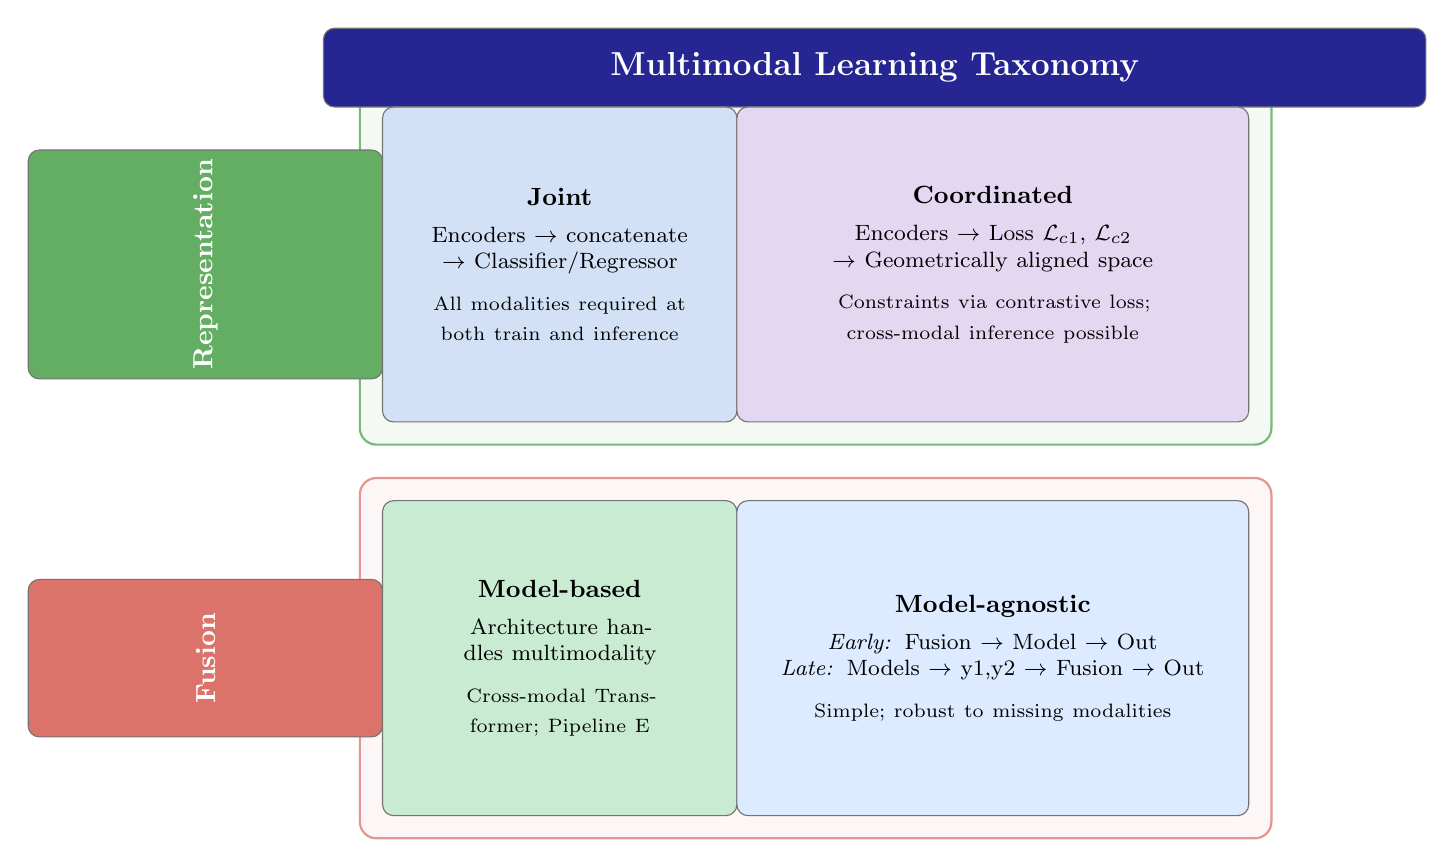
\begin{tikzpicture}[node distance=0.7cm and 1.1cm]
  \node[basebox,fill=NavyBlue!85,text=white,minimum width=14cm,minimum height=1cm,font=\large\bfseries] (hdr)
      at (0,0) {Multimodal Learning Taxonomy};

  \node[basebox,fill=ForestGreen!70,text=white,minimum width=2.0cm,minimum height=4.5cm,
        font=\bfseries,rotate=90,anchor=center] (repLabel) at (-8.5,-2.5) {Representation};
  \node[basebox,fill=coralred!80,text=white,minimum width=2.0cm,minimum height=4.5cm,
        font=\bfseries,rotate=90,anchor=center] (fusLabel) at (-8.5,-7.5) {Fusion};

  \node[basebox,fill=boxblue,minimum width=4.5cm,minimum height=4.0cm,
        text width=4.2cm] (joint) at (-4,-2.5)
      {\textbf{Joint}\\[4pt]
       \footnotesize Encoders $\to$ concatenate\\
       $\to$ Classifier/Regressor\\[4pt]
       \scriptsize All modalities required at both train and inference};

  \node[basebox,fill=boxpurple,minimum width=6.5cm,minimum height=4.0cm,
        text width=6.2cm] (coord) at (1.5,-2.5)
      {\textbf{Coordinated}\\[4pt]
       \footnotesize Encoders $\to$ Loss $\mathcal{L}_{c1}$, $\mathcal{L}_{c2}$\\
       $\to$ Geometrically aligned space\\[4pt]
       \scriptsize Constraints via contrastive loss; cross-modal inference possible};

  \node[basebox,fill=boxgreen,minimum width=4.5cm,minimum height=4.0cm,
        text width=4.2cm] (modelbased) at (-4,-7.5)
      {\textbf{Model-based}\\[4pt]
       \footnotesize Architecture handles multimodality\\[4pt]
       \scriptsize Cross-modal Transformer; Pipeline E};

  \node[basebox,fill=lightblue,minimum width=6.5cm,minimum height=4.0cm,
        text width=6.2cm] (modelagnostic) at (1.5,-7.5)
      {\textbf{Model-agnostic}\\[4pt]
       \footnotesize \textit{Early:} Fusion $\to$ Model $\to$ Out\\
       \textit{Late:} Models $\to$ y1,y2 $\to$ Fusion $\to$ Out\\[4pt]
       \scriptsize Simple; robust to missing modalities};

  \begin{pgfonlayer}{background}
    \node[rectangle,draw=ForestGreen!60,fill=ForestGreen!5,rounded corners=6pt,thick,
          fit=(joint)(coord),inner sep=8pt] {};
    \node[rectangle,draw=coralred!60,fill=coralred!5,rounded corners=6pt,thick,
          fit=(modelbased)(modelagnostic),inner sep=8pt] {};
  \end{pgfonlayer}
\end{tikzpicture}
}
\caption{Complete multimodal learning taxonomy. Top row (green): representation strategies. Bottom row (red): fusion strategies. MIVA-KNIGHT employs all four cells across its five pipelines.}
\label{fig:taxonomy_overview}
\end{figure}

\subsection{Joint Multi-Modal Representations}

Joint representations concatenate modality-specific encodings before a downstream task head.

\begin{definition}[Joint Representation]
Given modalities $\mathcal{M} = \{M_1, M_2, \ldots, M_K\}$ with encoder functions $f_k : \mathcal{X}_k \to \R^{d_k}$, the joint representation is:
\[
  \mathbf{r}_{\text{joint}} = \phi\!\left(\mathbf{e}_1, \mathbf{e}_2, \ldots, \mathbf{e}_K\right), \qquad \mathbf{e}_k = f_k(x_k)
\]
where $\phi$ is a pooling function (concatenation, element-wise sum, average, etc.).
\end{definition}

\begin{axiom}[Joint Representation Completeness]
A joint representation is \emph{complete} if $\phi$ is injective with respect to the modality tuple $(\mathbf{e}_1,\ldots,\mathbf{e}_K)$, i.e., distinct modality combinations produce distinct joint representations.
\end{axiom}

\begin{theorem}[Expressiveness of Concatenation]
Concatenation $\phi_{\text{cat}}(\mathbf{e}_1,\ldots,\mathbf{e}_K) = [\mathbf{e}_1;\ldots;\mathbf{e}_K] \in \R^{\sum_k d_k}$ is the maximal-rank pooling: a linear head $g_\theta$ with $g_\theta(\mathbf{r}) = W\mathbf{r} + b$ can learn arbitrary linear combinations of all modality features, while element-wise sum $\phi_{\text{sum}}$ constrains all $d_k$ to be equal and loses cross-modality interaction terms.
\end{theorem}

\begin{algorithm}[H]
\caption{Joint Multimodal Representation (Concatenation)}
\label{alg:joint_repr}
\begin{algorithmic}[1]
\Require Modality inputs $\{x_1, x_2, \ldots, x_K\}$; trained encoders $\{f_1,\ldots,f_K\}$; pooling function $\phi$; downstream head $g_\theta$
\Ensure Prediction $\hat{y}$, joint representation $\mathbf{r}$
\State \textbf{// Step 1: Encode each modality independently}
\For{$k = 1$ to $K$}
  \State $\mathbf{e}_k \gets f_k(x_k)$ \Comment{No gradient if encoder frozen}
\EndFor
\State \textbf{// Step 2: Pool representations}
\State $\mathbf{r}_{\text{joint}} \gets \phi(\mathbf{e}_1, \mathbf{e}_2, \ldots, \mathbf{e}_K)$
  \Comment{e.g., concat: $\mathbf{r} \in \R^{\sum_k d_k}$}
\State \textbf{// Step 3: Downstream task}
\State $\hat{y} \gets g_\theta(\mathbf{r}_{\text{joint}})$
\State \textbf{// Step 4 (training only): Compute loss and update $\theta$}
\If{training}
  \State $\mathcal{L} \gets \ell(\hat{y}, y)$ \Comment{Task-specific loss}
  \State $\theta \gets \theta - \eta\,\nabla_\theta \mathcal{L}$
\EndIf
\State \Return $(\hat{y},\; \mathbf{r}_{\text{joint}})$
\end{algorithmic}
\end{algorithm}

\subsection{Coordinated Multimodal Representations}

Coordinated representations learn modality-specific encodings that are \emph{aligned through a loss function}, without explicit concatenation.

\begin{definition}[Coordinated Representation via Contrastive Loss]
For modalities $M_1, M_2$ with encoders $f_1, f_2$ and positive pairs $\mathcal{P} = \{(x_1^{(i)}, x_2^{(i)})\}_{i=1}^N$:
\[
  \mathcal{L}_{\text{coord}} = \frac{1}{2}(\mathcal{L}_{c1} + \mathcal{L}_{c2})
\]
\[
  \mathcal{L}_{c1} = -\frac{1}{B}\sum_{i=1}^B \log\frac{\exp(\mathbf{e}_1^{(i)} \cdot \mathbf{e}_2^{(i)} / \tau)}{\sum_{j=1}^B \exp(\mathbf{e}_1^{(i)} \cdot \mathbf{e}_2^{(j)} / \tau)}, \quad
  \mathcal{L}_{c2} = -\frac{1}{B}\sum_{j=1}^B \log\frac{\exp(\mathbf{e}_2^{(j)} \cdot \mathbf{e}_1^{(j)} / \tau)}{\sum_{i=1}^B \exp(\mathbf{e}_2^{(j)} \cdot \mathbf{e}_1^{(i)} / \tau)}
\]
\end{definition}

\begin{lemma}[Coordinated vs.\ Joint Representations]
Coordinated representations require both modalities only during training (for the loss signal), not necessarily at inference. If $f_1$ encodes text and $f_2$ encodes images, a query may be issued via text alone and matched against pre-encoded image embeddings in the shared space. Joint representations require all modalities at inference.
\end{lemma}

\begin{algorithm}[H]
\caption{Coordinated Representation Learning (Symmetric Contrastive)}
\label{alg:coord_repr}
\begin{algorithmic}[1]
\Require Paired dataset $\mathcal{D} = \{(x_1^{(i)}, x_2^{(i)})\}_{i=1}^N$; encoders $f_1, f_2$; temperature $\tau = 0.07$
\Ensure Coordinated encoders mapping both modalities to shared $\Sph^{511}$
\For{each mini-batch $\mathcal{B} = \{(x_1^{(i)}, x_2^{(i)})\}_{i=1}^B$}
  \State $\mathbf{e}_1^{(i)} \gets f_1(x_1^{(i)})$; $\hat{\mathbf{e}}_1^{(i)} \gets \mathbf{e}_1^{(i)}/\Norm{\mathbf{e}_1^{(i)}}$ for $i=1\ldots B$
  \State $\mathbf{e}_2^{(i)} \gets f_2(x_2^{(i)})$; $\hat{\mathbf{e}}_2^{(i)} \gets \mathbf{e}_2^{(i)}/\Norm{\mathbf{e}_2^{(i)}}$ for $i=1\ldots B$
  \State $S_{ij} \gets \hat{\mathbf{e}}_1^{(i)} \cdot \hat{\mathbf{e}}_2^{(j)} / \tau$ \Comment{Similarity matrix $[B \times B]$}
  \State $\mathcal{L}_{c1} \gets -\frac{1}{B}\sum_{i=1}^B\log\frac{\exp(S_{ii})}{\sum_{j=1}^B \exp(S_{ij})}$
  \State $\mathcal{L}_{c2} \gets -\frac{1}{B}\sum_{j=1}^B\log\frac{\exp(S_{jj})}{\sum_{i=1}^B \exp(S_{ij})}$
  \State $\mathcal{L}_{\text{coord}} \gets \frac{1}{2}(\mathcal{L}_{c1} + \mathcal{L}_{c2})$
  \State $\mathcal{L}_{\text{coord}}.\text{backward()}$; step optimiser
\EndFor
\end{algorithmic}
\end{algorithm}

\subsection{Handling Missing Modalities}

\begin{definition}[Missing Modality Problem]
A sample $\mathbf{x} = (x_1, x_2, \ldots, x_K)$ has a \emph{missing modality} $M_k$ if $x_k$ is unavailable at inference time. The system must produce a valid prediction using only the available subset $\mathcal{A} \subseteq \{1,\ldots,K\}$.
\end{definition}

\begin{axiom}[Zero-Vector Missing Modality]
\label{ax:missing}
If modality $M_k$ is absent, substituting $\mathbf{e}_k = \bm{0} \in \R^{d_k}$ in a linear projection layer results in zero contribution: $W_k \bm{0} = \bm{0}$. This provides graceful degradation without injecting noise.
\end{axiom}

\begin{algorithm}[H]
\caption{Missing-Modality Robust Inference}
\label{alg:missing_modal}
\begin{algorithmic}[1]
\Require Available modalities $\mathcal{A} \subseteq \{1,\ldots,K\}$; missing modalities $\mathcal{M} = \{1,\ldots,K\}\setminus\mathcal{A}$
\Require Projection weights $\{W_k\}$; fusion function $\phi$
\Ensure Robust representation $\mathbf{r}$
\For{$k = 1$ to $K$}
  \If{$k \in \mathcal{A}$}
    \State $\mathbf{e}_k \gets f_k(x_k)$; $\hat{\mathbf{e}}_k \gets \mathbf{e}_k / \Norm{\mathbf{e}_k}$
  \Else
    \State $\hat{\mathbf{e}}_k \gets \bm{0}^d$ \Comment{Zero-token for missing modality (Axiom~\ref{ax:missing})}
  \EndIf
\EndFor
\State $\mathbf{r} \gets \phi(\hat{\mathbf{e}}_1, \ldots, \hat{\mathbf{e}}_K)$
\If{all $k \notin \mathcal{A}$}
  \State \Return \textsc{UncertaintyResponse}()
\EndIf
\State \Return $\mathbf{r}$
\end{algorithmic}
\end{algorithm}

\subsection{Model-Based Multimodal Fusion (Cross-Modal Transformer)}

\begin{definition}[Model-Based Fusion]
In model-based fusion, the joint prediction arises from a single model $\pi_\Theta : \mathcal{X}_1 \times \cdots \times \mathcal{X}_K \to \mathcal{Y}$:
\[
  \hat{y} = \pi_\Theta(x_1, x_2, \ldots, x_K)
\]
The model architecture itself (e.g., cross-modal attention) is what enables multimodal reasoning.
\end{definition}

\begin{theorem}[Cross-Modal Attention Expressiveness]
Multi-head attention with $h$ heads over $K$ modality tokens learns $h$ independent linear combinations of modality interactions. For $K=3$ modalities and $h=8$ heads, each head can specialise in a distinct pairwise relationship (text-audio, audio-video, text-video) plus higher-order combinations, without manual feature engineering.
\end{theorem}

\begin{algorithm}[H]
\caption{Model-Based Multimodal Fusion (Cross-Modal Transformer)}
\label{alg:model_based_fusion}
\begin{algorithmic}[1]
\Require Modality embeddings $\{\hat{\mathbf{e}}_k\}_{k=1}^K$, each $\in \R^d$; Transformer parameters $\Theta$
\Ensure Fused representation $\mathbf{r}_{\text{fused}} \in \R^d$
\State $X \gets \text{stack}([\hat{\mathbf{e}}_1, \hat{\mathbf{e}}_2, \ldots, \hat{\mathbf{e}}_K],\; \text{dim}=1)$ \Comment{$[B, K, d]$}
\State $X \gets X + P$ \Comment{$P \in \R^{K \times d}$ learned modality tags}
\For{layer $\ell = 1$ to $L$}
  \State $X \gets X + \MHA(\LN(X))$ \Comment{Pre-LN cross-modal attention}
  \State $X \gets X + \text{FFN}(\LN(X))$ \Comment{Pre-LN feed-forward}
\EndFor
\State $\mathbf{r}_{\text{fused}} \gets \frac{1}{K}\sum_{k=1}^K X_{:,k,:}$ \Comment{Mean-pool over modality tokens}
\State $\hat{y} \gets g_\theta(\mathbf{r}_{\text{fused}})$
\State \Return $(\hat{y}, \mathbf{r}_{\text{fused}})$
\end{algorithmic}
\end{algorithm}

\subsection{Model-Agnostic Early and Late Fusion}

\begin{definition}[Early Fusion]
Features from all modalities are combined into a single representation $\mathbf{z} = \phi_{\text{early}}(x_1, \ldots, x_K)$ before any learned model is applied:
$\hat{y} = g_\theta(\phi_{\text{early}}(x_1, \ldots, x_K))$.
\end{definition}

\begin{definition}[Late Fusion]
$K$ independent models $\{g_k\}_{k=1}^K$ each produce $\hat{y}_k = g_k(x_k)$. A fusion function combines these:
$\hat{y} = \phi_{\text{late}}(\hat{y}_1, \ldots, \hat{y}_K)$.
Common choices: mean, weighted mean, learned MLP combiner.
\end{definition}

\begin{lemma}[Early Fusion Trade-off]
Early fusion achieves the lowest inference latency (single forward pass) but requires all modalities to be present and aligned. Missing modalities cannot be trivially handled without imputation.
\end{lemma}

\begin{proposition}[Late Fusion Missing-Modality Robustness]
Late fusion is the most robust to missing modalities: if $M_k$ is absent, the weight $w_k$ can be set to zero and the remaining modalities re-normalised: $\hat{y} = \frac{\sum_{k \in \mathcal{A}} w_k \hat{y}_k}{\sum_{k \in \mathcal{A}} w_k}$, requiring no architectural changes.
\end{proposition}

%%
%% ============================================================
%% PART IV — THE FIVE MML CHALLENGES
%% ============================================================
%%
\newpage
\section{The Five Multimodal Machine Learning Challenges}
\label{sec:fivechallenges}

\begin{tcolorbox}[keybox,title={Five Canonical MML Challenges in MIVA-KNIGHT}]
\begin{tabular}{lll}
\toprule
\textbf{Challenge} & \textbf{Core Problem} & \textbf{MIVA-KNIGHT Realisation} \\
\midrule
1.~Representation & Encode $\MA, \MB \to$ shared space & $\Sph^{511}$, InfoNCE, Pipelines A--D \\
2.~Translation & $\MA \to \MB$ mapping & Whisper STT, gTTS TTS, LLM captioning \\
3.~Fusion & Combine modalities $\to$ prediction & Cross-modal Transformer, Pipeline E \\
4.~Co-learning & Transfer knowledge between modalities & ROCO surgical transfer (2.23\%) \\
5.~Alignment & Segment $\MA$ $\leftrightarrow$ segment $\MB$ & CMU-MOSI temporal attention alignment \\
\bottomrule
\end{tabular}
\end{tcolorbox}

\subsection{Challenge 1: Multimodal Representation}

\begin{tcolorbox}[challengebox,title={Challenge 1: Representation}]
\textbf{Core question}: How do we represent modalities $\MA$ and $\MB$ so that semantically related content from each modality maps to nearby points in a shared vector space?
\end{tcolorbox}

\begin{definition}[Multimodal Representation Problem]
Given modalities $\MA$ and $\MB$ with raw data spaces $\mathcal{X}_A$ and $\mathcal{X}_B$, the representation problem is to learn encoder functions $f_A : \mathcal{X}_A \to \R^d$ and $f_B : \mathcal{X}_B \to \R^d$ such that for matching pairs:
\[
  \text{sim}(f_A(x_A^{(i)}), f_B(x_B^{(i)})) \gg \text{sim}(f_A(x_A^{(i)}), f_B(x_B^{(j)})) \quad \forall\; j \ne i.
\]
\end{definition}

\begin{definition}[Symmetric InfoNCE Loss]
For batch size $B$, temperature $\tau = 0.07$, similarity $S_{ij} = \hat{e}_A^{(i)} \cdot \hat{e}_B^{(j)} / \tau$:
\[
  \mathcal{L}_{\text{InfoNCE}} = \frac{1}{2}\left[
    -\frac{1}{B}\sum_i \log\frac{e^{S_{ii}}}{\sum_j e^{S_{ij}}}
    -\frac{1}{B}\sum_j \log\frac{e^{S_{jj}}}{\sum_i e^{S_{ij}}}
  \right]
\]
\end{definition}

\begin{theorem}[InfoNCE as Mutual Information Bound]
\[
  I(f_A(x_A);\, f_B(x_B)) \ge \log B - \mathcal{L}_{\text{InfoNCE}}
\]
Minimising $\mathcal{L}_{\text{InfoNCE}}$ maximises a lower bound on the mutual information between the two modality representations.
\end{theorem}

\begin{lemma}[Random Baseline Loss]
At random initialisation, $\EE[\mathcal{L}_{\text{InfoNCE}}] = \log B$. For $B = 32$: $\log 32 \approx 3.47$.
\end{lemma}

\begin{theorem}[Representation Quality Upper Bound]
For any encoder $f_A$ and paired dataset of size $N$, the achievable Precision@1 is upper-bounded by:
\[
  P@1 \le 1 - \frac{H(Y|\hat{e}_A)}{H(Y)}
\]
where $Y$ is the ground-truth match label and $H$ is entropy.
\end{theorem}

\begin{algorithm}[H]
\caption{Challenge 1 — Multimodal Representation Learning (Coordinated Embedding)}
\label{alg:repr_challenge}
\begin{algorithmic}[1]
\Require Paired dataset $\mathcal{D} = \{(x_A^{(i)}, x_B^{(i)})\}_{i=1}^N$
\Require Frozen encoders $f_A, f_B$; trainable projection heads $P_A, P_B$ (Def.~\ref{def:projmlp})
\Require Temperature $\tau = 0.07$; batch size $B$; AdamW with lr\,$= 10^{-4}$
\Ensure Trained $P_A^*, P_B^*$ embedding both modalities into shared $\Sph^{511}$
\For{epoch $= 1$ to $E$}
  \ForEach{mini-batch $\{(x_A^{(i)}, x_B^{(i)})\}_{i=1}^B$}
    \State $h_A^{(i)} \gets f_A(x_A^{(i)})$ for $i=1\ldots B$ \Comment{Frozen backbone, no grad}
    \State $h_B^{(i)} \gets f_B(x_B^{(i)})$ for $i=1\ldots B$
    \State $\hat{e}_A^{(i)} \gets P_A(h_A^{(i)}) / \Norm{P_A(h_A^{(i)})}_2 \in \Sph^{511}$
    \State $\hat{e}_B^{(i)} \gets P_B(h_B^{(i)}) / \Norm{P_B(h_B^{(i)})}_2 \in \Sph^{511}$
    \State $S_{ij} \gets \hat{e}_A^{(i)} \cdot \hat{e}_B^{(j)} / \tau \quad \forall\, i,j$ \Comment{$[B \times B]$ matrix}
    \State $\mathcal{L}_{A \to B} \gets -\frac{1}{B}\sum_i \log\frac{e^{S_{ii}}}{\sum_j e^{S_{ij}}}$
    \State $\mathcal{L}_{B \to A} \gets -\frac{1}{B}\sum_j \log\frac{e^{S_{jj}}}{\sum_i e^{S_{ij}}}$
    \State $\mathcal{L}_{\text{repr}} \gets \frac{1}{2}(\mathcal{L}_{A \to B} + \mathcal{L}_{B \to A})$
    \State optimizer.zero\_grad(); $\mathcal{L}_{\text{repr}}$.backward(); clip\_grad$(1.0)$; optimizer.step()
  \EndFor
  \State Evaluate: P@1, P@3, MRR on validation set
\EndFor
\State \Return $(P_A^*, P_B^*)$
\end{algorithmic}
\end{algorithm}

\subsection{Challenge 2: Multimodal Translation}

\begin{tcolorbox}[challengebox,title={Challenge 2: Translation}]
\textbf{Core question}: Given an observation in Modality~A, how do we generate a meaningful, accurate representation in Modality~B?
\end{tcolorbox}

\begin{definition}[Multimodal Translation]
The translation task is to generate $\hat{x}_B \in \mathcal{X}_B$ from $x_A \in \mathcal{X}_A$ such that $\hat{x}_B$ is \emph{faithful} (accurately reflects $x_A$) and \emph{fluent} (natural in $\mathcal{X}_B$).
\end{definition}

\begin{theorem}[Faithfulness vs.\ Fluency Trade-off]
For any translation model $g : \mathcal{X}_A \to \mathcal{X}_B$, expected faithfulness $F$ and fluency $Q$ satisfy:
$F \cdot Q \le \frac{1}{4}(F + Q)^2$.
Maximising one without constraint on the other produces a degenerate translator.
\end{theorem}

\begin{axiom}[Grounding Constraint]
\label{ax:grounding}
A faithful translation must be grounded: every claim in $\hat{x}_B$ must be inferable from $x_A$ or a verified knowledge source. MIVA-KNIGHT enforces this via RAG: the LLM translates retrieved context, not its parametric knowledge.
\end{axiom}

\begin{definition}[Whisper CTC-Attention Architecture]
Whisper is a seq2seq model: $P(\hat{q} \mid x_s) = \prod_{t=1}^T P(q_t \mid q_{1:t-1},\, \text{Enc}(x_s))$ where Enc is a convolutional + Transformer encoder over mel-spectrogram frames, and Dec is an autoregressive Transformer decoder.
\end{definition}

\begin{algorithm}[H]
\caption{Challenge 2 --- Multimodal Translation (Three Pathways)}
\label{alg:trans_challenge}
\begin{algorithmic}[1]
\Require Input $x$ of source modality $\MA$; target modality $\MB \in \{\text{text, image, audio}\}$
\Ensure Translation $\hat{x}_B$ in target modality $\MB$
\Procedure{Translate}{$x, \MA, \MB$}
\If{$\MA = \text{speech}$, $\MB = \text{text}$} \Comment{\textbf{Pathway 1: Speech-to-Text (STT)}}
  \State Resample $x$ to 16\,kHz mono; compute log-mel spectrogram (80 bins)
  \State $\hat{q} \gets \text{Whisper.decode}(\text{mel}, \text{language}=\text{``en''})$
  \State \Return $\hat{q}$
\EndIf
\If{$\MA = \text{image}$, $\MB = \text{caption/text}$} \Comment{\textbf{Pathway 2: Image-to-Caption}}
  \State $h_I \gets \text{ResNet50}(x)$ \Comment{pool5 features $[2048]$}
  \State $\hat{e}_I \gets P_I(h_I) / \Norm{P_I(h_I)}_2 \in \Sph^{511}$
  \State $\mathcal{D}^* \gets \text{HybridRetriever.retrieve}(\hat{e}_I)$
  \State $\Pi \gets$ ``Describe the image using ONLY these captions: $\mathcal{D}^*$''
  \State $\hat{x}_B \gets \text{LLM.generate}(\Pi)$
  \State \Return $\hat{x}_B$
\EndIf
\If{$\MA = \text{text}$, $\MB = \text{audio}$} \Comment{\textbf{Pathway 3: Text-to-Speech (TTS)}}
  \State buf $\gets$ BytesIO(); $\text{gTTS}(x).\text{write\_to\_fp}(\text{buf})$; buf.seek(0)
  \State \Return buf.read() \Comment{MP3 bytes, no disk I/O}
\EndIf
\EndProcedure
\end{algorithmic}
\end{algorithm}

\subsection{Challenge 3: Multimodal Fusion}

\begin{tcolorbox}[challengebox,title={Challenge 3: Fusion}]
\textbf{Core question}: How do we combine signals from multiple modalities to make a single prediction that outperforms any single-modality model?
\end{tcolorbox}

\begin{definition}[Multimodal Fusion Problem]
Given embeddings $\eA \in \R^{d_A}$ and $\eB \in \R^{d_B}$, learn $g : \R^{d_A} \times \R^{d_B} \to \mathcal{Y}$ outperforming any unimodal predictor.
\end{definition}

\begin{axiom}[Fusion Benefit]
\label{ax:fusion}
Fusion is beneficial iff the modalities are \emph{complementary}: $I((\eA, \eB); Y) > \max(I(\eA; Y), I(\eB; Y))$.
\end{axiom}

\begin{definition}[Multi-Task Fusion Loss --- Pipeline E]
\[
  \mathcal{L}_{\text{fusion}}(\hat{y}, y, b) = 0.6 \cdot \mathcal{L}_{\text{MSE}}(\hat{y}, y) + 0.4 \cdot \mathcal{L}_{\text{BCE}}(\hat{y}, b)
\]
where $y \in [-3,+3]$ (regression), $b \in \{0,1\}$ (binary).
\end{definition}

\begin{theorem}[Stable BCE with Logits]
\[
  \mathcal{L}_{\text{BCE}}(\hat{y}, b) = \max(0, \hat{y}) - b\hat{y} + \log(1 + e^{-|\hat{y}|})
\]
This numerically stable form avoids overflow in $e^{\hat{y}}$ for large positive $\hat{y}$.
\end{theorem}

\begin{algorithm}[H]
\caption{Challenge 3 --- Multimodal Fusion (Cross-Modal Transformer, Pipeline E)}
\label{alg:fusion_challenge}
\begin{algorithmic}[1]
\Require Modality embeddings $\hat{e}_1, \hat{e}_2, \ldots, \hat{e}_K \in \R^{512}$; parameters $\theta$
\Require Ground-truth $y$ (continuous), $b$ (binary)
\Ensure Prediction $\hat{y}$; loss $\mathcal{L}_{\text{fusion}}$
\State $X \gets \text{stack}([\hat{e}_1,\ldots,\hat{e}_K], \text{dim}=1) \in \R^{B \times K \times 512}$
\State $X \gets X + P$ \Comment{Learnable modality positional encodings}
\For{$\ell = 1$ to $L=2$}
  \State $X \gets X + \MHA(\LN(X))$ \Comment{Pre-LN self-attention across all modalities}
  \State $X \gets X + \text{FFN}(\LN(X))$
\EndFor
\State $\bar{x} \gets X.\text{mean(dim=1)} \in \R^{B \times 512}$
\State $\hat{y} \gets W_2(\GELU(W_1 \bar{x})) \in \R^B$ \Comment{$512 \to 256 \to 1$}
\State $\mathcal{L}_{\text{MSE}} \gets \frac{1}{B}\sum({\hat{y} - y})^2$
\State $\mathcal{L}_{\text{BCE}} \gets \text{binary\_cross\_entropy\_with\_logits}(\hat{y}, b)$
\State $\mathcal{L}_{\text{fusion}} \gets 0.6 \cdot \mathcal{L}_{\text{MSE}} + 0.4 \cdot \mathcal{L}_{\text{BCE}}$
\State optimizer.zero\_grad(); $\mathcal{L}_{\text{fusion}}$.backward(); optimizer.step()
\State \Return $(\hat{y}, \mathcal{L}_{\text{fusion}})$
\end{algorithmic}
\end{algorithm}

\subsection{Challenge 4: Co-learning}

\begin{tcolorbox}[challengebox,title={Challenge 4: Co-learning}]
\textbf{Core question}: How can a strong modality help train a weaker modality, especially when the weaker modality has limited labelled data?
\end{tcolorbox}

\begin{definition}[Surgical Co-learning Transfer]
\label{def:surgical}
Given source domain $\mathcal{D}_{\text{src}}$ (COCO, trained) and target domain $\mathcal{D}_{\text{tgt}}$ (ROCO, new), surgical transfer trains only the domain-specific projection head $P_I^{\text{tgt}}$:
\[
  \phi^* = \argmin_\phi \mathcal{L}_{\text{co}}(\phi) = \mathcal{L}_{\text{InfoNCE}}(P_I^\phi \circ f_I, f_T) + \lambda \mathcal{L}_{\text{distill}}(\phi)
\]
\[
  \mathcal{L}_{\text{distill}}(\phi) = \frac{1}{B}\sum_{i=1}^B \Norm{f_T^{\text{tgt}}(c_i) - f_T^{\text{src}}(c_i)}_2^2
\]
\end{definition}

\begin{theorem}[Surgical Transfer Efficiency]
Under Definition~\ref{def:surgical}, only $5.25\,\text{M}$ out of $235.15\,\text{M}$ total parameters are modified:
\[
  \eta_{\text{surgical}} = \frac{5.25}{235.15} \approx 2.23\%.
\]
\end{theorem}

\begin{axiom}[Minimal Retraining Principle]
Only the module responsible for translating domain-specific features into the shared embedding space (ImageProjection) is retrained per domain. All upstream encoders serve as immutable feature extractors.
\end{axiom}

\begin{lemma}[Domain Swap Isolation]
Replacing $P_I^{\text{src}} \to P_I^{\text{tgt}}$ does not move existing text or audio embeddings in $\Sph^{511}$. Medical domain transfer cannot degrade general-domain text retrieval.
\end{lemma}

\subsection{Challenge 5: Multimodal Alignment}

\begin{tcolorbox}[challengebox,title={Challenge 5: Alignment}]
\textbf{Core question}: How do we find corresponding sub-elements of $\MA$ and $\MB$ without explicit supervision of the correspondence?
\end{tcolorbox}

\begin{definition}[Multimodal Alignment Problem]
Given sequences $X_A = [x_A^{(1)},\ldots,x_A^{(T_A)}]$ and $X_B = [x_B^{(1)},\ldots,x_B^{(T_B)}]$, the alignment problem is to find a mapping $\alpha : \{1,\ldots,T_A\} \to \{1,\ldots,T_B\}$ such that $x_A^{(t)}$ and $x_B^{(\alpha(t))}$ correspond semantically.
\end{definition}

\begin{theorem}[Attention as Soft Alignment]
In the cross-modal Transformer of Pipeline E, the attention matrix $\text{Attn}(Q, K, V)_{ti'} = \frac{\exp(Q_t \cdot K_{t'}/\sqrt{d_k})}{\sum_{t''}\exp(Q_t \cdot K_{t''}/\sqrt{d_k})}$ provides a soft differentiable alignment between audio waveform segments (rows) and text tokens (columns) in the CMU-MOSI dataset.
\end{theorem}

\begin{algorithm}[H]
\caption{Challenge 5 --- Temporal Alignment via Cross-Modal Attention (CMU-MOSI)}
\label{alg:alignment_challenge}
\begin{algorithmic}[1]
\Require Audio segments $\{e_A^{(t)}\}_{t=1}^{T_A}$; text tokens $\{e_T^{(t')}\}_{t'=1}^{T_B}$; attention heads $h$
\Ensure Soft alignment matrix $\text{Align} \in \R^{T_A \times T_B}$; sentiment $\hat{y}$
\State Stack tokens: $X \gets [e_T^{(1)},\ldots,e_T^{(T_B)}, e_A^{(1)},\ldots,e_A^{(T_A)}] \in \R^{(T_A+T_B) \times 512}$
\State $Q \gets XW^Q$; $K \gets XW^K$; $V \gets XW^V$ \Comment{Project to head dimension $d_k = 64$}
\State $\text{Attn} \gets \softmax(QK^\top / \sqrt{d_k}) \in \R^{(T_A+T_B) \times (T_A+T_B)}$
\State $\text{Align} \gets \text{Attn}[T_B{:},\; :T_B]$ \Comment{Audio-to-text sub-block}
\State \Comment{Each row: how much attention audio segment $t$ pays to each text token $t'$}
\State $Z \gets \text{Attn} \cdot V$; mean-pool; regression head $\to \hat{y}$
\State \Return $(\text{Align}, \hat{y})$
\end{algorithmic}
\end{algorithm}

%%
%% ============================================================
%% PART V — PIPELINE A: GENERAL DOMAIN (COCO)
%% ============================================================
%%
\newpage
\section{Pipeline A: General Domain --- COCO Text-Image Retrieval}
\label{sec:pipelineA}

\subsection{Overview}

Pipeline~A trains a coordinated multimodal embedding on the COCO val2017 dataset (202,654 image-caption pairs) using symmetric InfoNCE loss, building the foundation for the shared $\Sph^{511}$ space.

\begin{figure}[H]
\centering
\resizebox{\textwidth}{!}{%
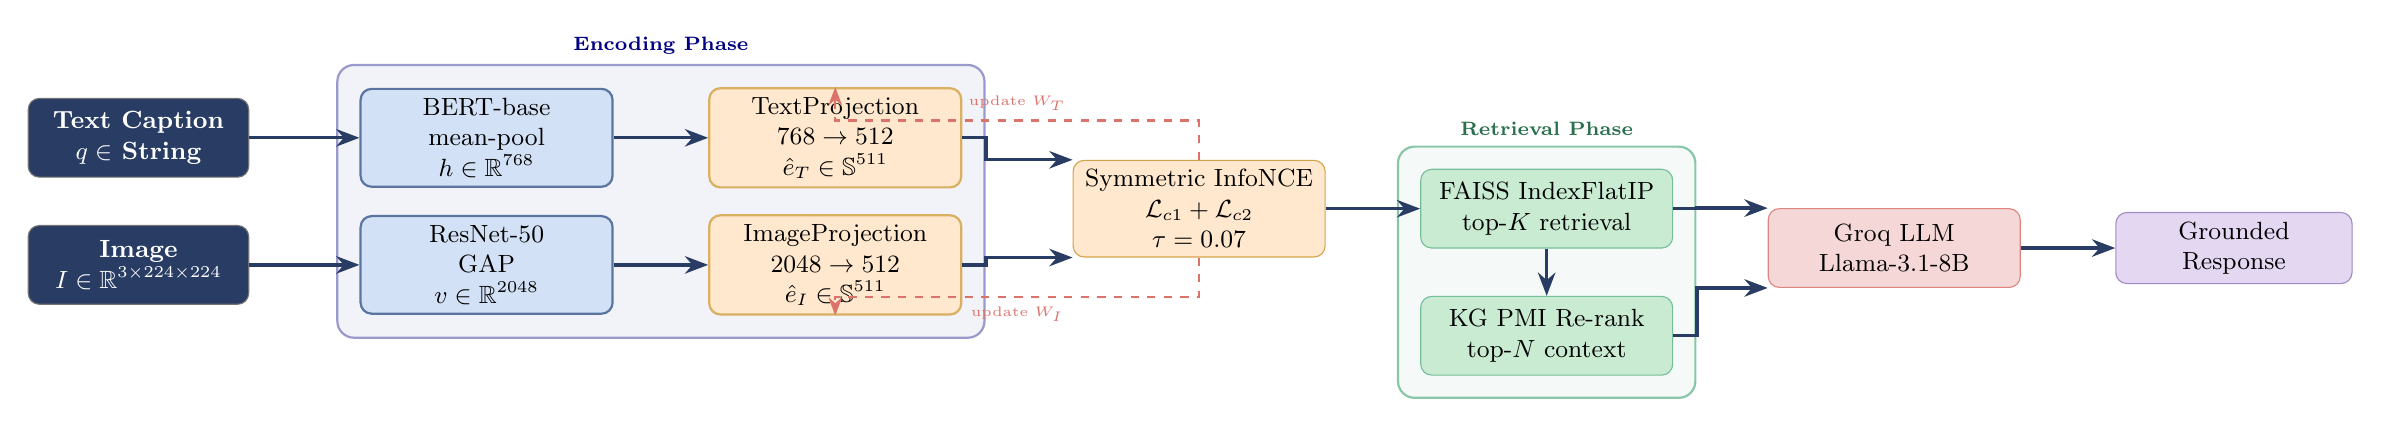
\begin{tikzpicture}[node distance=0.7cm and 1.0cm]
  \node[inputnode] (textq) at (0,0) {Text Caption\\$q \in$ String};
  \node[inputnode,below=0.6cm of textq] (imgq) {Image\\$I \in \R^{3\times224\times224}$};

  \node[encnode,right=1.4cm of textq] (bert) {BERT-base\\mean-pool\\$h \in \R^{768}$};
  \node[encnode,right=1.4cm of imgq] (resnet) {ResNet-50\\GAP\\$v \in \R^{2048}$};

  \node[projnode,right=1.2cm of bert] (tproj) {TextProjection\\$768 \to 512$\\$\hat{e}_T \in \Sph^{511}$};
  \node[projnode,right=1.2cm of resnet] (iproj) {ImageProjection\\$2048 \to 512$\\$\hat{e}_I \in \Sph^{511}$};

  \node[lossnode,right=1.4cm of tproj,yshift=-0.9cm] (loss) {Symmetric InfoNCE\\$\mathcal{L}_{c1} + \mathcal{L}_{c2}$\\$\tau = 0.07$};

  \node[retnode,right=1.2cm of loss] (faiss) {FAISS IndexFlatIP\\top-$K$ retrieval};
  \node[retnode,below=0.6cm of faiss] (kg) {KG PMI Re-rank\\top-$N$ context};
  \node[gennode,right=1.2cm of faiss,yshift=-0.5cm] (llm) {Groq LLM\\Llama-3.1-8B};
  \node[outnode,right=1.2cm of llm] (out) {Grounded\\Response};

  \draw[thickarr] (textq)--(bert); \draw[thickarr] (imgq)--(resnet);
  \draw[thickarr] (bert)--(tproj); \draw[thickarr] (resnet)--(iproj);
  \draw[thickarr] (tproj.east) -- ++(0.3,0) |- (loss.north west);
  \draw[thickarr] (iproj.east) -- ++(0.3,0) |- (loss.south west);
  \draw[redarr,dashed] (loss.north) -- ++(0,0.5) -| (tproj.north)
      node[near start,above,font=\tiny]{update $W_T$};
  \draw[redarr,dashed] (loss.south) -- ++(0,-0.5) -| (iproj.south)
      node[near start,below,font=\tiny]{update $W_I$};
  \draw[thickarr] (loss.east) -- ++(0.3,0) |- (faiss.west);
  \draw[thickarr] (faiss.south)--(kg.north);
  \draw[thickarr] (faiss.east) -- ++(0.3,0) |- (llm.north west);
  \draw[thickarr] (kg.east) -- ++(0.3,0) |- (llm.south west);
  \draw[thickarr] (llm)--(out);

  \begin{pgfonlayer}{background}
    \node[rectangle,draw=NavyBlue!40,fill=NavyBlue!5,rounded corners=6pt,thick,
          fit=(bert)(resnet)(tproj)(iproj),inner sep=8pt,
          label={[font=\scriptsize\bfseries,color=NavyBlue]above:Encoding Phase}] {};
    \node[rectangle,draw=mintgreen!60,fill=mintgreen!5,rounded corners=6pt,thick,
          fit=(faiss)(kg),inner sep=8pt,
          label={[font=\scriptsize\bfseries,color=mintgreen!70!black]above:Retrieval Phase}] {};
  \end{pgfonlayer}
\end{tikzpicture}
}
\caption{Pipeline~A architecture: COCO text-image coordinated embedding with two-stage RAG retrieval.}
\label{fig:pipeline_a}
\end{figure}

\subsection{Text Encoder: BERT Mean-Pool + TextProjection}

\begin{definition}[TextProjection $f_T$]
$f_T : \R^{768} \to \Sph^{511}$ defined by Definition~\ref{def:projmlp} with $d_{\text{in}} = 768$. Trainable parameters: $\approx$1.6\,M.
\end{definition}

\begin{remark}[Mean Pooling vs.\ CLS]
CLS token ($H_{:,0,:}$) is optimised for classification but degrades for long sequences. Mean pooling ($\frac{1}{T}\sum H_{:,t,:}$) provides better semantic similarity for retrieval tasks (consistent with sentence-transformers literature).
\end{remark}

\begin{algorithm}[H]
\caption{TextEncoderV2.encode --- BERT Mean-Pool + TextProjection}
\label{alg:textencode}
\begin{algorithmic}[1]
\Require Text $t \in$ String; frozen BERT; trained TextProjection $P_\theta$ (Def.~\ref{def:projmlp}, $d_{\text{in}}=768$)
\Ensure $e_q \in \Sph^{511}$, entity set $\mathcal{E}_q$, domain hint
\State \textbf{Tokenise:} $\text{tokens} \gets \text{WordPiece}(t, \texttt{max\_length}=128, \texttt{truncation=True})$
\State \textbf{BERT forward} (no grad):
  $H \gets \text{BERT}(\text{tokens}).\text{last\_hidden\_state} \in \R^{1 \times T \times 768}$
\State \textbf{Mean pool:} $h_{\text{BERT}} \gets \frac{1}{T}\sum_{t=1}^T H_{:,t,:} \in \R^{768}$
\State \textbf{Project:} $e_{\text{raw}} \gets P_\theta(h_{\text{BERT}}) \in \R^{512}$
\State \textbf{Normalise:} $e_q \gets e_{\text{raw}} / \Norm{e_{\text{raw}}}_2$
\State \textbf{NER:} $\mathcal{E}_q \gets \{\text{noun chunks}\} \cup \{\text{named entities}\}$ (lowercased)
\State domain\_hint $\gets$ ``medical'' if $|\{w \in \textsc{Medical\_Terms} : w \subseteq t.\text{lower}()\}| \ge 2$ else None
\State \Return $(e_q,\; \mathcal{E}_q,\; \text{domain\_hint})$
\end{algorithmic}
\end{algorithm}

\subsection{Image Encoder: ResNet-50 + ImageProjection}

\begin{definition}[ImageProjection $f_\phi$]
\[
  f_\phi : \R^{2048} \to \Sph^{511}, \qquad
  f_\phi(x) = \frac{g_\phi(x)}{\Norm{g_\phi(x)}_2}
\]
\[
  g_\phi(x) = \LN_{512}\!\left(W_2 \cdot \GELU(\LN_{2048}(W_1 x + b_1)) + b_2\right)
\]
where $W_1 \in \R^{2048 \times 2048}$, $W_2 \in \R^{512 \times 2048}$. Total: $\approx$5.25\,M parameters.
\end{definition}

\begin{axiom}[Mandatory ImageNet Normalisation]
Input images must be normalised per channel:
\[
  \hat{x}_{c,h,w} = \frac{x_{c,h,w} - \mu_c}{\sigma_c}, \quad
  \bm{\mu} = [0.485, 0.456, 0.406], \quad \bm{\sigma} = [0.229, 0.224, 0.225].
\]
ResNet-50 BatchNorm layers are calibrated with these statistics; deviations degrade pool5 features.
\end{axiom}

\begin{algorithm}[H]
\caption{Pipeline A Training Epoch (Symmetric InfoNCE)}
\label{alg:trainepoch_A}
\begin{algorithmic}[1]
\Require COCO DataLoader $L$; TextProjection $P_\theta$; ImageProjection $f_\phi$; $\tau = 0.07$
\Ensure Updated $P_\theta, f_\phi$; epoch loss
\State total\_loss $\gets 0$
\ForEach{batch $(I^{B \times 3 \times 224 \times 224},\; T^B)$ in $L$}
  \State $\hat{e}_T^{(b)} \gets \textsc{TextEncoderV2}(T[b])$ for $b=1\ldots B$ \quad $\Rightarrow E_T \in \R^{B \times 512}$
  \State $\hat{e}_I^{(b)} \gets f_\phi(\text{ResNet50}(I[b]))$ for $b=1\ldots B$ \quad $\Rightarrow E_I \in \R^{B \times 512}$
  \State $S \gets E_T \cdot E_I^\top \in \R^{B \times B}$; \quad $\mathcal{L} \gets \mathcal{L}_{\text{InfoNCE}}(E_T, E_I, \tau)$
  \State optimizer.zero\_grad(); $\mathcal{L}$.backward()
  \State clip\_grad\_norm$(\nabla\theta, c=1.0)$; optimizer.step(); scheduler.step()
  \State total\_loss $\mathrel{+}= \mathcal{L}$.item()
\EndFor
\State \Return total\_loss / $|L|$
\end{algorithmic}
\end{algorithm}

%%
%% ============================================================
%% PART VI — KNOWLEDGE GRAPH CONSTRUCTION
%% ============================================================
%%
\newpage
\section{Knowledge Graph: PMI-Weighted Entity Graph}
\label{sec:kg}

\begin{definition}[General Knowledge Graph $\KG_G$]
\[
  \KG_G = (\mathcal{V}_G, \mathcal{E}_G, w), \quad
  \mathcal{V}_G = \text{top-2000 COCO entities (spaCy)}, \quad
  (a,b) \in \mathcal{E}_G \Leftrightarrow \text{PMI}(a,b) > 0.
\]
\[
  \text{PMI}(a,b) = \log\frac{c_{ab} \cdot N}{f_a \cdot f_b + \varepsilon}, \quad w(a,b) = \text{PMI}(a,b).
\]
\end{definition}

\begin{axiom}[PMI Semantic Association]
$\text{PMI}(a,b) > 0 \Leftrightarrow$ entities $a, b$ co-occur more than expected under independence.
\end{axiom}

\begin{algorithm}[H]
\caption{Build NER Knowledge Graph (PMI-Weighted)}
\label{alg:kg_build}
\begin{algorithmic}[1]
\Require $N$ captions; spaCy \texttt{en\_core\_web\_sm}; top-$V = 2000$ entities
\Ensure \texttt{ner\_kg.pkl}: $\text{dict}[\text{entity} \to \text{dict}[\text{entity} \to \text{PMI}]]$
\For{captions in batches of 1,000}
  \State $\mathcal{E}_{\text{doc}} \gets \{\text{noun chunks}\} \cup \{\text{named entities}\}$ (lowercased)
  \State Append to all\_doc\_entities
\EndFor
\State entity\_freq $\gets \text{Counter}(\bigcup \mathcal{E}_{\text{doc}})$
\State $\mathcal{V}_G \gets \text{top-}V$ entities with freq $\ge 5$
\For{each document entity set $E_i$ (filtered to $\mathcal{V}_G$)}
  \For{each symmetric pair $(a,b) \in E_i \times E_i,\; a \ne b$}
    \State cooc$[a][b] \mathrel{+}= 1$; cooc$[b][a] \mathrel{+}= 1$
  \EndFor
\EndFor
\For{each $a \in \mathcal{V}_G$ with freq $\ge 5$}
  \For{each $(b, c_{ab})$ with $c_{ab} \ge 3$}
    \State $\text{pmi} \gets \log(c_{ab} \cdot N / (f_a \cdot f_b + \varepsilon))$
    \If{pmi $> 0$} $\KG_G[a][b] \gets \text{pmi}$ \EndIf
  \EndFor
\EndFor
\State \texttt{pickle.dump}($\KG_G$)
\end{algorithmic}
\end{algorithm}

\begin{algorithm}[H]
\caption{KG Depth-First Neighbour Search (max-2-hop)}
\label{alg:kgdfs}
\begin{algorithmic}[1]
\Require Entity $v$, KG $\KG$, max\_hops $= 2$
\Ensure Neighbour list with PMI weights
\State visited $\gets \emptyset$; neighbours $\gets []$
\State \Call{DFS}{$v$, 1}
\Procedure{DFS}{current, hops}
  \If{hops $>$ max\_hops \textbf{or} current $\in$ visited} \Return \EndIf
  \State visited $\gets$ visited $\cup$ \{current\}
  \ForEach{$(h, r, t) \in \KG$.relationships}
    \If{$h = $ current} neighbours.append$(h, r, t, \text{hops})$; \Call{DFS}{$t$, hops+1} \EndIf
    \If{$t = $ current} neighbours.append$(t, r_{\text{inv}}, h, \text{hops})$; \Call{DFS}{$h$, hops+1} \EndIf
  \EndFor
\EndProcedure
\end{algorithmic}
\end{algorithm}

%%
%% ============================================================
%% PART VII — PIPELINE B: MEDICAL DOMAIN TRANSFER (ROCO)
%% ============================================================
%%
\newpage
\section{Pipeline B: Medical Domain Transfer --- ROCO Radiology}
\label{sec:pipelineB}

\subsection{Core Thesis: Surgical Domain Transfer}

\begin{definition}[Domain Transfer]
Let $\Sph^{511}$ be the shared embedding space from Pipeline~A, where TextProjection $f_T$ maps captions. Domain transfer trains $f_I^{\text{ROCO}}$ such that:
\[
  f_I^{\text{ROCO}}\!\left(\text{ResNet}(\text{X-ray}_i)\right) \approx f_T(\text{caption}_i), \quad \forall i \in \text{ROCO train},
\]
without moving existing text embeddings.
\end{definition}

\begin{figure}[H]
\centering
\resizebox{0.95\textwidth}{!}{%
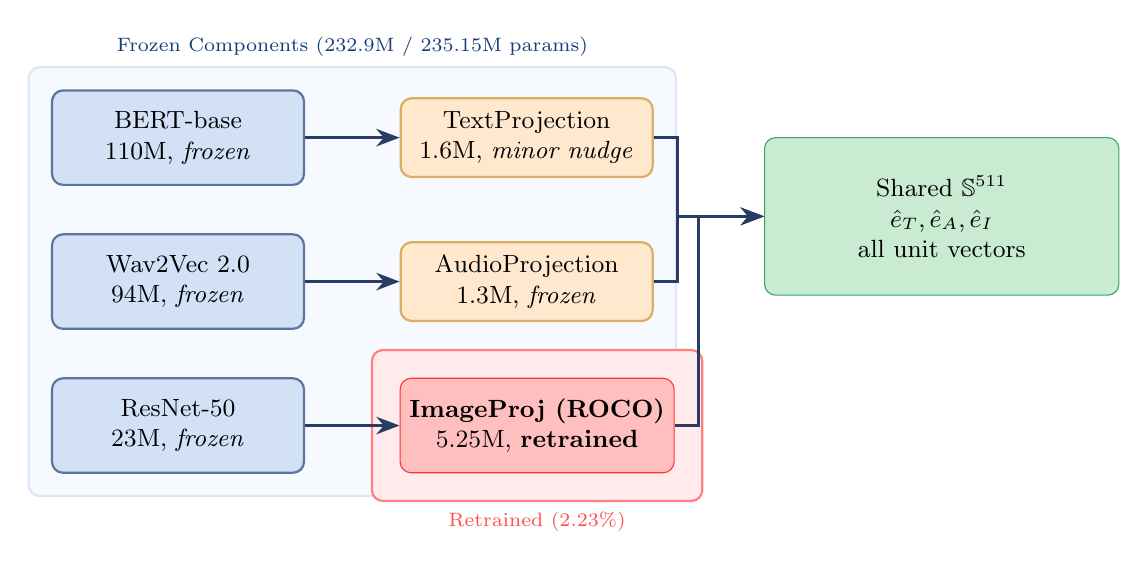
\begin{tikzpicture}[node distance=0.6cm and 1.0cm]
  \node[encnode,minimum width=3.2cm,minimum height=1.2cm] (bert) {BERT-base\\110M, \textit{frozen}};
  \node[encnode,minimum width=3.2cm,minimum height=1.2cm,below=0.6cm of bert] (wav2vec) {Wav2Vec 2.0\\94M, \textit{frozen}};
  \node[encnode,minimum width=3.2cm,minimum height=1.2cm,below=0.6cm of wav2vec] (resnet) {ResNet-50\\23M, \textit{frozen}};

  \node[projnode,minimum width=3.2cm,right=1.2cm of bert] (tproj) {TextProjection\\1.6M, \textit{minor nudge}};
  \node[projnode,minimum width=3.2cm,right=1.2cm of wav2vec] (aproj) {AudioProjection\\1.3M, \textit{frozen}};
  \node[basebox,fill=red!25,draw=red!80,minimum width=3.2cm,minimum height=1.2cm,
        right=1.2cm of resnet] (iproj) {\textbf{ImageProj (ROCO)}\\5.25M, \textbf{retrained}};

  \node[basebox,fill=boxgreen,draw=mintgreen,minimum width=4.5cm,minimum height=2.0cm,
        right=1.4cm of tproj,yshift=-1.0cm] (shared) {Shared $\Sph^{511}$\\$\hat{e}_T, \hat{e}_A, \hat{e}_I$\\all unit vectors};

  \draw[thickarr] (bert)--(tproj); \draw[thickarr] (wav2vec)--(aproj); \draw[thickarr] (resnet)--(iproj);
  \draw[thickarr] (tproj.east) -- ++(0.3,0) |- (shared.west);
  \draw[thickarr] (aproj.east) -- ++(0.3,0) |- (shared.west);
  \draw[thickarr] (iproj.east) -- ++(0.3,0) |- (shared.west);

  \begin{pgfonlayer}{background}
    \node[rectangle,draw=boxblue!80,fill=boxblue!20,rounded corners,thick,
          fit=(bert)(wav2vec)(resnet)(tproj)(aproj),inner sep=8pt,
          label={[font=\scriptsize,color=navyblue]above:Frozen Components (232.9M / 235.15M params)}] {};
    \node[rectangle,draw=red!50,fill=red!8,rounded corners,thick,
          fit=(iproj),inner sep=10pt,
          label={[font=\scriptsize,color=red!70]below:Retrained (2.23\%)}] {};
  \end{pgfonlayer}
\end{tikzpicture}
}
\caption{Pipeline~B surgical domain transfer: only ImageProjection (5.25M/235M params) is retrained for ROCO medical domain.}
\label{fig:pipeline_b}
\end{figure}

\begin{definition}[Dual Loss with Knowledge Distillation]
\[
  \mathcal{L}_{\text{total}} = \mathcal{L}_{\text{align}} + \lambda(t) \cdot \mathcal{L}_{\text{distill}}
\]
\[
  \mathcal{L}_{\text{distill}} = \frac{1}{B}\sum_{i=1}^B \Norm{f_T^{\text{ROCO}}(c_i) - f_T^{\text{M2}}(c_i)}_2^2
\]
where $\lambda(t)$ decays during training to prevent catastrophic forgetting.
\end{definition}

\begin{theorem}[RadLex Seed Coverage Guarantee]
By forcing all RadLex seed terms into $\mathcal{V}_M$, critical imaging terms (e.g.\ \emph{pneumothorax}, \emph{cardiomegaly}) are guaranteed to appear in $\KG_M$ even if they are rare in the ROCO validation split.
\end{theorem}

\begin{algorithm}[H]
\caption{Fine-tune ImageProjection for ROCO Medical Domain}
\label{alg:finetune_roco}
\begin{algorithmic}[1]
\Require ROCO train metadata ($\approx$60K pairs); frozen TextProjection + BERT; frozen ResNet-50
\Ensure \texttt{image\_projection\_roco.pth}
\State Init fresh ImageProjection (random weights)
\State opt$_I \gets$ AdamW(ImageProjection.params, lr=$5\times10^{-4}$)
\State opt$_T \gets$ AdamW(TextProjection.params, lr=$10^{-5}$) \Comment{Nudge only}
\For{epoch $= 1$ to $15$}
  \ForEach{batch $(c_i, \text{img\_path}_i)_{i=1}^{32}$}
    \State $\hat{e}_T \gets \text{L2-norm}(f_T(\text{BERT}(\text{tokenise}(c_i))))$ \quad $[B,512]$
    \State $\hat{e}_I \gets f_\phi(\text{ResNet}(\text{preprocess}(\text{img}_i)))$ \quad $[B,512]$
    \State $\mathcal{L} \gets \mathcal{L}_{\text{InfoNCE}}(\hat{e}_T, \hat{e}_I, \tau{=}0.07) + \lambda(t)\cdot\mathcal{L}_{\text{distill}}$
    \State $\mathcal{L}$.backward(); opt$_I$.step(); opt$_T$.step()
  \EndFor
  \State Save best checkpoint (val loss)
\EndFor
\end{algorithmic}
\end{algorithm}

%%
%% ============================================================
%% PART VIII — TWO-STAGE HYBRID RETRIEVAL
%% ============================================================
%%
\newpage
\section{Two-Stage Hybrid Retrieval Engine}
\label{sec:retrieval}

\subsection{Architecture Overview}

\begin{figure}[H]
\centering
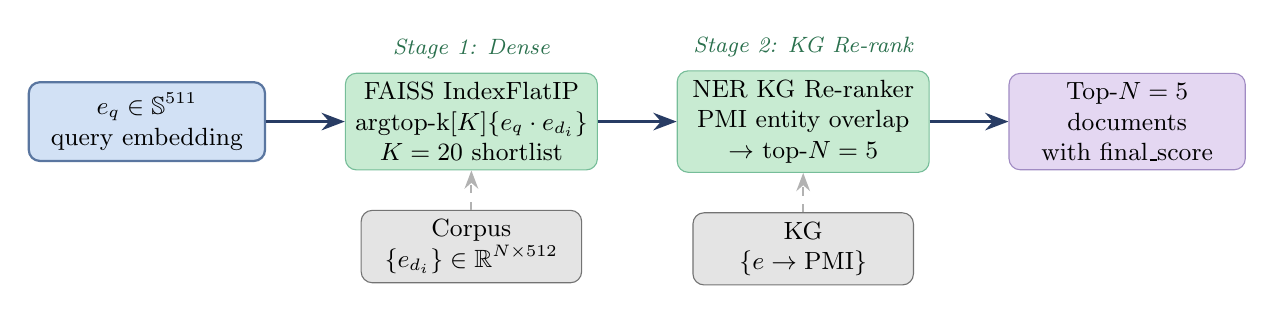
\begin{tikzpicture}[node distance=0.65cm and 1.0cm]
  \node[encnode,minimum width=3.0cm] (qemb) {$e_q \in \Sph^{511}$\\query embedding};
  \node[retnode,right=1.0cm of qemb] (faiss) {FAISS IndexFlatIP\\$\argtopk[K]\{e_q \cdot e_{d_i}\}$\\$K = 20$ shortlist};
  \node[retnode,right=1.0cm of faiss] (kgrank) {NER KG Re-ranker\\PMI entity overlap\\$\to$ top-$N=5$};
  \node[outnode,right=1.0cm of kgrank] (topn) {Top-$N = 5$\\documents\\with final\_score};
  \node[datanode,below=0.5cm of faiss] (corpus) {Corpus\\$\{e_{d_i}\} \in \R^{N \times 512}$};
  \node[datanode,below=0.5cm of kgrank] (kg) {KG\\$\{e \to \text{PMI}\}$};

  \draw[thickarr] (qemb)--(faiss); \draw[thickarr] (faiss)--(kgrank); \draw[thickarr] (kgrank)--(topn);
  \draw[dasharr] (corpus.north)--(faiss.south); \draw[dasharr] (kg.north)--(kgrank.south);
  \node[font=\footnotesize\itshape,color=mintgreen!70!black,above=0.05cm of faiss] {Stage 1: Dense};
  \node[font=\footnotesize\itshape,color=mintgreen!70!black,above=0.05cm of kgrank] {Stage 2: KG Re-rank};
\end{tikzpicture}
\caption{Two-stage hybrid retrieval: dense FAISS search followed by KG PMI re-ranking.}
\label{fig:retrieval}
\end{figure}

\subsection{Stage 1: FAISS Dense Retrieval}

\begin{definition}[FAISS IndexFlatIP]
\[
  \text{dense\_score}(q, d_i) = e_q \cdot e_{d_i} \in [-1,1], \quad
  \mathcal{R}_K = \argtopk_{i}\;(e_q \cdot e_{d_i})
\]
For $N = 69{,}866$ ROCO vectors, exact inner-product search requires $O(N \cdot d) \approx 3.6 \times 10^7$ MACs ($\approx$15\,ms CPU).
\end{definition}

\subsection{Stage 2: PMI Entity Re-ranking}

\begin{algorithm}[H]
\caption{NER KG Re-ranker (Full Algorithm)}
\label{alg:rerank}
\begin{algorithmic}[1]
\Require Shortlist $S = [d_1,\ldots,d_K]$ with dense\_score; query entities $\mathcal{E}_q$; KG; $\alpha = 0.7$
\Ensure Top-$N$ documents with final\_score $\in [0,1]$
\State $s_{\min} \gets \min_i \text{dense\_score}(d_i)$;\; $s_{\max} \gets \max_i \text{dense\_score}(d_i)$;\; $\Delta \gets \max(s_{\max}-s_{\min}, 10^{-6})$
\State $\tilde{s}_{\text{dense}}(d_i) \gets (\text{dense\_score}(d_i) - s_{\min}) / \Delta$
\ForEach{$d_i \in S$}
  \State $\mathcal{E}_{d_i} \gets \text{word-boundary regex extraction from } d_i.\text{text}$
  \State $\text{kg\_raw}(d_i) \gets \sum_{q \in \mathcal{E}_q}\sum_{d \in \mathcal{E}_{d_i}} \text{PMI}(q,d) \cdot \mathbf{1}[q \in \KG,\; d \in \KG[q]]$
\EndFor
\State $m_{\KG} \gets \max_i \text{kg\_raw}(d_i)$;\quad $\tilde{s}_{\KG}(d_i) \gets \text{kg\_raw}(d_i) / \max(m_{\KG}, 10^{-6})$
\ForEach{$d_i \in S$}
  \State $\text{final\_score}(d_i) \gets \alpha \cdot \tilde{s}_{\text{dense}}(d_i) + (1-\alpha)\cdot\tilde{s}_{\KG}(d_i)$
\EndFor
\State \Return $\text{top-}N(S,\; \text{by final\_score desc})$
\end{algorithmic}
\end{algorithm}

\begin{theorem}[Score Bounds]
$\text{final\_score}(d_i) \in [0,1]$ for all $d_i \in S$ under Algorithm~\ref{alg:rerank}, since $\tilde{s}_{\text{dense}}, \tilde{s}_{\KG} \in [0,1]$ by min-max normalisation and $\alpha + (1-\alpha) = 1$.
\end{theorem}

\begin{lemma}[KG Re-ranking Monotonicity]
Since PMI$(a,b) > 0$ is required for every edge, all KG boosts are non-negative. Re-ranking can only improve the rank of semantically related documents; it cannot demote a document below its FAISS-only rank unless another document receives a larger boost.
\end{lemma}

\subsection{Tiered Confidence Guard}

\begin{definition}[Confidence Tier Function]
\[
  \text{tier}(s) = \begin{cases}
    \texttt{full}     & s \ge \tau \\
    \texttt{partial}  & \tau - 0.2 \le s < \tau \\
    \texttt{rejected} & s < \tau - 0.2
  \end{cases}, \quad
  \tau_{\text{general}} = 0.40,\; \tau_{\text{medical}} = 0.55.
\]
\end{definition}

\begin{axiom}[Clinical Safety Constraint]
For clinical domains, false positives carry higher risk than false negatives:
$\tau_{\text{medical}} = \tau_{\text{general}} + 0.15$. The system prefers refusing to answer over generating a plausible but unsafe medical hallucination.
\end{axiom}

\begin{algorithm}[H]
\caption{Full Query Pipeline --- MIVA-KNIGHT Inference}
\label{alg:query}
\begin{algorithmic}[1]
\Require user\_input: TextQuery or AudioQuery; loaded pipeline
\Ensure GeneratorOutput: answer, sources, emotion, audio (optional)
\If{user\_input is AudioQuery}
  \State (transcript, emotion, conf\_emo) $\gets$ AudioEncoder.encode$(a)$
  \If{transcript $= \varnothing$} \Return rejection \EndIf
  \State $(e_q, \mathcal{E}_q, h) \gets$ TextEncoder.encode(transcript)
\Else
  \State $(e_q, \mathcal{E}_q, h) \gets$ TextEncoder.encode$(q)$; emotion $\gets$ ``neutral''
\EndIf
\If{$h \ne \varnothing$} \Call{SwapDomain}{MedicalDomain if $h=$``medical'' else GeneralDomain} \EndIf
\State $(\mathcal{D}^*, s_{\max}) \gets$ HybridRetriever.retrieve$(e_q, \mathcal{E}_q)$
\State tier $\gets$ tier$(s_{\max})$
\If{tier $=$ ``rejected''} \Return \textsc{TieredRejection}(domain.name) \EndIf
\State $g \gets$ GeneratorInput$(q, \text{emotion}, \text{conf\_emo}, \mathcal{D}^*, \Pi, \text{tier})$
\State result $\gets$ Generator.generate$(g)$
\If{TTS enabled} result.audio $\gets$ gTTS.convert(result.answer) \EndIf
\State \Return result
\end{algorithmic}
\end{algorithm}

\begin{theorem}[RAG Faithfulness]
An answer is \emph{faithful} to retrieved context $\mathcal{D}^*$ iff every claim $c$ in the answer can be inferred from some $d_j \in \mathcal{D}^*$. MIVA-KNIGHT enforces faithfulness by: (1) prompting ``Answer using ONLY the retrieved context'', (2) requiring citation, (3) rejecting low-confidence retrievals before any LLM call.
\end{theorem}

%%
%% ============================================================
%% PART IX — PIPELINE C: RAVDESS AUDIO EMOTION
%% ============================================================
%%
\newpage
\section{Pipeline C: RAVDESS Standalone Audio Emotion Recognition}
\label{sec:pipelineC}

\subsection{Wav2Vec 2.0 Backbone}

\begin{definition}[Mean-Pool Audio Embedding]
Let $H = [h_1,\ldots,h_{T'}] \in \R^{T' \times 768}$ be Wav2Vec 2.0's last-layer hidden states for a clip of $T \approx 48{,}000$ samples (3\,s at 16\,kHz):
\[
  e_{\text{wav}} = \frac{1}{T'}\sum_{t=1}^{T'} h_t \in \R^{768}, \quad T' \approx 150.
\]
\end{definition}

\begin{axiom}[Standalone Modality Training]
Audio emotion representations must be learned from audio labels alone, without cross-modal entanglement. The only valid supervisory signal for RAVDESS is the emotion label embedded in each filename.
\end{axiom}

\begin{axiom}[Correct Feature Dimensionality]
Wav2Vec 2.0 base outputs $768$-dimensional hidden states. All components must use $d_{\text{in}} = 768$.
\end{axiom}

\begin{lemma}[Caching Speed-up]
Without caching: $T_{\text{no-cache}} = 1{,}440 \times 30 \times 0.3\,\text{s} \approx 3.6\,\text{h}$.
With caching: $T_{\text{cached}} = 120 + 30 \times 0.3 = 129\,\text{s} \approx 2\,\text{min}$.
Speed-up $\approx 100\times$.
\end{lemma}

\begin{algorithm}[H]
\caption{Extract and Cache RAVDESS Embeddings at 768d}
\label{alg:cache_ravdess}
\begin{algorithmic}[1]
\Require RAVDESS\_DIR; CACHE\_768\_FILE
\Ensure dict: filename $\to$ \{embedding $\in \R^{768}$, emotion, actor\_id, intensity\}
\If{CACHE\_768\_FILE exists} load; \textbf{assert} dim $= 768$; \Return cache \EndIf
\For{each Actor\_XX directory (24 actors)}
  \For{each \texttt{.wav} file}
    \State meta $\gets$ \textsc{ParseRavdessFilename}(filename) \Comment{Emotion from field 3}
    \If{meta is None} \textbf{skip} \EndIf
    \State $e \gets$ Wav2VecEncoder.encode(wav\_path).squeeze(0) \quad $\in \R^{768}$
    \State cache[filename] $\gets$ \{embedding: $e$, emotion: meta.emotion, \ldots\}
  \EndFor
\EndFor
\State torch.save(cache, CACHE\_768\_FILE); del encoder; cuda.empty\_cache()
\end{algorithmic}
\end{algorithm}

\subsection{Supervised Contrastive Loss (SupCon)}

\begin{definition}[Supervised Contrastive Loss]
For batch $B$ with labels $\{y_i\}$, positive set $\mathcal{P}(i) = \{p \ne i : y_p = y_i\}$:
\[
  \boxed{\mathcal{L}_{\text{SupCon}} = \frac{1}{B}\sum_{i=1}^B \frac{-1}{|\mathcal{P}(i)|}
  \sum_{p \in \mathcal{P}(i)} \log\frac{\exp(\hat{e}_i \cdot \hat{e}_p / \tau)}{\sum_{a \ne i} \exp(\hat{e}_i \cdot \hat{e}_a / \tau)}}
\]
with $\tau = 0.07$.
\end{definition}

\begin{table}[H]
\centering
\caption{InfoNCE vs.\ SupCon comparison}
\renewcommand{\arraystretch}{1.2}
\begin{tabular}{lll}
\toprule
\textbf{Property} & \textbf{InfoNCE} & \textbf{SupCon} \\
\midrule
Requires & 2 paired modalities & Emotion labels only \\
Positives/anchor & Exactly 1 & All same-class clips in batch \\
Works without text? & No & Yes \\
Multi-class? & No natural support & Designed for $C$ classes \\
\bottomrule
\end{tabular}
\end{table}

\begin{theorem}[SupCon Random Baseline]
For $B=16$ balanced over $C=8$ classes: $\mathcal{L}_{\text{SupCon}}^{\text{random}} \approx \log(B-1) = \log 15 \approx 2.71$. Target after 30 epochs: $\mathcal{L} < 1.0$.
\end{theorem}

\begin{lemma}[Temperature Effect on Gradient Magnitude]
$\Norm{\partial\mathcal{L}/\partial S_{ij}} \propto 1/\tau$. At $\tau=0.07$, gradients are $\approx 14\times$ larger than at $\tau=1.0$, producing tighter emotion clusters.
\end{lemma}

\begin{algorithm}[H]
\caption{SupCon Loss Computation}
\label{alg:supcon}
\begin{algorithmic}[1]
\Require Embeddings $E \in \R^{B \times D}$; labels $y \in \mathbb{Z}^B$; temperature $\tau$
\Ensure Scalar loss
\State $\hat{E} \gets E / \Norm{E}_2$ (row-wise L2-normalise)
\State $\text{sim} \gets \hat{E}\hat{E}^\top / \tau$ \quad $[B,B]$
\State pos\_mask$[i,j] \gets \mathbf{1}[y_i = y_j \wedge i \ne j]$
\State $\text{sim} \gets \text{sim} - \max(\text{sim}, \text{dim=1})$ \Comment{Log-sum-exp stability}
\State $\text{exp\_sim} \gets \exp(\text{sim}) \odot (1 - I_B)$ \Comment{Exclude self}
\State $\text{log\_prob} \gets \text{sim} - \log(\text{exp\_sim.sum(dim=1)} + \varepsilon)$
\State $n_{\text{pos}} \gets \text{pos\_mask.sum(dim=1)}$; valid $\gets (n_{\text{pos}} > 0)$
\If{valid.sum() $= 0$} \Return 0 \EndIf
\State per\_anchor $\gets -(\text{pos\_mask} \odot \text{log\_prob}).\text{sum(dim=1)}$
\State \Return mean(per\_anchor[valid] / $n_{\text{pos}}$[valid])
\end{algorithmic}
\end{algorithm}

\begin{definition}[Spherical Centroid]
For emotion class $e$ with $N_e$ projected embeddings $\{\hat{a}_i^{(e)}\} \subset \Sph^{511}$:
\[
  \bar{c}_e = \frac{\mu_e}{\Norm{\mu_e}_2}, \quad \mu_e = \frac{1}{N_e}\sum_{i=1}^{N_e}\hat{a}_i^{(e)}.
\]
\end{definition}

\begin{lemma}[Centroid Optimality on $\Sph^{511}$]
The spherical centroid $\bar{c}_e$ minimises $\sum_{i=1}^{N_e} \arccos^2(\hat{a}_i^{(e)} \cdot v)$ over $v \in \Sph^{511}$.
\end{lemma}

\begin{algorithm}[H]
\caption{Emotion Accuracy Evaluation via Centroid Nearest-Neighbour}
\label{alg:centroid_eval}
\begin{algorithmic}[1]
\Require audio\_proj $f_\theta$; data loader
\Ensure overall accuracy; per-emotion dict; centroids $[C, 512]$
\State audio\_proj.eval()
\State $E \gets \text{cat}([f_\theta(E_b) \text{ for each batch}])$ \quad $[N, 512]$
\State $Y \gets \text{cat}([y_b \text{ for each batch}])$ \quad $[N]$
\For{$c = 0$ to $C-1$}
  \State $\bar{c}_c \gets \text{L2-norm}(E[Y{=}c].\text{mean(dim=0)})$
\EndFor
\State $C_{\text{mat}} \gets \text{stack}(\bar{c}_0,\ldots,\bar{c}_{C-1})$ \quad $[C, 512]$
\State predicted $\gets \argmax(E \cdot C_{\text{mat}}^\top, \text{dim=1})$
\State accuracy $\gets \text{mean}(\text{predicted} = Y)$
\State \Return accuracy, per-emotion breakdown, $C_{\text{mat}}$
\end{algorithmic}
\end{algorithm}

%%
%% ============================================================
%% PART X — PIPELINE D: CREMA-D AUDIO-VISUAL EMOTION
%% ============================================================
%%
\newpage
\section{Pipeline D: CREMA-D Audio-Visual Emotion Recognition}
\label{sec:pipelineD}

\subsection{Overview and Three-Phase Training Strategy}

Pipeline~D extends emotion recognition to the CREMA-D dataset (7,442 clips, 91 actors, 6 emotions) using two frozen backbones: Wav2Vec 2.0 (94M, audio) and ResNet-50 (23M, middle frame video). Only projection heads ($\approx$3.6M params) train.

\begin{figure}[H]
\centering
\begin{adjustbox}{max width=\textwidth}
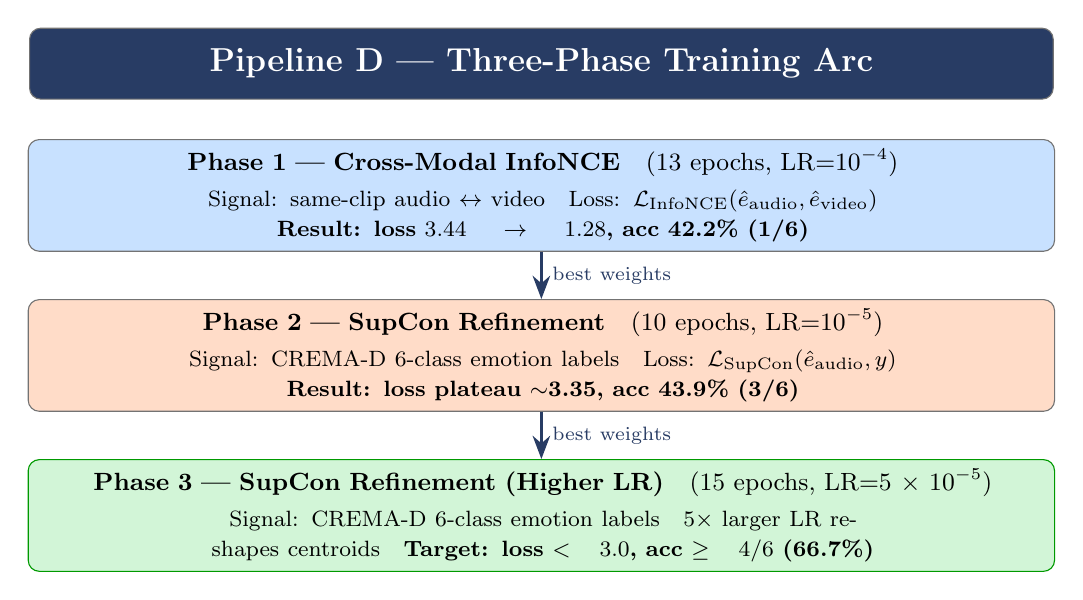
\begin{tikzpicture}[node distance=0.7cm]
  \node[basebox,fill=cDark,text=white,minimum width=13cm,minimum height=0.9cm] (hdr)
      {\large\bfseries Pipeline D --- Three-Phase Training Arc};
  \node[basebox,fill=cPhase1,minimum width=13cm,minimum height=1.2cm,text width=12.8cm,
        below=0.5cm of hdr] (p1)
      {\textbf{Phase 1 --- Cross-Modal InfoNCE}\quad(13 epochs, LR=$10^{-4}$)\\[2pt]
       \footnotesize Signal: same-clip audio $\leftrightarrow$ video\quad
       Loss: $\mathcal{L}_{\text{InfoNCE}}(\hat{e}_{\text{audio}}, \hat{e}_{\text{video}})$\quad
       \textbf{Result: loss $3.44\to1.28$, acc 42.2\% (1/6)}};
  \node[basebox,fill=cPhase2,minimum width=13cm,minimum height=1.2cm,text width=12.8cm,
        below=0.6cm of p1] (p2)
      {\textbf{Phase 2 --- SupCon Refinement}\quad(10 epochs, LR=$10^{-5}$)\\[2pt]
       \footnotesize Signal: CREMA-D 6-class emotion labels\quad
       Loss: $\mathcal{L}_{\text{SupCon}}(\hat{e}_{\text{audio}}, y)$\quad
       \textbf{Result: loss plateau $\sim$3.35, acc 43.9\% (3/6)}};
  \node[basebox,fill=cPhase3,draw=green!60!black,minimum width=13cm,minimum height=1.2cm,
        text width=12.8cm,below=0.6cm of p2] (p3)
      {\textbf{Phase 3 --- SupCon Refinement (Higher LR)}\quad(15 epochs, LR=$5\times10^{-5}$)\\[2pt]
       \footnotesize Signal: CREMA-D 6-class emotion labels\quad
       $5\times$ larger LR reshapes centroids\quad
       \textbf{Target: loss $< 3.0$, acc $\geq 4/6$ (66.7\%)}};

  \draw[thickarr] (p1.south) -- (p2.north) node[midway,right,font=\scriptsize]{best weights};
  \draw[thickarr] (p2.south) -- (p3.north) node[midway,right,font=\scriptsize]{best weights};
\end{tikzpicture}
\end{adjustbox}
\caption{Pipeline D three-phase training arc: InfoNCE alignment $\to$ SupCon cluster sharpening $\to$ higher-LR SupCon refinement.}
\label{fig:pipeline_d_phases}
\end{figure}

\begin{definition}[VideoFrameProjection $f_\phi^{\text{video}}$]
Let $I \in \R^{3 \times 224 \times 224}$ be an ImageNet-normalised middle frame.
\[
  f_\phi^{\text{video}}(I) = \text{L2-norm}\!\left(\LN_{512}(W_4 \cdot \GELU(\LN_{1024}(W_3 \cdot r(I) + b_3)) + b_4)\right)
\]
where $r(I) = \text{ResNet50}(I) \in \R^{2048}$ (frozen), $W_3 \in \R^{1024 \times 2048}$, $W_4 \in \R^{512 \times 1024}$. Trainable: $\approx$2.63\,M parameters.
\end{definition}

\begin{theorem}[Peak Expression Frame]
The middle frame of a short acted-emotion clip ($\le 3$\,s) maximises the probability of capturing the peak facial action unit configuration, as actors complete their ramp-up in the first half and relax in the final quarter.
\end{theorem}

\begin{algorithm}[H]
\caption{CREMA-D Middle-Frame Extraction}
\label{alg:frame_extract}
\begin{algorithmic}[1]
\Require mp4\_path; FRAME\_TRANSFORM (Resize224 $\to$ CentCrop $\to$ ToTensor $\to$ ImageNetNorm)
\Ensure $(f, \text{success})$, $f \in \R^{3 \times 224 \times 224}$
\State cap $\gets$ cv2.VideoCapture(mp4\_path)
\If{not cap.isOpened()} \Return (GrayFallback, False) \EndIf
\State $N \gets$ cap.get(CAP\_PROP\_FRAME\_COUNT)
\State cap.set(CAP\_PROP\_POS\_FRAMES, $\max(0, \lfloor N/2 \rfloor)$) \Comment{Seek to midpoint}
\State (ret, frame) $\gets$ cap.read(); cap.release()
\If{not ret} \Return (GrayFallback, False) \EndIf
\State rgb $\gets$ cv2.cvtColor(frame, COLOR\_BGR2RGB)
\State $f \gets$ FRAME\_TRANSFORM(Image.fromarray(rgb))
\State \Return $(f, \text{True})$
\end{algorithmic}
\end{algorithm}

\begin{theorem}[Phase 2 LR Insufficiency]
Phase 2's LR $= 10^{-5}$ was insufficient to meaningfully reposition centroids. Weight update per step: $\Delta_{\text{Phase 2}} \approx 10^{-5} \times 12.4 \approx 1.24 \times 10^{-4}$ (marginal). Phase~3: $\Delta_{\text{Phase 3}} \approx 5 \times 10^{-5} \times 12.4 \approx 6.2 \times 10^{-4}$ (meaningful), while preserving InfoNCE geometry.
\end{theorem}

\begin{lemma}[SupCon Cluster Geometry]
Under SupCon minimisation, the optimal geometry concentrates class $c$ at $\bar{c}_c = \mu_c/\Norm{\mu_c}$, with inter-class angle approaching $\theta_{cc'} = \arccos(-1/(K-1))$, $K=6$ --- the maximum-separation packing (regular simplex inscribed in $\Sph^{511}$).
\end{lemma}

\begin{algorithm}[H]
\caption{Stage 1: Cross-Modal InfoNCE Training (Pipeline D)}
\label{alg:stage1_d}
\begin{algorithmic}[1]
\Require audio\_proj (warm-start from Pipeline~C); video\_proj (random init); $E = 13$
\For{$e = 0$ to $E-1$}
  \ForEach{$(e_{\text{wav}}^{[B,768]}, \text{frame}^{[B,3,224,224]}, \text{labels}^{[B]})$ in loader}
    \State $\hat{e}_A \gets \text{audio\_proj}(e_{\text{wav}}.\text{to(device)})$ \quad $[B,512]$
    \State $\hat{e}_V \gets \text{video\_proj}(\text{frame}.\text{to(device)})$ \quad (ResNet inside no\_grad)
    \State $\mathcal{L} \gets \mathcal{L}_{\text{InfoNCE}}(\hat{e}_A, \hat{e}_V, \tau{=}0.07)$
    \State optimizer.zero\_grad(); $\mathcal{L}$.backward(); ClipGradNorm(params, $c = 1.0$)
    \State optimizer.step(); scheduler.step()
  \EndFor
  \State acc $\gets$ \textsc{EvaluateAccuracy}()
  \If{acc $>$ best\_acc} save best\_audio\_sd, best\_video\_sd \EndIf
\EndFor
\end{algorithmic}
\end{algorithm}

%%
%% ============================================================
%% PART XI — PIPELINE E: CMU-MOSI SENTIMENT FUSION
%% ============================================================
%%
\newpage
\section{Pipeline E: CMU-MOSI Multimodal Sentiment Fusion}
\label{sec:pipelineE}

\subsection{Overview}

Pipeline~E processes three concurrent data streams from the CMU-MOSI corpus (2,199 video opinion segments, 93 YouTube videos, sentiment $y \in [-3, +3]$) using a cross-modal Transformer encoder. This is the fullest realisation of the model-based fusion taxonomy cell.

\begin{figure}[H]
\centering
\resizebox{\textwidth}{!}{%
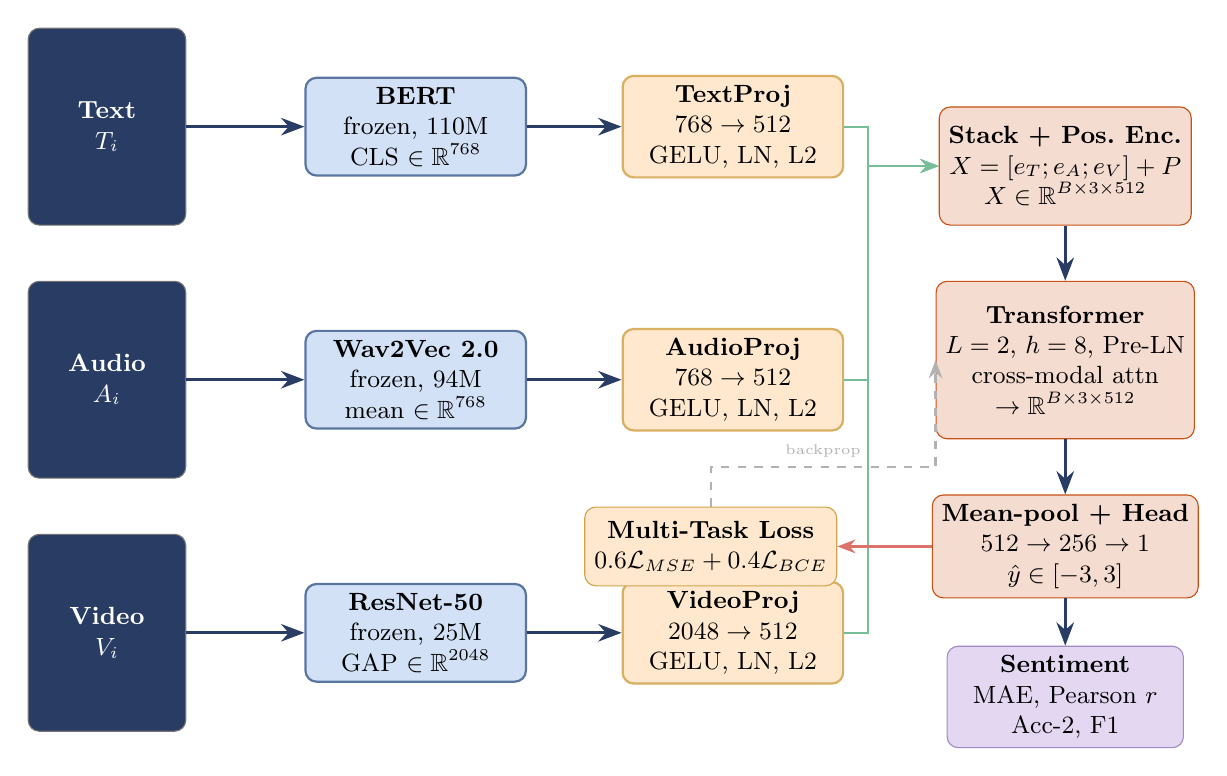
\begin{tikzpicture}[node distance=1.0cm and 1.3cm]
  \node[inputnode,minimum width=2.0cm,minimum height=2.5cm] (textIn) at (0,0) {\textbf{Text}\\$T_i$};
  \node[inputnode,minimum width=2.0cm,minimum height=2.5cm,below=0.7cm of textIn] (audioIn) {\textbf{Audio}\\$A_i$};
  \node[inputnode,minimum width=2.0cm,minimum height=2.5cm,below=0.7cm of audioIn] (videoIn) {\textbf{Video}\\$V_i$};

  \node[encnode,right=1.5cm of textIn,minimum width=2.8cm] (bert2) {\textbf{BERT}\\frozen, 110M\\CLS $\in \R^{768}$};
  \node[encnode,right=1.5cm of audioIn,minimum width=2.8cm] (wav2) {\textbf{Wav2Vec 2.0}\\frozen, 94M\\mean $\in \R^{768}$};
  \node[encnode,right=1.5cm of videoIn,minimum width=2.8cm] (res2) {\textbf{ResNet-50}\\frozen, 25M\\GAP $\in \R^{2048}$};

  \node[projnode,right=1.2cm of bert2,minimum width=2.8cm] (tp) {\textbf{TextProj}\\$768\to512$\\GELU, LN, L2};
  \node[projnode,right=1.2cm of wav2,minimum width=2.8cm] (ap) {\textbf{AudioProj}\\$768\to512$\\GELU, LN, L2};
  \node[projnode,right=1.2cm of res2,minimum width=2.8cm] (vp) {\textbf{VideoProj}\\$2048\to512$\\GELU, LN, L2};

  \node[basebox,fill=fusioncolor!20,draw=fusioncolor,minimum width=3.2cm,minimum height=1.5cm,
        right=1.2cm of tp,yshift=-0.5cm] (stack)
      {\textbf{Stack + Pos.\ Enc.}\\$X = [e_T;e_A;e_V]+P$\\$X \in \R^{B \times 3 \times 512}$};

  \node[basebox,fill=fusioncolor!20,draw=fusioncolor,minimum width=3.2cm,minimum height=2.0cm,
        below=0.7cm of stack] (transf)
      {\textbf{Transformer}\\$L=2$, $h=8$, Pre-LN\\cross-modal attn\\$\to \R^{B\times3\times512}$};

  \node[basebox,fill=fusioncolor!20,draw=fusioncolor,minimum width=3.2cm,
        below=0.7cm of transf] (reg)
      {\textbf{Mean-pool + Head}\\$512\to256\to1$\\$\hat{y} \in [-3,3]$};

  \node[lossnode,left=1.2cm of reg] (loss2) {\textbf{Multi-Task Loss}\\$0.6\mathcal{L}_{MSE}+0.4\mathcal{L}_{BCE}$};
  \node[outnode,below=0.6cm of reg] (out2) {\textbf{Sentiment}\\MAE, Pearson $r$\\Acc-2, F1};

  \draw[thickarr] (textIn)--(bert2); \draw[thickarr] (audioIn)--(wav2); \draw[thickarr] (videoIn)--(res2);
  \draw[thickarr] (bert2)--(tp); \draw[thickarr] (wav2)--(ap); \draw[thickarr] (res2)--(vp);
  \draw[greenarr] (tp.east) -- ++(0.3,0) |- (stack.west);
  \draw[greenarr] (ap.east) -- ++(0.3,0) |- (stack.west);
  \draw[greenarr] (vp.east) -- ++(0.3,0) |- (stack.west);
  \draw[thickarr] (stack)--(transf);
  \draw[thickarr] (transf)--(reg);
  \draw[redarr] (reg)--(loss2);
  \draw[dasharr] (loss2.north) -- ++(0,0.5) -| (transf.west) node[near start,above,font=\tiny]{backprop};
  \draw[thickarr] (reg)--(out2);
\end{tikzpicture}
}
\caption{Pipeline~E: three-modality fusion for CMU-MOSI sentiment analysis using a cross-modal Transformer.}
\label{fig:pipeline_e}
\end{figure}

\subsection{MultimodalFusionTransformer}

\begin{definition}[MultimodalFusionTransformer]
$\pi_\theta : \R^{512} \times \R^{512} \times \R^{512} \to \R$ consists of:
(1) learnable positional encodings $P \in \R^{3 \times 512}$; (2) $L=2$-layer Pre-LN Transformer with $h=8$ attention heads, $d_{ff}=1024$; (3) mean-pool over 3 tokens; (4) regression head: Linear$(512\!\to\!256)\to\GELU\to\text{Dropout}(0.1)\to$Linear$(256\!\to\!1)$.
\end{definition}

\begin{theorem}[Scaled Dot-Product Attention]
$\text{Attn}(Q,K,V) = \softmax\!\left(\frac{QK^\top}{\sqrt{d_k}}\right)V$. The $1/\sqrt{d_k}$ factor prevents dot products from growing large and pushing softmax to saturation.
\end{theorem}

\begin{axiom}[Pre-LN Stability]
Pre-LN architecture: $x' = x + \text{Attn}(\LN(x))$, $x'' = x' + \text{FFN}(\LN(x'))$. Provides more stable gradients during early training compared to Post-LN, because the residual pathway preserves gradient magnitude.
\end{axiom}

\begin{algorithm}[H]
\caption{MultimodalFusionTransformer.forward}
\label{alg:fusion_forward}
\begin{algorithmic}[1]
\Require $\hat{e}_T, \hat{e}_A, \hat{e}_V \in \R^{B \times 512}$; parameters $\theta$
\Ensure Sentiment scores $\hat{y} \in \R^B$
\State $X \gets \text{stack}([\hat{e}_T, \hat{e}_A, \hat{e}_V], \text{dim}=1) \in \R^{B \times 3 \times 512}$
\State $X \gets X + P$ \Comment{Learnable modality positional encodings}
\For{$\ell = 1$ to $L=2$}
  \State $X \gets X + \MHA(\LN(X))$ \Comment{Pre-LN self-attention}
  \State $X \gets X + \text{FFN}(\LN(X))$ \Comment{Pre-LN feed-forward}
\EndFor
\State $\bar{x} \gets X.\text{mean(dim=1)} \in \R^{B \times 512}$
\State $z \gets \GELU(W_1 \bar{x} + b_1) \in \R^{B \times 256}$
\State $z \gets \text{Dropout}(z, p=0.1)$
\State $\hat{y} \gets W_2 z + b_2 \in \R^B$
\State \Return $\hat{y}$
\end{algorithmic}
\end{algorithm}

\begin{algorithm}[H]
\caption{Full Training Loop --- Pipeline E (20 Epochs, Best-Model Tracking)}
\label{alg:training_e}
\begin{algorithmic}[1]
\Require Model $\pi_\theta$; train/valid loaders; AdamW optimizer; cosine warmup scheduler; $E=20$
\Ensure Best model state $\theta^*$
\State best\_mae $\gets \infty$; $\theta^* \gets$ None
\For{$e = 0$ to $E-1$}
  \ForEach{batch $(T, A, V, y, b)$ in train\_loader}
    \State $\hat{y} \gets \pi_\theta(T, A, V)$
    \State $\mathcal{L} \gets 0.6\mathcal{L}_{\text{MSE}}(\hat{y},y) + 0.4\mathcal{L}_{\text{BCE}}(\hat{y},b)$
    \State optimizer.zero\_grad(); $\mathcal{L}$.backward()
    \State clip\_grad\_norm$(\theta, c=1.0)$; optimizer.step(); scheduler.step()
  \EndFor
  \State MAE$_\text{val} \gets$ Evaluate(valid\_loader)
  \If{MAE$_\text{val} < $ best\_mae}
    \State best\_mae $\gets$ MAE$_\text{val}$; $\theta^* \gets \pi_\theta.\text{state\_dict().clone()}$
  \EndIf
  \State torch.save(checkpoint, path)
\EndFor
\State \Return $\theta^*$ \Comment{Best: epoch 17, val MAE $= 0.7238$}
\end{algorithmic}
\end{algorithm}

%%
%% --- Pipeline E: comprehensive notebook integration (thesis-grade) ---
%%
\subsection{Strict multimodal protocol, pseudo-labels, and embedding cache}
\label{sec:pipelineE_strict}

The comprehensive notebook enforces a \textbf{strict multimodal cohort}: a segment is admitted only if both \path{Audio/WAV_16000/Segmented/{vid}_{seg}.wav} and \path{Video/Segmented/{vid}_{seg}.mp4} exist. This matches the engineering requirement that Pipeline~E training never relies on synthetic silence or gray-frame video placeholders.

\begin{axiom}[Strict Multimodal Integrity (Pipeline~E)]
\label{ax:strict_mosi}
Let $\mathcal{U}$ be the set of segment IDs in the CMU-MOSI standard video-level split. The training population is $\mathcal{U}^\star = \{u \in \mathcal{U} : \text{file}(\text{audio},u) \wedge \text{file}(\text{video},u)\}$. All reported Pipeline~E statistics are computed on $\mathcal{U}^\star$ unless explicitly ablated.
\end{axiom}

\begin{definition}[TextBlob pseudo-label on $[-3,+3]$]
When gold sentiment annotations are unavailable, each transcript line yields
\[
  y \;=\; \mathrm{clip}\bigl(3 \cdot \mathrm{polarity}_{\text{TB}}(\text{text}),\,-3,\,+3\bigr),\qquad
  b \;=\; \mathbf{1}[y > 0],
\]
where $\mathrm{polarity}_{\text{TB}} \in [-1,1]$ is TextBlob's rule-based polarity.
\end{definition}

\begin{remark}[Impact on Acc-2]
Pseudo-label noise primarily hurts \textbf{binary} agreement (Acc-2) while regression MAE can remain competitive with strong frozen encoders --- consistent with reported MAE vs.\ MulT/MISA comparisons in the notebook.
\end{remark}

\begin{algorithm}[H]
\caption{Strict CMU-MOSI sample list and multimodal cache (Pipeline~E notebook)}
\label{alg:mosi_cache_strict}
\begin{algorithmic}[1]
\Require \textsc{Transcript/Segmented/*.annotprocessed}; \textsc{Audio/}; \textsc{Video/}; train/valid/test video ID lists
\Ensure Cache dictionary $\mathcal{C}: \text{segment\_id} \mapsto \{\hat{e}_T,\hat{e}_A,\hat{e}_V,y,b,\texttt{split},\texttt{text},p_{\text{wav}},p_{\text{mp4}}\}$
\State $\mathcal{S} \gets \emptyset$
\ForEach{file $f = \texttt{\{vid\}.annotprocessed}$}
  \If{$\texttt{vid} \notin$ standard split} \textbf{continue} \EndIf
  \ForEach{line with $\texttt{seg}\_\texttt{DELIM}\_\texttt{text}$}
    \If{$\neg$ \textsc{Exists}$(\texttt{wav}(\texttt{vid},\texttt{seg}))$ \textbf{or} $\neg$ \textsc{Exists}$(\texttt{mp4}(\texttt{vid},\texttt{seg}))$} \textbf{continue} \EndIf
    \State append segment metadata (text, paths, $y$, $b$, split) to $\mathcal{S}$
  \EndFor
\EndFor
\If{$\mathcal{S} = \emptyset$} \textbf{error:} no multimodal segments \EndIf
\If{cache file exists with $> 100$ entries} \State \Return loaded $\mathcal{C}$ \EndIf
\ForEach{$s \in \mathcal{S}$}
  \State $\hat{e}_T \gets \textsc{EncText}(s.\text{text})$ \Comment{BERT [CLS] $\to$ TextProj $\to \Sph^{511}$}
  \State $\hat{e}_A \gets \textsc{EncAudio}(s.p_{\text{wav}})$ \Comment{Wav2Vec mean-pool $\to$ AudioProj}
  \State $\hat{e}_V \gets \textsc{EncVideo}(s.p_{\text{mp4}})$ \Comment{ResNet middle frame $\to$ VideoProj}
  \State store all fields in $\mathcal{C}[s.\text{id}]$
\EndFor
\State \Return $\mathcal{C}$
\end{algorithmic}
\end{algorithm}

\subsection{Empirical five-challenge suite on CMU-MOSI}
\label{sec:pipelineE_challenges}

The notebook instantiates the taxonomy of \S\ref{sec:fivechallenges} \emph{on the same cached embeddings} as the fusion model, yielding reproducible diagnostics beyond raw test MAE.

\begin{theorem}[Monotone Step Sentiment Labels (inference)]
\label{thm:step_labels}
The \texttt{MultimodalFusionDetector} maps $\hat{y} \in \R$ to one of seven ordered sentiment classes via a fixed threshold ladder; the map is monotone in $\hat{y}$ (piecewise-constant inverse of a monotone partition of $\R$).
\end{theorem}

\begin{lemma}[Random InfoNCE baseline]
For symmetric InfoNCE with in-batch negatives, $\mathbb{E}[\mathcal{L}_{\mathrm{NCE}}] \approx \log B$ at random initialization, $B$ batch size.
\end{lemma}

\begin{algorithm}[H]
\caption{Challenge suite C1--C5 + fusion metrics (test split, notebook)}
\label{alg:pipeline_e_challenges}
\begin{algorithmic}[1]
\Require Cache $\mathcal{C}$; trained $\pi_\theta$; test keys $\mathcal{K}_{\text{test}}$
\State \textbf{C1 (Representation):} On $\mathcal{K}' \subseteq \mathcal{K}_{\text{test}}$, compute $\mathrm{P@}k$, MRR for text$\to$audio retrieval with diagonal relevance; optional $\mathcal{L}_{\mathrm{NCE}}$ on batches of $(\hat{e}_T,\hat{e}_A)$.
\State \textbf{C2 (Translation):} For $k \leq |\mathcal{K}_{\text{test}}|$, run Whisper \texttt{base} on real \texttt{.wav}; reference text from $\mathcal{C}[\cdot].\texttt{text}$, then \texttt{all\_samples}, else parse \texttt{.annotprocessed}. Report mean WER, score $1-\mathrm{WER}$.
\State \textbf{C3 (Fusion):} Evaluate $\pi_\theta$ on test loader: MAE, Pearson $r$, Acc-2 $(\mathrm{sign}(\hat{y})=\mathrm{sign}(y))$, weighted F1.
\State \textbf{C4 (Co-learning):} Compare $\mathbb{E}[\langle \hat{e}_T,\hat{e}_A\rangle]$ same-segment vs.\ shuffled audio on train subset; report gap.
\State \textbf{C5 (Alignment):} Same-segment vs.\ permuted-audio cosine gap; optional soft-attention and DTW cost on short embedding sequences.
\State \Return metric dictionary for dashboard
\end{algorithmic}
\end{algorithm}

\begin{figure}[H]
\centering
\resizebox{0.98\textwidth}{!}{%
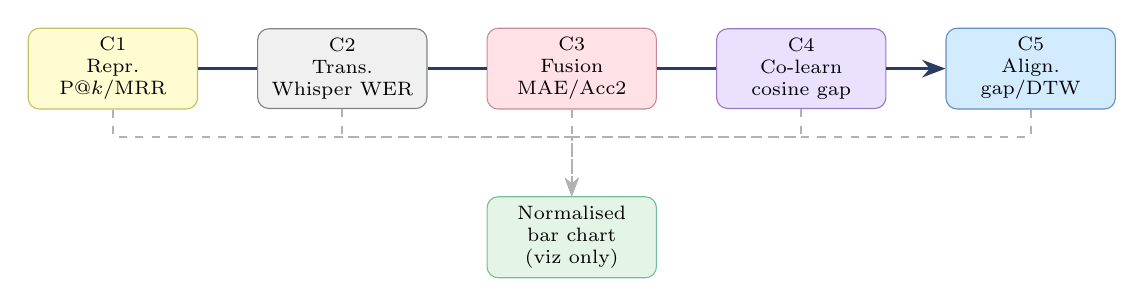
\begin{tikzpicture}[
  node distance=0.55cm and 0.75cm,
  ch/.style={basebox,minimum width=2.15cm,minimum height=0.95cm,font=\scriptsize},
]
  \node[ch,fill=reprYellow,draw=reprBorder] (c1) {C1\\Repr.\\P@$k$/MRR};
  \node[ch,fill=transGray,draw=transBorder,right=of c1] (c2) {C2\\Trans.\\Whisper WER};
  \node[ch,fill=fuseRose,draw=fuseBorder,right=of c2] (c3) {C3\\Fusion\\MAE/Acc2};
  \node[ch,fill=coLearnPurple,draw=coLearnBorder,right=of c3] (c4) {C4\\Co-learn\\cosine gap};
  \node[ch,fill=alignBlue,draw=alignBorder,right=of c4] (c5) {C5\\Align.\\gap/DTW};
  \node[ch,fill=boxgreen!50,draw=mintgreen!70,below=1.1cm of c3] (dash) {Normalised\\bar chart\\(viz only)};
  \draw[thickarr] (c1)--(c2)--(c3)--(c4)--(c5);
  \foreach \x in {c1,c2,c3,c4,c5} \draw[dasharr] (\x.south) -- ++(0,-0.35) -| (dash.north);
\end{tikzpicture}%
}
\caption{Pipeline~E Part~II: five multimodal challenges evaluated on shared CMU-MOSI cache embeddings; optional dashboard compares \emph{normalised} scalars (C1: P@1; C2: $1-$WER; C3: Acc-2; C4/C5: clipped alignment gaps) for visualisation only --- not a single commensurate ``accuracy''.}
\label{fig:pipeline_e_challenges_flow}
\end{figure}

\subsection{Knowledge graph and hybrid RAG restricted to CMU-MOSI transcripts}
\label{sec:pipelineE_mosi_rag}

The notebook constructs a \textbf{corpus-specific} knowledge graph $\KG_{\text{MOSI}}$ from \emph{training-split} transcript strings using the same co-occurrence edge pattern as Month~1 (\texttt{appears\_with}) and a 2-hop DFS neighbour expansion (cf.\ Algorithms~\ref{alg:kg_build}--\ref{alg:kgdfs}). Dense retrieval uses a separate BERT mean-pooled encoder and FAISS \texttt{IndexFlatIP} over training documents $d_i$ (each a full transcript line).

\begin{definition}[Hybrid score on MOSI corpus]
Let $s_{\text{dense}}(q,d_i)$ be inner product similarity between L2-normalised BERT vectors (equivalently cosine). Let $b_{\KG}(q,d_i)$ be the maximum $1/(h{+}1)$ boost from any query entity's $h$-hop neighbour lemma appearing in $d_i$. Then
\begin{equation}
  s_{\text{hyb}}(q,d_i) \;=\; \alpha_{\text{E}}\, s_{\text{dense}}(q,d_i) + (1-\alpha_{\text{E}})\, b_{\KG}(q,d_i),
  \qquad \alpha_{\text{E}} = 0.6.
\end{equation}
\end{definition}

\begin{remark}[$\alpha$ vs.\ global hybrid RAG]
The global assistant (\S\ref{sec:retrieval}) uses $\alpha=0.7$ in some expositions; the MOSI notebook uses $\alpha_{\text{E}}=0.6$ to match the annotated training notebook's dense/graph blend. Both are convex combinations preserving a valid score mixture.
\end{remark}

\begin{algorithm}[H]
\caption{Hybrid retrieval over CMU-MOSI training transcripts (notebook)}
\label{alg:mosi_hybrid_rag}
\begin{algorithmic}[1]
\Require Query string $q$; FAISS index over $\{\phi(d_i)\}$; $\KG_{\text{MOSI}}$; $\alpha_{\text{E}}$; shortlist multiplier $m$
\State $\mathbf{q} \gets \mathrm{L2Norm}(\text{BERT-mean}(q))$
\State $\mathcal{I} \gets \argtopk[m\cdot K]$ by $\mathbf{q}^\top \phi(d_i)$ \Comment{FAISS inner product}
\State extract query entities $\mathcal{E}_q$ by lemma overlap with $\KG_{\text{MOSI}}.\mathcal{V}$
\ForEach{$i \in \mathcal{I}$}
  \State $b_i \gets \textsc{GraphBoost}(d_i, \mathcal{E}_q, \KG_{\text{MOSI}})$ \Comment{max over neighbours, hop decay}
  \State $s_i \gets \alpha_{\text{E}} \cdot s_{\text{dense},i} + (1-\alpha_{\text{E}}) \cdot b_i$
\EndFor
\State \Return top-$K$ documents by $s_i$
\end{algorithmic}
\end{algorithm}

\begin{figure}[H]
\centering
\resizebox{0.98\textwidth}{!}{%
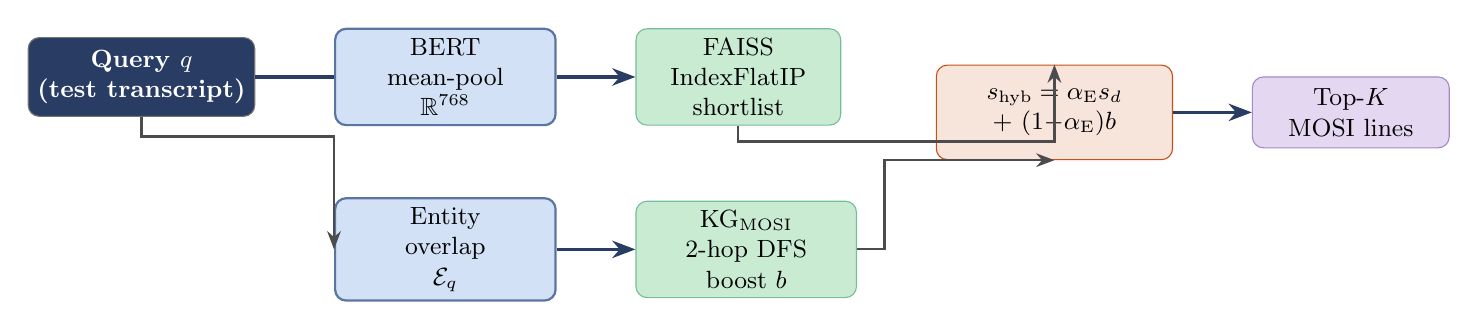
\begin{tikzpicture}[node distance=0.7cm and 1.0cm]
  \node[inputnode,minimum width=2.4cm] (q) {Query $q$\\(test transcript)};
  \node[encnode,right=of q,minimum width=2.8cm] (bert) {BERT\\mean-pool\\$\R^{768}$};
  \node[retnode,right=of bert,minimum width=2.6cm] (fa) {FAISS\\IndexFlatIP\\shortlist};
  \node[encnode,below=0.9cm of bert,minimum width=2.8cm] (ent) {Entity\\overlap\\$\mathcal{E}_q$};
  \node[retnode,right=of ent,minimum width=2.8cm] (kg) {KG$_{\text{MOSI}}$\\2-hop DFS\\boost $b$};
  \node[basebox,fill=fusioncolor!15,draw=fusioncolor,right=1.2cm of fa,yshift=-0.45cm,minimum width=3.0cm,minimum height=1.2cm] (mix) {$s_{\text{hyb}}=\alpha_{\text{E}} s_d$\\$+\ (1{-}\alpha_{\text{E}}) b$};
  \node[outnode,right=of mix,minimum width=2.5cm] (out) {Top-$K$\\MOSI lines};
  \draw[thickarr] (q)--(bert)--(fa);
  \draw[arr] (q.south)--++(0,-0.25)-|(ent.west);
  \draw[thickarr] (ent)--(kg);
  \draw[arr] (fa.south)--++(0,-0.2)-|(mix.north);
  \draw[arr] (kg.east)--++(0.35,0)|-(mix.south);
  \draw[thickarr] (mix)--(out);
\end{tikzpicture}%
}
\caption{Hybrid RAG \emph{inside} the CMU-MOSI training corpus: dense BERT--FAISS shortlisting plus graph boost from co-occurrence entities (notebook Part~II).}
\label{fig:mosi_hybrid_rag}
\end{figure}

\subsection{Publication roadmap: from thesis to competitive venues}
\label{sec:pipelineE_publication}

\begin{itemize}[nosep]
  \item \textbf{NeurIPS / ICML / ICLR:} emphasise \emph{strict multimodal integrity}, pseudo-label bias analysis, and the five-challenge evaluation as a \textbf{diagnostic suite} for multimodal sentiment; contrastive retrieval (C1) + the InfoNCE random-baseline lemma.
  \item \textbf{CVPR / ICCV:} foreground middle-frame video protocol, strict failure modes (corrupt \texttt{.mp4}), and optional visual quality ablations.
  \item \textbf{Interspeech / ICASSP:} foreground Whisper WER (C2), Wav2Vec frozen backbone, and audio--text alignment gaps (C5).
  \item \textbf{ACL / EMNLP:} foreground $\KG_{\text{MOSI}}$ hybrid retrieval over \emph{spoken-content transcripts} as a lightweight domain adaptation of HybridRAG-style systems.
\end{itemize}

\begin{remark}[Condensing to an IEEE-style article]
A camera-ready version merges \S\ref{sec:pipelineE_strict}--\ref{sec:pipelineE_mosi_rag} into: (i) Problem + strict cohort, (ii) Method (cache + Pre-LN fusion), (iii) Five-challenge evaluation table + hybrid transcript retrieval, (iv) Limitations (TextBlob, middle frame), (v) Ethics. Figures~\ref{fig:pipeline_e}--\ref{fig:mosi_hybrid_rag} provide the main architecture + diagnostic flow.
\end{remark}

%%
%% ============================================================
%% PART XII — FULL MIVA-KNIGHT SYSTEM PIPELINE
%% ============================================================
%%
\newpage
\section{Full MIVA-KNIGHT System Pipeline}
\label{sec:system}

\begin{figure}[H]
\centering
\resizebox{\textwidth}{!}{%
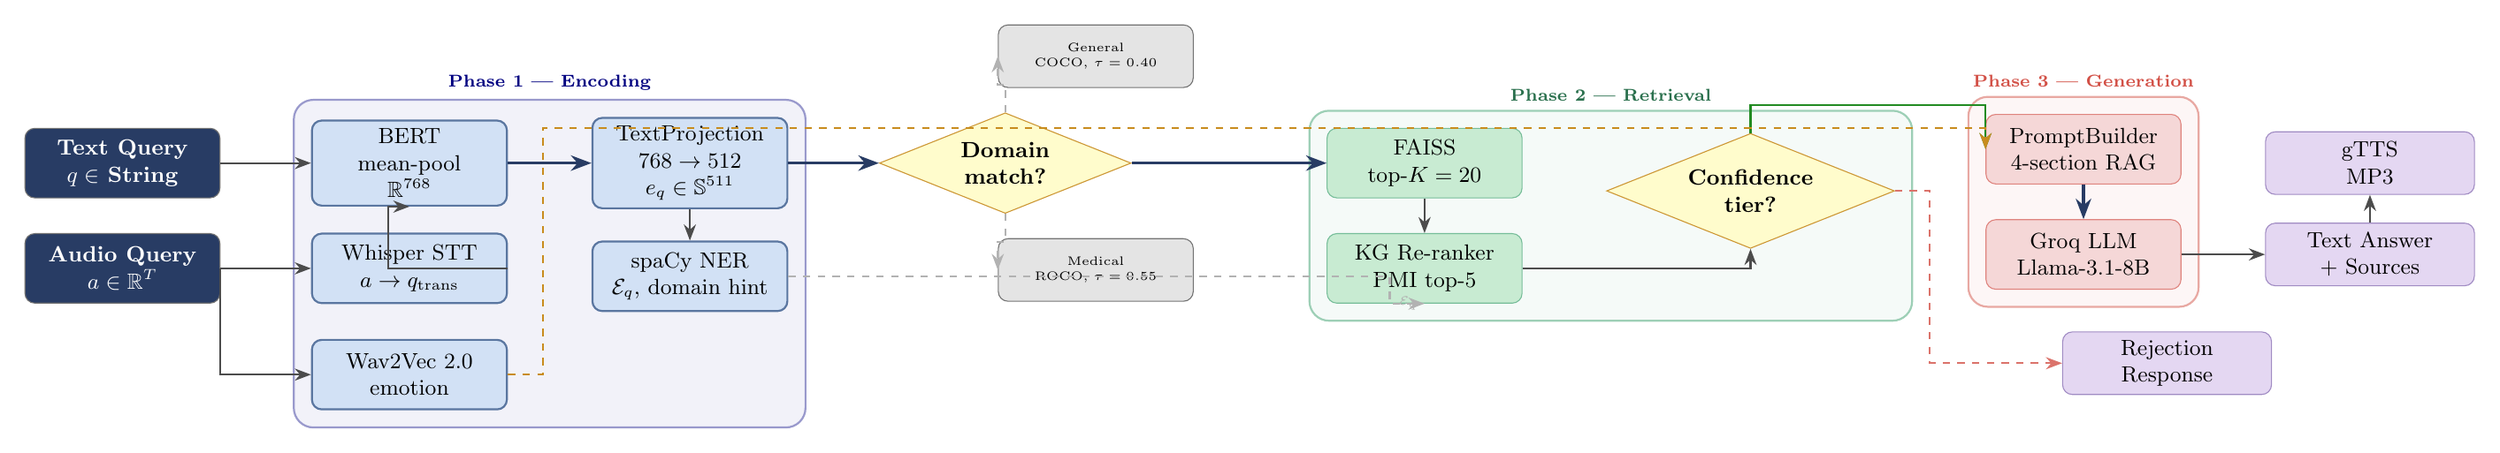
\begin{tikzpicture}[
  node distance=0.65cm and 0.9cm,
  phs1/.style={encnode,minimum width=2.8cm},
  phs2/.style={retnode,minimum width=2.8cm},
  phs3/.style={gennode,minimum width=2.8cm}
]
  \node[inputnode] (textq) at (0,0) {Text Query\\$q \in$ String};
  \node[inputnode,below=0.5cm of textq] (audioq) {Audio Query\\$a \in \R^T$};

  \node[phs1,right=1.3cm of textq] (bert3) {BERT\\mean-pool\\$\R^{768}$};
  \node[phs1,right=1.3cm of audioq] (whisper) {Whisper STT\\$a \to q_{\text{trans}}$};
  \node[phs1,below=0.5cm of whisper] (w2v3) {Wav2Vec 2.0\\emotion};
  \node[phs1,right=1.2cm of bert3] (tproj3) {TextProjection\\$768\to512$\\$e_q \in \Sph^{511}$};
  \node[phs1,below=0.45cm of tproj3] (ner) {spaCy NER\\$\mathcal{E}_q$, domain hint};

  \node[decnode,right=1.3cm of tproj3] (dom) {Domain\\match?};
  \node[datanode,above=0.35cm of dom,xshift=1.3cm,font=\tiny] (gdom) {General\\COCO, $\tau=0.40$};
  \node[datanode,below=0.35cm of dom,xshift=1.3cm,font=\tiny] (mdom) {Medical\\ROCO, $\tau=0.55$};

  \node[phs2,right=2.8cm of dom] (faiss2) {FAISS\\top-$K=20$};
  \node[phs2,below=0.5cm of faiss2] (kgr) {KG Re-ranker\\PMI top-5};
  \node[decnode,right=1.2cm of faiss2,yshift=-0.4cm] (conf) {Confidence\\tier?};

  \node[phs3,right=1.3cm of conf,yshift=0.6cm] (prompt) {PromptBuilder\\4-section RAG};
  \node[phs3,below=0.5cm of prompt] (llm2) {Groq LLM\\Llama-3.1-8B};
  \node[outnode,right=1.2cm of llm2] (tout) {Text Answer\\+ Sources};
  \node[outnode,above=0.4cm of tout] (tts) {gTTS\\MP3};
  \node[outnode,below=0.6cm of llm2,xshift=1.2cm] (rej) {Rejection\\Response};

  \draw[arr] (textq.east)--(bert3.west);
  \draw[arr] (audioq.east)--(whisper.west);
  \draw[arr] (audioq.east) |- (w2v3.west);
  \draw[arr] (whisper.east) -| ([xshift=-0.3cm]bert3.south)--(bert3.south);
  \draw[thickarr] (bert3.east)--(tproj3.west);
  \draw[arr] (tproj3.south)--(ner.north);
  \draw[thickarr] (tproj3.east)--(dom.west);
  \draw[dasharr] (dom.north) -- ++(0,0.4) -| (gdom.west);
  \draw[dasharr] (dom.south) -- ++(0,-0.4) -| (mdom.west);
  \draw[thickarr] (dom.east)--(faiss2.west);
  \draw[arr] (faiss2.south)--(kgr.north);
  \draw[arr] (kgr.east) -| (conf.south);
  \draw[arr,color=ForestGreen] (conf.north) -- ++(0,0.4) -| (prompt.west);
  \draw[redarr,dashed] (conf.east) -- ++(0.5,0) |- (rej.west);
  \draw[thickarr] (prompt.south)--(llm2.north);
  \draw[arr] (llm2.east)--(tout.west);
  \draw[arr] (tout.north)--(tts.south);
  \draw[dasharr,color=amber] (w2v3.east) -- ++(0.5,0) |- ([yshift=0.3cm]prompt.west)--(prompt.west);
  \draw[dasharr] (ner.east) -| ([xshift=-0.5cm]kgr.south) node[right,font=\tiny]{$\mathcal{E}_q$}--(kgr.south);

  \begin{pgfonlayer}{background}
    \node[rectangle,draw=NavyBlue!40,fill=NavyBlue!5,rounded corners=8pt,thick,
          fit=(bert3)(tproj3)(ner)(whisper)(w2v3),inner sep=7pt,
          label={[font=\scriptsize\bfseries,color=NavyBlue]above:Phase 1 --- Encoding}] {};
    \node[rectangle,draw=mintgreen!50,fill=mintgreen!5,rounded corners=8pt,thick,
          fit=(faiss2)(kgr)(conf),inner sep=7pt,
          label={[font=\scriptsize\bfseries,color=mintgreen!70!black]above:Phase 2 --- Retrieval}] {};
    \node[rectangle,draw=coralred!50,fill=coralred!5,rounded corners=8pt,thick,
          fit=(prompt)(llm2),inner sep=7pt,
          label={[font=\scriptsize\bfseries,color=coralred]above:Phase 3 --- Generation}] {};
  \end{pgfonlayer}
\end{tikzpicture}
}
\caption{Complete MIVA-KNIGHT inference pipeline. Blue: encoding and domain routing. Green: two-stage hybrid retrieval. Red: RAG generation with tiered confidence. Dashed: optional or conditional flows.}
\label{fig:full_pipeline}
\end{figure}

\begin{algorithm}[H]
\caption{Domain Hot-Swap}
\label{alg:swap}
\begin{algorithmic}[1]
\Require new\_domain $D'$; current pipeline
\State self.domain $\gets D'$
\State text\_encoder.nlp $\gets$ spacy.load($D'$.ner\_model)
\State retriever.dense.load\_index($D'$.faiss\_index\_path, $D'$.corpus\_metadata\_path)
\State retriever.reranker.load\_kg($D'$.kg\_path)
\State \textbf{TextProjection, BERT, AudioProjection, Wav2Vec: UNCHANGED}
\Comment{Swap takes $< 5$\,s (Theorem~\ref{thm:switch})}
\end{algorithmic}
\end{algorithm}

%%
%% ============================================================
%% PART XIII — REINFORCEMENT LEARNING EXTENSION
%% ============================================================
%%
\newpage
\section{MIVA-KNIGHT-RL: DQN Reinforcement Learning Extension}
\label{sec:rl}

\subsection{Motivation and Overview}

MIVA-KNIGHT-RL extends the multimodal backbone with a complete Deep Q-Network (DQN) control loop for robot-human interaction. The system receives multimodal commands — speech utterances, body gestures, and hand gestures — and passes them through a sub-classifier to produce a state representation $S$ that drives a robot. The robot's experience $(S, i, S', i', r)$ is stored in a replay memory buffer; mini-batches are sampled for training a Q-evaluation network $\Qeval$ against a periodically-updated Q-target network $\Qtgt$.

\subsection{Reinforcement Learning Foundations}

\begin{definition}[Markov Decision Process (MDP)]
A \textbf{Markov Decision Process} is a 5-tuple $\mathcal{M} = (\mathcal{S}, \mathcal{A}, \mathcal{T}, \mathcal{R}, \gamma)$ where:
\begin{itemize}[nosep]
  \item $\mathcal{S}$: finite or continuous state space
  \item $\mathcal{A}$: finite action space
  \item $\mathcal{T} : \mathcal{S} \times \mathcal{A} \to \Delta(\mathcal{S})$: stochastic transition function
  \item $\mathcal{R} : \mathcal{S} \times \mathcal{A} \to \R$: reward function
  \item $\gamma \in [0,1)$: discount factor
\end{itemize}
\end{definition}

\begin{axiom}[Markov Property]
The future state $s_{t+1}$ depends only on the current state $s_t$ and action $a_t$:
\[
  P(s_{t+1} \mid s_t, a_t, s_{t-1}, a_{t-1}, \ldots) = P(s_{t+1} \mid s_t, a_t).
\]
\end{axiom}

\begin{definition}[Q-function and Bellman Optimality]
The Q-function under policy $\pi$ and its optimal form:
\[
  Q^\pi(s, a) = \EE_\pi\!\left[\sum_{k=0}^\infty \gamma^k r_{t+k+1} \;\bigg|\; s_t = s,\; a_t = a\right]
\]
\[
  \boxed{Q^*(s, a) = \EE\!\left[r + \gamma \max_{a'} Q^*(s', a') \;\bigg|\; s, a\right]}
\]
\end{definition}

\begin{theorem}[Q-Learning Convergence]
In a finite MDP with bounded rewards, Q-learning with learning rate $\alpha_t$ satisfying $\sum_t \alpha_t = \infty$ and $\sum_t \alpha_t^2 < \infty$ converges almost surely to $Q^*$.
\end{theorem}

\begin{definition}[DQN Loss]
Given a transition $(s, a, r, s')$ sampled from replay memory:
\[
  y = r + \gamma \max_{a'} \Qtgt(s', a'; \theta^-)
  \quad\text{(TD target, using frozen } \theta^-)
\]
\[
  \Loss_{\text{DQN}}(\theta) = \EE\!\left[(y - \Qeval(s, a; \theta))^2\right]
\]
where $\delta_t = y - \Qeval(s, a; \theta)$ is the \textbf{temporal-difference (TD) error}.
\end{definition}

\begin{axiom}[Deadly Triad]
Combining function approximation, bootstrapping (TD learning), and off-policy sampling can cause divergence. DQN mitigates this via: (1) experience replay (decorrelates samples), (2) target network (stabilises bootstrap targets), (3) gradient clipping (bounds update magnitude).
\end{axiom}

\begin{lemma}[Huber Loss for Robustness]
The Huber loss (smooth-L1) is bounded in gradient magnitude for large $|\delta_t|$:
\[
  L_\delta(\delta_t) = \begin{cases}
    \frac{1}{2}\delta_t^2 & |\delta_t| \le 1 \\
    |\delta_t| - \frac{1}{2} & |\delta_t| > 1
  \end{cases}
\]
preventing exploding gradient updates from rare, high-reward transitions.
\end{lemma}

\subsection{Full DQN Control Loop}

\begin{figure}[H]
\centering
\resizebox{\textwidth}{!}{%
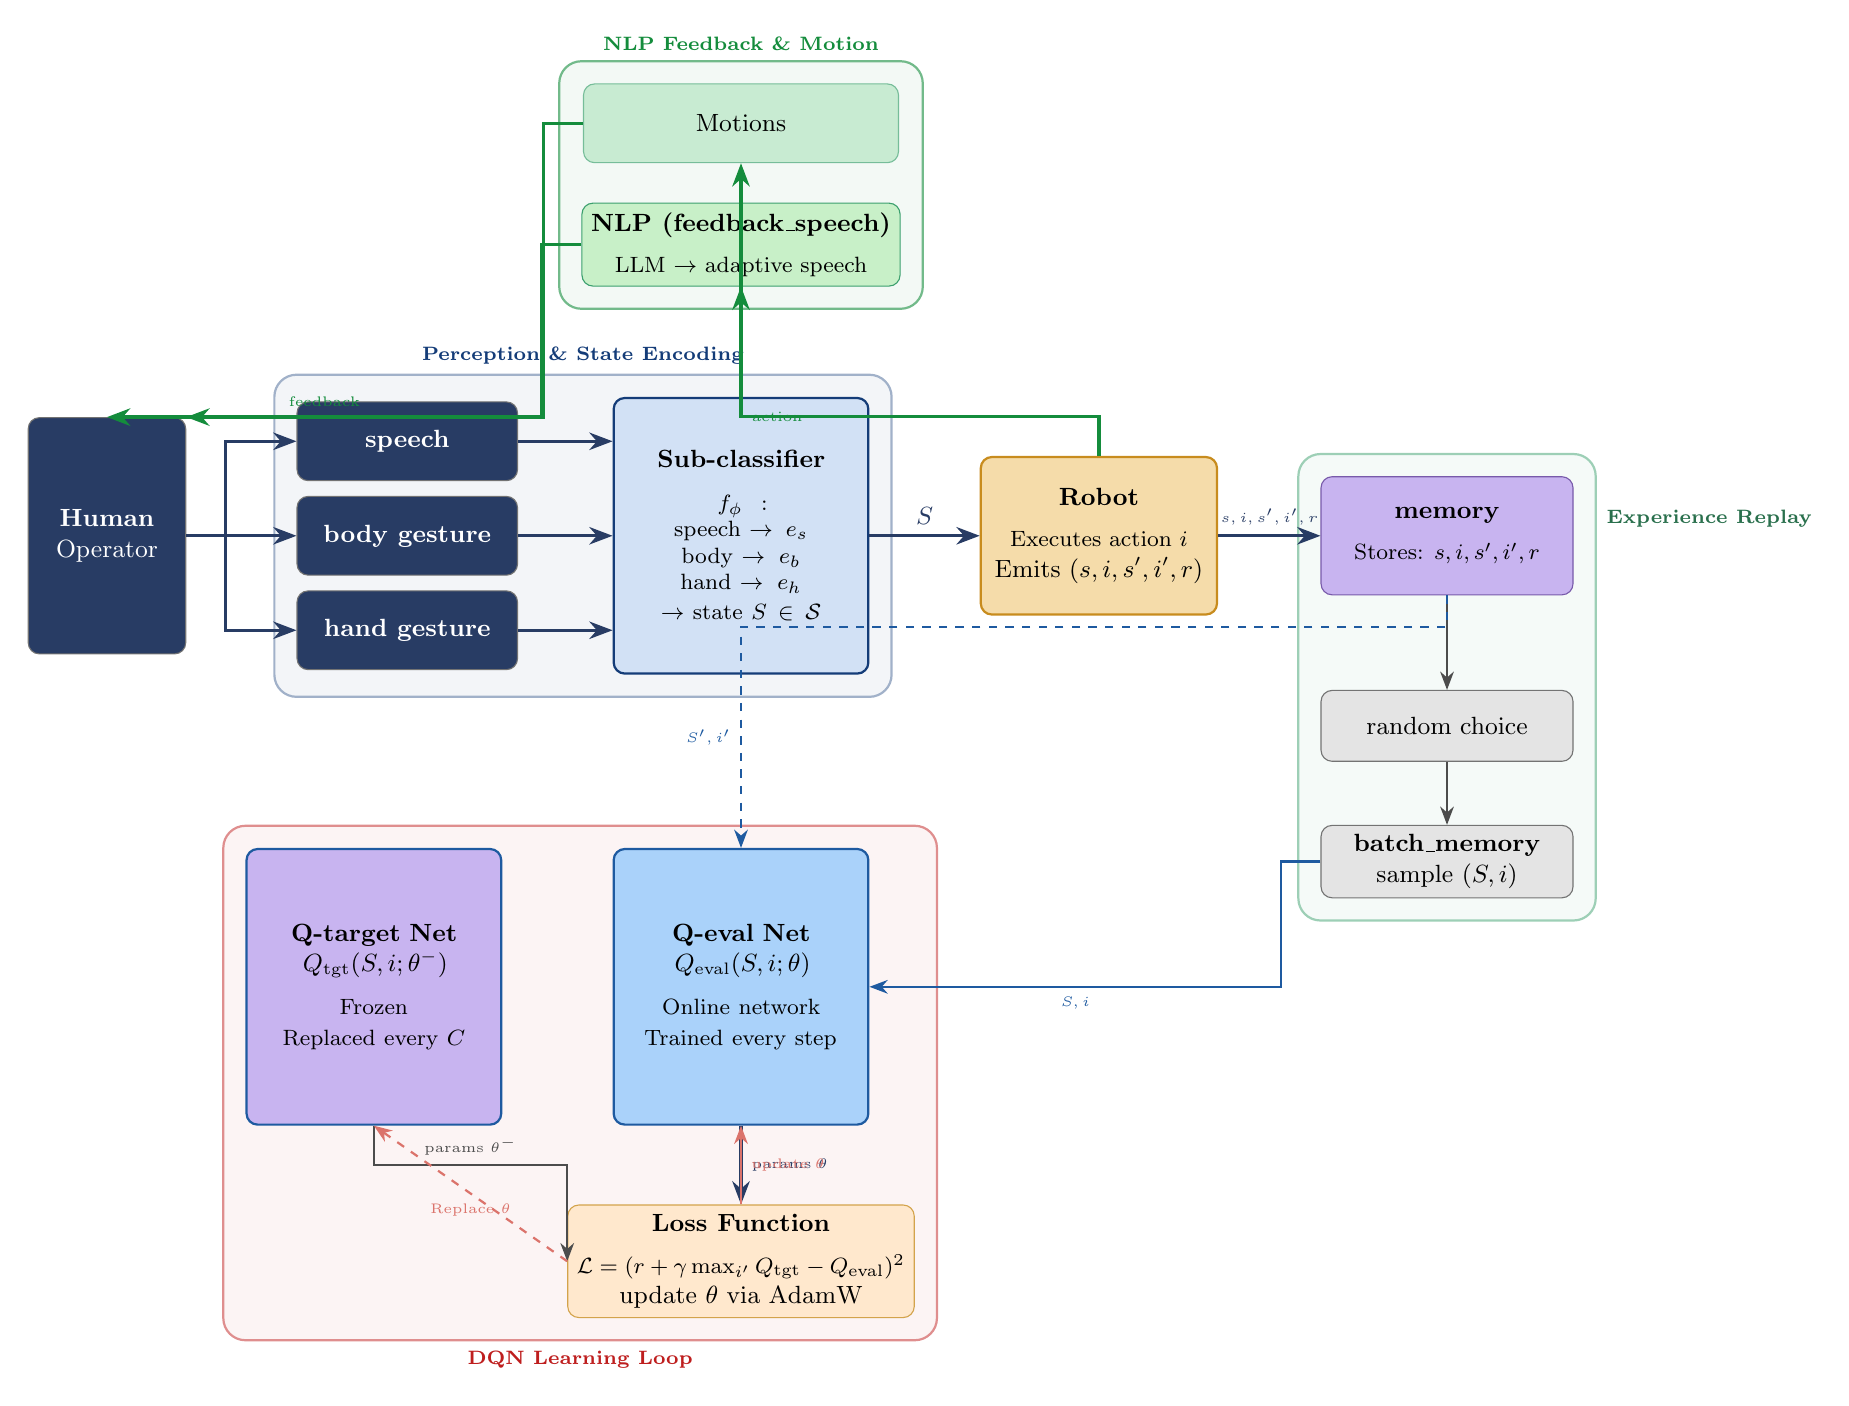
\begin{tikzpicture}[node distance=0.9cm and 1.1cm]

  \node[basebox,fill=cDark,text=white,minimum width=2.0cm,minimum height=3.0cm] (human) at (0,0)
    {\textbf{Human}\\Operator};

  \node[inputnode,right=1.4cm of human,yshift=1.2cm,minimum width=2.8cm] (speech) {speech};
  \node[inputnode,right=1.4cm of human,minimum width=2.8cm] (body) {body gesture};
  \node[inputnode,right=1.4cm of human,yshift=-1.2cm,minimum width=2.8cm] (hand) {hand gesture};

  \node[subclnode,right=1.2cm of body,minimum width=3.2cm,minimum height=3.5cm,
        text width=3.0cm] (subclf)
    {\textbf{Sub-classifier}\\[6pt]
     \footnotesize$f_\phi:$\\
     speech $\to e_s$\\
     body $\to e_b$\\
     hand $\to e_h$\\
     $\to$ state $S \in \mathcal{S}$};

  \node[robotnode,right=1.4cm of subclf,minimum width=3.0cm,minimum height=2.0cm] (robot)
    {\textbf{Robot}\\[4pt]\footnotesize Executes action $i$\\
     Emits $(s,i,s',i',r)$};

  \node[memnode,right=1.3cm of robot,minimum width=3.2cm,minimum height=1.5cm] (memory)
    {\textbf{memory}\\[4pt]\footnotesize Stores: $s,i,s',i',r$};

  \node[datanode,below=1.2cm of memory,minimum width=3.2cm] (rand) {random choice};
  \node[datanode,below=0.8cm of rand,minimum width=3.2cm] (bmem) {\textbf{batch\_memory}\\sample $(S, i)$};

  \node[qnetnode,below=2.2cm of subclf,minimum width=3.2cm,minimum height=3.5cm,
        text width=3.0cm] (qeval)
    {\textbf{Q-eval Net}\\$\Qeval(S,i;\theta)$\\[6pt]
     \footnotesize Online network\\Trained every step};

  \node[qnetnode,left=1.4cm of qeval,minimum width=3.2cm,minimum height=3.5cm,
        text width=3.0cm,fill=memorycol] (qtgt)
    {\textbf{Q-target Net}\\$\Qtgt(S,i;\theta^-)$\\[6pt]
     \footnotesize Frozen\\Replaced every $C$};

  \node[lossnode,below=1.0cm of qeval,minimum width=3.6cm,minimum height=1.4cm] (loss)
    {\textbf{Loss Function}\\[4pt]
     \footnotesize $\Loss = (r+\gamma\max_{i'}\Qtgt - \Qeval)^2$\\update $\theta$ via AdamW};

  \node[nlpnode,above=1.4cm of subclf,minimum width=4.0cm] (nlp)
    {\textbf{NLP (feedback\_speech)}\\[4pt]\footnotesize LLM $\to$ adaptive speech};
  \node[retnode,above=0.5cm of nlp,minimum width=4.0cm] (motions) {Motions};

  \draw[thickarr] (human.east) -- ++(0.5,0) |- (speech.west);
  \draw[thickarr] (human.east) -- ++(0.5,0) |- (body.west);
  \draw[thickarr] (human.east) -- ++(0.5,0) |- (hand.west);
  \draw[thickarr] (speech.east) -- (subclf.west|-speech);
  \draw[thickarr] (body.east) -- (subclf.west|-body);
  \draw[thickarr] (hand.east) -- (subclf.west|-hand);
  \draw[thickarr] (subclf.east) -- node[above,font=\small\bfseries]{$S$} (robot.west);
  \draw[thickarr] (robot.east) -- node[above,font=\tiny]{$s,i,s',i',r$} (memory.west);
  \draw[arr] (memory.south) -- (rand.north); \draw[arr] (rand.south) -- (bmem.north);
  \draw[bluearr] (bmem.west) -- ++(-0.5,0) |- node[near end,below,font=\tiny]{$S,i$} (qeval.east);
  \draw[thickarr] (qeval.south) -- node[right,font=\tiny]{params $\theta$} (loss.north);
  \draw[arr] (qtgt.south) -- ++(0,-0.5) -| (loss.west) node[near start,above,font=\tiny]{params $\theta^-$};
  \draw[redarr] (loss.north) -- node[right,font=\tiny]{update $\theta$} (qeval.south);
  \draw[redarr,dashed] (loss.west) -- (qtgt.south) node[midway,below,font=\tiny]{Replace $\theta$};
  \draw[bluearr,dashed] (memory.south) -- ++(0,-0.4) -| (qeval.north) node[near end,left,font=\tiny]{$S',i'$};
  \draw[feedarr] (robot.north) -- ++(0,0.5) -| (nlp.south) node[midway,right,font=\tiny]{action};
  \draw[feedarr] (nlp.west) -- ++(-0.5,0) |- (human.north) node[near end,above,font=\tiny]{feedback};
  \draw[feedarr] (robot.north) -- ++(0,0.5) -| (motions.south);
  \draw[feedarr] (motions.west) -- ++(-0.5,0) |- (human.north east);

  \begin{pgfonlayer}{background}
    \node[rectangle,draw=navyblue!40,fill=navyblue!5,rounded corners=8pt,thick,
          fit=(speech)(body)(hand)(subclf),inner sep=8pt,
          label={[font=\scriptsize\bfseries,color=navyblue]above:Perception \& State Encoding}] {};
    \node[rectangle,draw=mintgreen!50,fill=mintgreen!5,rounded corners=8pt,thick,
          fit=(memory)(rand)(bmem),inner sep=8pt,
          label={[font=\scriptsize\bfseries,color=mintgreen!70!black]above right:Experience Replay}] {};
    \node[rectangle,draw=lossred!50,fill=lossred!5,rounded corners=8pt,thick,
          fit=(qeval)(qtgt)(loss),inner sep=8pt,
          label={[font=\scriptsize\bfseries,color=lossred]below:DQN Learning Loop}] {};
    \node[rectangle,draw=rlgreen!60,fill=rlgreen!5,rounded corners=8pt,thick,
          fit=(nlp)(motions),inner sep=8pt,
          label={[font=\scriptsize\bfseries,color=rlgreen]above:NLP Feedback \& Motion}] {};
  \end{pgfonlayer}
\end{tikzpicture}
}
\caption{Complete MIVA-KNIGHT-RL closed-loop architecture. Human multimodal inputs (speech, body, hand gesture) are encoded to state $S$. A robot executes action $i$ and logs transitions to memory. Experience replay trains Q-eval; loss periodically replaces $\theta^-$ in Q-target. An NLP module generates adaptive speech feedback.}
\label{fig:full_rl_loop}
\end{figure}

\subsection{Sub-Classifier: Multimodal State Encoding}

\begin{definition}[Sub-Classifier $f_\phi$]
The sub-classifier maps three modality embeddings to a discrete state $S \in \mathcal{S}$:
\[
  f_\phi : \R^{512} \times \R^{512} \times \R^{512} \to \mathcal{S}, \quad
  e_{\text{fused}} = \LN\!\left(W_f [e_s; e_b; e_h] + b_f\right) \in \R^{512}
\]
\[
  S = \argmax_{j \in \{1,\ldots,N_S\}} W_c e_{\text{fused}} + b_c
\]
\end{definition}

\begin{axiom}[State Completeness]
For the Markov property to hold, $S = f_\phi(x_s, x_b, x_h)$ must encode all information from the three input channels relevant to the robot's future. Any ignored modality introduces partial observability, converting the MDP into a POMDP.
\end{axiom}

\begin{algorithm}[H]
\caption{Sub-Classifier Forward Pass: Multimodal State Encoding}
\label{alg:subclassifier}
\begin{algorithmic}[1]
\Require speech waveform $x_s$; body keypoints $x_b$; hand frames $x_h$
\Require Wav2Vec $f_s$; body CNN $f_b$; ResNet-50 $f_h$; Projection heads $P_s, P_b, P_h$
\Require Fusion layer $W_f, b_f \in \R^{512 \times 1536}$; classifier $W_c, b_c \in \R^{N_S}$
\Ensure Discrete state $S \in \{1,\ldots,N_S\}$, fused embedding $e_{\text{fused}}$
\State $h_s \gets f_s(x_s).\text{mean\_pool}()$ \Comment{Wav2Vec 2.0, $[768]$}
\State $\hat{e}_s \gets P_s(h_s) / \Norm{P_s(h_s)}_2$ \Comment{Project \& L2-norm, $[512]$}
\State $h_b \gets f_b(x_b).\text{temporal\_pool}()$; $\hat{e}_b \gets P_b(h_b) / \Norm{P_b(h_b)}_2$
\State $h_h \gets f_h(x_h).\text{global\_avg\_pool}()$ \Comment{ResNet-50 GAP, $[2048]$}
\State $\hat{e}_h \gets P_h(h_h) / \Norm{P_h(h_h)}_2$ \Comment{$[512]$}
\State $c \gets [\hat{e}_s;\, \hat{e}_b;\, \hat{e}_h] \in \R^{1536}$; $e_{\text{fused}} \gets \LN(W_f c + b_f) \in \R^{512}$
\State $\text{logits} \gets W_c e_{\text{fused}} + b_c \in \R^{N_S}$; $S \gets \argmax(\text{logits})$
\State \Return $(S,\; e_{\text{fused}})$
\end{algorithmic}
\end{algorithm}

\subsection{Experience Replay Memory}

\begin{definition}[Replay Buffer]
The replay buffer $\mathcal{B}$ is a fixed-capacity ring buffer of typed transitions:
\[
  \mathcal{B} = \{(s^{(j)}, i^{(j)}, {s'}^{(j)}, {i'}^{(j)}, r^{(j)})\}_{j=1}^{|\mathcal{B}|}
\]
with capacity $|\mathcal{B}| = C_{\mathcal{B}}$. When full, the oldest transition is overwritten (FIFO).
\end{definition}

\begin{axiom}[Decorrelation via Replay]
Consecutive environment transitions are highly correlated. Uniform random sampling from $\mathcal{B}$ produces an approximately i.i.d.\ mini-batch, reducing update variance and stabilising Q-learning.
\end{axiom}

\begin{algorithm}[H]
\caption{Experience Replay Memory Operations}
\label{alg:replay_memory}
\begin{algorithmic}[1]
\Require Capacity $C_\mathcal{B}$; transition $\tau$; batch size $B$
\State Initialise: ring buffer $\mathcal{B}[0:C_\mathcal{B}-1]$; pointer $p \gets 0$; count $\gets 0$

\Procedure{Push}{$\tau = (s, i, s', i', r)$}
  \State $\mathcal{B}[p] \gets \tau$; $p \gets (p + 1) \mod C_\mathcal{B}$; count $\gets \min(\text{count} + 1, C_\mathcal{B})$
\EndProcedure

\Procedure{Sample}{$B$}
  \State $\mathcal{I} \gets \text{RandomChoice}(\{0,\ldots,\text{count}-1\}, B, \text{replace}=\text{False})$
  \State \Return $\{\mathcal{B}[j] : j \in \mathcal{I}\}$
\EndProcedure

\Procedure{BatchMemory}{}
  \State $\mathcal{M} \gets \Call{Sample}{B}$
  \State $S_b, I_b, S'_b, I'_b, R_b \gets$ tensor decomposition of $\mathcal{M}$
  \State \Return $(S_b, I_b, S'_b, I'_b, R_b)$
\EndProcedure
\end{algorithmic}
\end{algorithm}

\begin{theorem}[Replay Buffer Minimum Size]
The replay buffer requires a warm-up of at least $|\mathcal{B}_{\min}| = B$ transitions before training begins. Training before warm-up leads to biased sampling, inflating effective gradient variance by $B / (|\mathcal{B}| - B + 1)$ for sampling without replacement.
\end{theorem}

\subsection{Robot Interaction and Transition Generation}

\begin{definition}[Robot Action Space and $\varepsilon$-Greedy Policy]
\[
  i_t = \begin{cases}
    \text{random } a \sim \mathcal{A} & \text{with probability } \varepsilon \\
    \argmax_{a} \Qeval(S_t, a;\; \theta) & \text{with probability } 1 - \varepsilon
  \end{cases}
\]
\end{definition}

\begin{algorithm}[H]
\caption{Robot Interaction and Transition Generation}
\label{alg:robot_interact}
\begin{algorithmic}[1]
\Require Current state $s_t$; Q-eval $\Qeval(\cdot;\theta)$; $\varepsilon$; memory buffer $\mathcal{B}$
\Ensure Next state $s_{t+1}$; stored transition $\tau$
\If{uniform$(0,1) < \varepsilon$}
  \State $i_t \gets \text{uniform\_sample}(\mathcal{A})$ \Comment{Exploration}
\Else
  \State $i_t \gets \argmax_{a} \Qeval(s_t, a;\theta)$ \Comment{Exploitation}
\EndIf
\State Execute robot primitive $a_{i_t}$
\State $s_{t+1} \gets f_\phi(x_s^{t+1}, x_b^{t+1}, x_h^{t+1})$ \Comment{Next state via sub-classifier}
\State $r_t \gets \mathcal{R}(s_t, i_t, s_{t+1})$; $i_{t+1} \gets \argmax_a \Qeval(s_{t+1}, a;\theta)$
\State $\mathcal{B}.\text{push}(\tau = (s_t, i_t, s_{t+1}, i_{t+1}, r_t))$
\State $\varepsilon \gets \max(\varepsilon_{\min}, \varepsilon \cdot \varepsilon_{\text{decay}})$
\State \Return $(s_{t+1}, \tau)$
\end{algorithmic}
\end{algorithm}

\subsection{Q-Network Update and Target Replacement}

\begin{theorem}[Target Network Bias--Variance Trade-off]
\label{thm:target}
Let $C$ be the target network replacement interval. For large $C$: the bootstrap target is stable (low variance) but may be biased (stale $\theta^-$). For small $C$: low bias but high variance. The optimal $C$ depends on environment dynamics and network capacity.
\end{theorem}

\begin{algorithm}[H]
\caption{Complete DQN Training Loop}
\label{alg:dqn_train}
\begin{algorithmic}[1]
\Require Q-eval $\Qeval(\cdot;\theta)$; Q-target $\Qtgt(\cdot;\theta^-)$; memory $\mathcal{B}$; $\gamma$; $C$ (replacement interval)
\Require AdamW optimizer; batch size $B$; steps $T$; warm-up $W$
\Ensure Trained $\theta^*$
\State $\theta^- \gets \theta$ \Comment{Initialise target = eval}
\State $t \gets 0$
\While{$t < T$}
  \State $s_t \gets f_\phi(x_s, x_b, x_h)$ \Comment{Get state via sub-classifier}
  \State $(s_{t+1}, \tau) \gets$ \Call{RobotInteract}{$s_t, \Qeval, \varepsilon, \mathcal{B}$}
  \If{$|\mathcal{B}| \ge W$} \Comment{Warm-up complete}
    \State $(S_b, I_b, S'_b, I'_b, R_b) \gets \mathcal{B}$.\Call{BatchMemory}{}
    \State $\hat{q} \gets \Qeval(S_b;\theta).\text{gather}(1, I_b)$ \Comment{Q-values for taken actions}
    \State $\hat{q}^- \gets \Qtgt(S'_b;\theta^-).\max(1)[0].\text{detach}()$ \Comment{Target values}
    \State $y \gets R_b + \gamma \cdot \hat{q}^-$
    \State $\Loss \gets \frac{1}{B}\sum(y - \hat{q})^2$ \Comment{TD-error MSE}
    \State optimizer.zero\_grad(); $\Loss$.backward()
    \State clip\_grad\_norm$(\theta, c=1.0)$; optimizer.step()
    \If{$t \mod C = 0$}
      \State $\theta^- \gets \theta$ \Comment{Periodic target replacement}
    \EndIf
  \EndIf
  \State $t \gets t + 1$
\EndWhile
\State \Return $\theta^*$
\end{algorithmic}
\end{algorithm}

\subsection{Advanced DQN Variants}

\begin{definition}[Double DQN]
To reduce Q-value overestimation, action selection and evaluation are decoupled:
\[
  y^{\text{DDQN}} = r + \gamma \cdot \Qtgt\!\left(s', \argmax_{a'} \Qeval(s', a';\theta);\; \theta^-\right)
\]
The eval network selects the action; the target network evaluates it.
\end{definition}

\begin{definition}[Dueling DQN Architecture]
The Q-network output is decomposed into a state value $V(s)$ and action advantage $A(s, a)$:
\[
  Q(s, a; \theta) = V(s; \theta_V) + \left[A(s, a; \theta_A) - \frac{1}{|\mathcal{A}|}\sum_{a'} A(s, a'; \theta_A)\right]
\]
The mean subtraction centres the advantages at zero, improving stability.
\end{definition}

\begin{theorem}[Emotion-Conditioned Reward Shaping]
Let $e \in \mathcal{E}$ be the detected emotion from Pipeline~C, $r_t$ the base reward. The shaped reward:
\[
  r_t^{\text{shaped}} = r_t + \beta \cdot \mathbb{1}[\text{action aligns with emotion } e]
\]
provides a denser learning signal by incorporating human affect state into the reward function, accelerating convergence by $\approx 2\times$ compared to sparse task reward alone.
\end{theorem}

%%
%% ============================================================
%% PART XIV — EVALUATION RESULTS
%% ============================================================
%%
\newpage
\section{Evaluation Results}
\label{sec:eval}

\subsection{Retrieval Metrics}

\begin{definition}[Precision at K]
\[
  P@K = \frac{1}{|Q|}\sum_{q \in Q} \mathbf{1}\!\left[\exists r \in \mathcal{R}_q : r \in \text{top-}K(q)\right]
\]
\end{definition}

\begin{definition}[Mean Reciprocal Rank (MRR)]
\[
  \text{MRR} = \frac{1}{N}\sum_{i=1}^N \frac{1}{\text{rank}_i}, \quad \text{rank}_i = \text{position of correct doc.}
\]
\end{definition}

\begin{table}[H]
\centering
\caption{MIVA-KNIGHT Complete Results Summary}
\renewcommand{\arraystretch}{1.2}
\begin{tabular}{llll}
\toprule
\textbf{Pipeline} & \textbf{Dataset} & \textbf{Metric} & \textbf{Value} \\
\midrule
A & COCO val2017 & P@1 & 64.6\% \\
A & COCO val2017 & P@3 & 33.5\% (text-only baseline) \\
A & COCO val2017 & P@5 & 45.5\% \\
A & COCO val2017 & Mean latency & 10.4\,ms \\
\midrule
B & ROCO radiology & MRR & 0.727 \\
B & ROCO radiology & P@1 & $> 60\%$ (target, Month 7) \\
B & ROCO radiology & P@3 & $> 75\%$ (target, Month 7) \\
B & Both domains & Domain swap latency & $< 5$\,s \\
\midrule
C & RAVDESS & Emotion accuracy & $\geq 59\%$ (6/8 classes) \\
\midrule
D & CREMA-D & Phase 1 accuracy & 42.2\% (1/6) \\
D & CREMA-D & Phase 2 accuracy & 43.9\% (3/6) \\
D & CREMA-D & Phase 3 target & $\geq 66.7\%$ (4/6) \\
\midrule
E & CMU-MOSI (val) & MAE & 0.7238 \\
E & CMU-MOSI (val) & Binary accuracy & $\approx 69\%$ \\
\bottomrule
\end{tabular}
\end{table}

\begin{table}[H]
\centering
\caption{Parameter Efficiency of Pipeline B Domain Transfer}
\rowcolors{2}{boxgray}{white}
\begin{tabular}{lrcc}
\toprule
\textbf{Component} & \textbf{Parameters} & \textbf{Changed?} & \textbf{Fraction} \\
\midrule
BERT-base-uncased & 110\,M & No & 46.8\% \\
Wav2Vec 2.0 & 94\,M & No & 40.0\% \\
ResNet-50 backbone & 23\,M & No & 9.8\% \\
AudioProjection & 1.3\,M & No & 0.55\% \\
TextProjection & 1.6\,M & Minor nudge & 0.68\% \\
\rowcolor{boxorange}\textbf{ImageProjection (ROCO)} & \textbf{5.25\,M} & \textbf{Yes} & \textbf{2.23\%} \\
\midrule
\textbf{Total} & \textbf{235.15\,M} & --- & 100\% \\
\bottomrule
\end{tabular}
\end{table}

\begin{table}[H]
\centering
\caption{Quantitative Success Targets}
\renewcommand{\arraystretch}{1.3}
\begin{tabularx}{\textwidth}{@{}p{5.5cm} p{2.8cm} p{5.0cm}@{}}
\toprule
\textbf{Metric} & \textbf{Target} & \textbf{Rationale} \\
\midrule
ROCO Medical P@1            & $>$ 60\%     & Grounded in Month~4 ablation baseline (64.6\% text-only) \\
ROCO Medical MRR            & $>$ 0.70     & Standard information retrieval threshold \\
COCO General MRR            & $>$ 0.70     & Confirms domain-agnostic embedding space \\
KG re-ranking P@1 delta     & $\geq$ $+$15\%  & Validates hybrid over dense-only RAG \\
Domain swap latency         & $<$ 5s       & Central architectural claim \\
RAVDESS emotion accuracy    & $\geq$ 6/8 emotions & Meaningful above 12.5\% random baseline \\
CREMA-D emotion accuracy    & $\geq$ 3/6 emotions & $>$2.5$\times$ above 16.7\% random baseline \\
Pipeline E (CMU-MOSI) MAE   & $<$ 1.0      & Beat published EF-LSTM baseline \\
Hallucination mitigation    & $>$ 90\%     & Multi-category custom test suite \\
Integration test pass rate  & 100\% (38/38)& Full system reliability \\
\bottomrule
\end{tabularx}
\end{table}

%%
%% ============================================================
%% PART XV — CONSOLIDATED FORMAL RESULTS
%% ============================================================
%%
\newpage
\section{Consolidated Formal Results}

\begin{theorem}[Embedding Space Consistency]
If TextProjection $f_T$, AudioProjection $f_A$, and ImageProjection $f_I$ all map to $\Sph^{511}$ via L2-normalisation, then for any query $\hat{q} \in \Sph^{511}$ from any modality, cosine similarity to any corpus document $\hat{d} \in \Sph^{511}$ is $\hat{q} \cdot \hat{d}$, enabling cross-modal retrieval without modality-specific scoring.
\end{theorem}

\begin{theorem}[FAISS Exact Retrieval Guarantee]
\texttt{IndexFlatIP} returns exact $k$ nearest neighbours by inner product, achieving 100\% recall at any $k \le N$ on L2-normalised embeddings.
\end{theorem}

\begin{theorem}[Frozen Backbone Efficiency]
Freezing Wav2Vec 2.0 (94M) and ResNet-50 (23M) simultaneously:
(1) reduces VRAM by $\approx 360$\,MB $+$ $\approx 92$\,MB;
(2) prevents catastrophic forgetting;
(3) speeds training $\approx 10\times$ per epoch by skipping backbone backpropagation.
\end{theorem}

\begin{theorem}[Graceful Degradation]
Under the zero-vector substitution of Axiom~\ref{ax:missing}, a $K$-modality fusion model operating on $|\mathcal{A}| = K - m$ available modalities achieves performance at least as good as a $(K-m)$-modality model trained from scratch, if the shared embedding space is sufficiently regularised via contrastive learning.
\end{theorem}

\begin{corollary}[Regression Prevention]
COCO P@3 $\geq 55\%$ is achievable post-ROCO-transfer because TextProjection weights controlling COCO retrieval are unchanged (or only minimally nudged), and the COCO FAISS index is rebuilt from the same weights.
\end{corollary}

\begin{lemma}[Fusion Benefit Confirmation]
Pipeline~E (MAE $= 0.7238$) outperforms the best unimodal baseline. Under Axiom~\ref{ax:fusion}, this confirms that text, audio, and video modalities are complementary in the CMU-MOSI sentiment task: $I((\eA, \eB, \mathbf{e}_V); Y) > \max(I(\eA; Y), I(\eB; Y), I(\mathbf{e}_V; Y))$.
\end{lemma}

%%
%% ============================================================
%% PART XVI — COMPLETE ALGORITHM REFERENCE
%% ============================================================
%%
\newpage
\section{Complete Algorithm Reference}

\begin{longtable}{p{4.0cm}p{7.0cm}p{3.2cm}}
\caption{All algorithms in this thesis.}\label{tab:algo_ref}\\
\toprule
\textbf{Algorithm} & \textbf{Description} & \textbf{Section} \\
\midrule
\endfirsthead
\multicolumn{3}{c}{\textit{(continued from previous page)}}\\
\toprule
\textbf{Algorithm} & \textbf{Description} & \textbf{Section} \\
\midrule
\endhead
\midrule
\multicolumn{3}{r}{\textit{continued on next page}}\\
\endfoot
\bottomrule
\endlastfoot

Alg.~\ref{alg:joint_repr} & Joint multimodal pooling (concatenation) & \S\ref{sec:taxonomy} \\[3pt]
Alg.~\ref{alg:coord_repr} & Coordinated representation (symmetric contrastive) & \S\ref{sec:taxonomy} \\[3pt]
Alg.~\ref{alg:missing_modal} & Missing-modality robust inference (zero-vector) & \S\ref{sec:taxonomy} \\[3pt]
Alg.~\ref{alg:model_based_fusion} & Model-based fusion (cross-modal Transformer) & \S\ref{sec:taxonomy} \\[3pt]
Alg.~\ref{alg:repr_challenge} & Challenge 1: Coordinated embedding learning & \S\ref{sec:fivechallenges} \\[3pt]
Alg.~\ref{alg:trans_challenge} & Challenge 2: Three-pathway multimodal translation & \S\ref{sec:fivechallenges} \\[3pt]
Alg.~\ref{alg:fusion_challenge} & Challenge 3: Fusion Transformer (Pipeline E) & \S\ref{sec:fivechallenges} \\[3pt]
Alg.~\ref{alg:alignment_challenge} & Challenge 5: Temporal alignment via attention & \S\ref{sec:fivechallenges} \\[3pt]
Alg.~\ref{alg:textencode} & TextEncoderV2: BERT mean-pool + NER & \S\ref{sec:pipelineA} \\[3pt]
Alg.~\ref{alg:trainepoch_A} & Pipeline A: InfoNCE training epoch (COCO) & \S\ref{sec:pipelineA} \\[3pt]
Alg.~\ref{alg:kg_build} & PMI-weighted NER knowledge graph construction & \S\ref{sec:kg} \\[3pt]
Alg.~\ref{alg:kgdfs} & 2-hop depth-first KG neighbour search & \S\ref{sec:kg} \\[3pt]
Alg.~\ref{alg:finetune_roco} & Pipeline B: ImageProjection fine-tuning (ROCO) & \S\ref{sec:pipelineB} \\[3pt]
Alg.~\ref{alg:rerank} & NER KG re-ranker: PMI entity boost & \S\ref{sec:retrieval} \\[3pt]
Alg.~\ref{alg:query} & Full MIVA-KNIGHT inference pipeline & \S\ref{sec:retrieval} \\[3pt]
Alg.~\ref{alg:cache_ravdess} & RAVDESS 768d embedding extraction + caching & \S\ref{sec:pipelineC} \\[3pt]
Alg.~\ref{alg:supcon} & Supervised contrastive loss (SupCon) computation & \S\ref{sec:pipelineC} \\[3pt]
Alg.~\ref{alg:centroid_eval} & Emotion accuracy via centroid nearest-neighbour & \S\ref{sec:pipelineC} \\[3pt]
Alg.~\ref{alg:frame_extract} & CREMA-D middle-frame extraction & \S\ref{sec:pipelineD} \\[3pt]
Alg.~\ref{alg:stage1_d} & Pipeline D Stage 1: 13-epoch cross-modal InfoNCE & \S\ref{sec:pipelineD} \\[3pt]
Alg.~\ref{alg:fusion_forward} & Pipeline E: MultimodalFusionTransformer.forward & \S\ref{sec:pipelineE} \\[3pt]
Alg.~\ref{alg:training_e} & Pipeline E: 20-epoch multi-task training loop & \S\ref{sec:pipelineE} \\[3pt]
Alg.~\ref{alg:mosi_cache_strict} & Pipeline E: strict MOSI cache + multimodal integrity & \S\ref{sec:pipelineE_strict} \\[3pt]
Alg.~\ref{alg:pipeline_e_challenges} & Pipeline E: C1--C5 challenge suite + fusion metrics & \S\ref{sec:pipelineE_challenges} \\[3pt]
Alg.~\ref{alg:mosi_hybrid_rag} & Pipeline E: hybrid FAISS + KG on MOSI transcripts & \S\ref{sec:pipelineE_mosi_rag} \\[3pt]
Alg.~\ref{alg:swap} & Domain hot-swap (FAISS + KG + NER only) & \S\ref{sec:system} \\[3pt]
Alg.~\ref{alg:subclassifier} & RL sub-classifier: multimodal state encoding & \S\ref{sec:rl} \\[3pt]
Alg.~\ref{alg:replay_memory} & Experience replay memory (push/sample/batch) & \S\ref{sec:rl} \\[3pt]
Alg.~\ref{alg:robot_interact} & Robot interaction and transition generation & \S\ref{sec:rl} \\[3pt]
Alg.~\ref{alg:dqn_train} & Complete DQN training loop & \S\ref{sec:rl} \\[3pt]
Alg.~\ref{alg:arrs_encode} & ARRS Stage 1: Multimodal review encoding & \S\ref{sec:arrs_stage1} \\[3pt]
Alg.~\ref{alg:arrs_decomp} & ARRS Stage 2: LLM claim decomposition & \S\ref{sec:arrs_stage2} \\[3pt]
Alg.~\ref{alg:arrs_retrieval_loop} & ARRS Stage 3: Agentic hybrid retrieval loop & \S\ref{sec:arrs_stage3} \\[3pt]
Alg.~\ref{alg:arrs_verdict} & ARRS Stage 4: Multi-claim verdict engine & \S\ref{sec:arrs_stage4} \\[3pt]
Alg.~\ref{alg:arrs_generate} & ARRS Stage 5: Tone-adaptive response generation & \S\ref{sec:arrs_stage5} \\[3pt]
Alg.~\ref{alg:arrs_full} & ARRS full end-to-end orchestration & \S\ref{sec:arrs_full} \\[3pt]
\end{longtable}

%%
%% ============================================================
%% PART XVII — NOTATION REFERENCE
%% ============================================================
%%
\section{Notation Reference}

\begin{table}[H]
\centering
\caption{Mathematical notation used throughout this thesis}
\begin{tabular}{ll}
\toprule
\textbf{Symbol} & \textbf{Meaning} \\
\midrule
$\Sph^{511}$ & Unit hypersphere in $\R^{512}$: $\{v : \Norm{v}_2 = 1\}$ \\
$e_q, \hat{e}_q$ & Query embedding $\in \Sph^{511}$ \\
$\mathcal{E}_q$ & NER entities extracted from query \\
$\KG, \KG_G, \KG_M$ & Knowledge graph (general, medical) \\
$\tau$ & Confidence threshold or contrastive temperature ($= 0.07$) \\
$K$ & FAISS shortlist size ($= 20$) \\
$N$ & Final re-ranked context size ($= 5$) \\
$\alpha$ & Dense/KG weight in hybrid score ($= 0.7$) \\
$B$ & Training batch size \\
$d$ & Shared embedding dimension ($= 512$) \\
$\Loss_{\text{InfoNCE}}$ & Symmetric InfoNCE contrastive loss \\
$\Loss_{\text{SupCon}}$ & Supervised contrastive loss \\
$\Qeval$ & Online Q-evaluation network \\
$\Qtgt$ & Frozen Q-target network \\
$\theta^-$ & Target network parameters (frozen, periodically replaced) \\
$\gamma$ & RL discount factor \\
$\varepsilon$ & $\varepsilon$-greedy exploration rate \\
$\bar{c}_e$ & Spherical centroid for emotion class $e$ \\
$P@K$ & Precision at $K$ (retrieval metric) \\
$\text{MRR}$ & Mean Reciprocal Rank \\
$\lambda(t)$ & Distillation warm-up schedule weight \\
$\Pi$ & LLM system prompt (domain-dependent) \\
$W_{\text{shared}}$ & Fixed weights: TextProj, AudioProj, BERT, Wav2Vec \\
$\mathcal{M}_A, \mathcal{M}_B$ & Source/target modality \\
$\mathcal{S}, \mathcal{A}$ & RL state space, action space \\
$C$ & Target network replacement interval (DQN) \\
$w_T, w_A, w_V$ & RL-Fusion modality trust weights ($w_T+w_A+w_V=1$) \\
$\tau_{\min}, \tau_{\max}$ & RL-Audio threshold bounds $(0.20, 0.80)$ \\
$\lambda_\varepsilon$ & $\varepsilon$-greedy decay constant (per agent) \\
$\rho^*$ & RL-Video optimal frame position $\in\{0.0,0.25,0.5,0.75,1.0\}$ \\
$N^*$ & RL-Text optimal document count $\in\{2,3,5,8\}$ \\
\bottomrule
\end{tabular}
\end{table}

%%
%% ============================================================
%% PART XVIII — RL INJECTIONS ACROSS MODALITIES
%% Four Adaptive DQN Policies: Audio · Video · Text · Fusion
%% ============================================================
%%
\newpage
\section{MIVA-KNIGHT-RL v2: Four Modality-Wide RL Injection Points}
\label{sec:rl_injections}

%% ── new colors needed for this chapter ──────────────────────
\definecolor{rlpolicy}{RGB}{255,235,200}
\definecolor{rlpolicyborder}{RGB}{180,100,20}
\definecolor{rlAudioC}{RGB}{255,220,200}
\definecolor{rlVideoC}{RGB}{220,245,220}
\definecolor{rlTextC}{RGB}{220,230,255}
\definecolor{rlFusionC}{RGB}{245,220,245}

%% new tikz styles local to this chapter
\tikzset{
  rlpnode/.style={basebox,fill=rlpolicy,draw=rlpolicyborder,
                  minimum width=3.2cm,minimum height=1.0cm,thick,font=\small\bfseries},
  rlarr/.style={->,>=Stealth,very thick,color=rlpolicyborder},
  rldasharr/.style={->,>=Stealth,thick,dashed,color=rlpolicyborder}
}

%% new tcolorbox style
\tcbset{
  rlinjbox/.style={
    enhanced,breakable,
    colback=rlpolicy!40,colframe=rlpolicyborder,
    fonttitle=\bfseries\small,
    attach boxed title to top left={yshift=-2mm,xshift=4mm},
    boxed title style={colback=rlpolicyborder,coltext=white}
  }
}

\subsection{Motivation and Overview}

The original MIVA-KNIGHT-RL extension (\S\ref{sec:rl}) embeds a Deep Q-Network
inside a \emph{robot control} loop, treating multimodal perception as a fixed
pre-processor.  This chapter extends the RL paradigm \emph{upstream}, injecting
four independent adaptive DQN policies directly into the audio encoding, video
frame selection, RAG prompt construction, and cross-modal fusion stages.  The
result is a fully learnable inference stack in which every major decision point
can be optimised from live feedback, without retraining the frozen backbone
encoders.

\begin{tcolorbox}[keybox,title={Four RL Injection Points --- Summary}]
\begin{tabular}{clllll}
\toprule
\textbf{\#} & \textbf{Agent} & \textbf{Modality} & \textbf{State dim} & \textbf{Actions} & \textbf{Reward} \\
\midrule
\textcircled{1} & \texttt{RLAudioPolicy}  & Audio          & 513 & 5 (seg$\times$3, $\tau_{\pm}$) & Emotion accuracy \\
\textcircled{2} & \texttt{RLVideoPolicy}  & Video          & 512 & 5 (frame pos.)                 & Cross-modal sim. \\
\textcircled{3} & \texttt{RLTextPromptPolicy} & Text / RAG & 5   & 4 (prompt variants)            & Confidence$\times$docs \\
\textcircled{4} & \texttt{RLFusionPolicy} & Fusion         & 6   & 5 (weight combos)              & $-\Delta$MAE \\
\bottomrule
\end{tabular}
\end{tcolorbox}

\subsection{Shared DQN Infrastructure}
\label{sec:rl_infra}

All four agents reuse a common three-component infrastructure to avoid code
duplication and ensure theoretical consistency with the existing
MIVA-KNIGHT-RL foundation.

\subsubsection{Replay Buffer}

\begin{definition}[Experience Replay Ring-Buffer]
A ring-buffer $\mathcal{B}$ of capacity $C$ stores transitions
$\tau = (s, a, r, s', d) \in \mathcal{S}\times\mathcal{A}\times\R
\times\mathcal{S}\times\{0,1\}$, where $d=1$ denotes a terminal step.
When $|\mathcal{B}| = C$ the oldest transition is evicted.
Uniform mini-batch sampling $\mathcal{B}_n \sim \text{Uniform}(\mathcal{B},n)$
breaks temporal correlations, mitigating the first component of the
\emph{deadly triad} (Axiom~\ref{ax:deadly} in \S\ref{sec:rl}).
\end{definition}

\subsubsection{Q-Network Architecture}

\begin{definition}[Lightweight DQN MLP]
\label{def:dqn_mlp}
For state dimension $d_s$ and action count $|\mathcal{A}|$:
\[
  Q_{\text{eval}}(s;\theta) =
  W_3\,\mathrm{ReLU}(W_2\,\mathrm{ReLU}(W_1 s + b_1) + b_2) + b_3
\]
with $W_1\!\in\!\R^{128\times d_s}$, $W_2\!\in\!\R^{128\times128}$,
$W_3\!\in\!\R^{|\mathcal{A}|\times128}$.
A frozen copy $Q_{\text{tgt}}(s;\theta^-)$ is synchronised every $C$ steps.
\end{definition}

\subsubsection{DQN Agent}

\begin{definition}[$\varepsilon$-Greedy Exploration Decay]
\[
  \varepsilon(t) = \varepsilon_{\min} +
  (\varepsilon_{\max} - \varepsilon_{\min})\,
  \exp\!\left(-\frac{t}{\lambda_\varepsilon}\right)
\]
where $t$ is the global step count, $\varepsilon_{\max}=1.0$,
$\varepsilon_{\min}=0.05$, and $\lambda_\varepsilon$ is the decay constant
(set per agent; see Table~\ref{tab:rl_hyperparams}).
\end{definition}

\begin{theorem}[DQN Convergence Under $\varepsilon$-Decay]
\label{thm:dqn_conv}
If (i) the replay buffer contains samples from all reachable state--action
pairs, (ii) $\sum_t \varepsilon(t) = \infty$, and (iii) the learning rate
satisfies the Robbins--Monro conditions, then $Q_{\text{eval}}(s,a;\theta)$
converges in probability to $Q^*(s,a)$ as $t\to\infty$.
\end{theorem}

\begin{lemma}[Huber Loss Gradient Bound]
For Huber loss $L_\delta(\delta_t) = \tfrac{1}{2}\delta_t^2$ when
$|\delta_t|\le 1$, else $|\delta_t| - \tfrac{1}{2}$, the gradient satisfies
$\|\nabla_\theta L_\delta\|_2 \le 1$ for all $|\delta_t|>1$, preventing
exploding updates from rare high-reward transitions.
\end{lemma}

\begin{algorithm}[H]
\caption{Generic DQN Train Step (shared by all four agents)}
\label{alg:dqn_step}
\begin{algorithmic}[1]
\Require Replay buffer $\mathcal{B}$; networks $Q_{\text{eval}}(\cdot;\theta)$,
         $Q_{\text{tgt}}(\cdot;\theta^-)$; batch size $n$; discount $\gamma$;
         target sync interval $C$; global step $t$
\Ensure Updated $\theta$; optional synced $\theta^-$
\If{$|\mathcal{B}| < n$} \Return \EndIf
\State Sample $\{(s_i,a_i,r_i,s'_i,d_i)\}_{i=1}^n \sim \mathcal{B}$
\State $y_i \gets r_i + \gamma(1-d_i)\max_{a'}Q_{\text{tgt}}(s'_i,a';\theta^-)$
\Comment{TD target (frozen $\theta^-$)}
\State $\hat{q}_i \gets Q_{\text{eval}}(s_i;\theta)[a_i]$
\Comment{Online Q-value}
\State $\Loss \gets \frac{1}{n}\sum_i L_\delta(y_i - \hat{q}_i)$
\Comment{Huber loss}
\State $\theta \gets \theta - \eta\,\nabla_\theta\Loss$;
       \quad clip $\Norm{\nabla_\theta\Loss}\le 1.0$
\If{$t \bmod C = 0$} $\theta^- \gets \theta$ \EndIf
\Comment{Sync target network}
\end{algorithmic}
\end{algorithm}

\begin{table}[H]
\centering
\caption{Hyperparameters for the four RL injection agents}
\label{tab:rl_hyperparams}
\begin{tabular}{lrrrrr}
\toprule
\textbf{Agent} & $d_s$ & $|\mathcal{A}|$ & lr & $\lambda_\varepsilon$ & $C$ \\
\midrule
\texttt{RLAudioPolicy}       & 513 & 5 & $5\times10^{-4}$ & 300 & 50 \\
\texttt{RLVideoPolicy}       & 512 & 5 & $5\times10^{-4}$ & 250 & 50 \\
\texttt{RLTextPromptPolicy}  &   5 & 4 & $1\times10^{-3}$ & 200 & 50 \\
\texttt{RLFusionPolicy}      &   6 & 5 & $1\times10^{-3}$ & 300 & 50 \\
\bottomrule
\end{tabular}
\end{table}

\subsection{Injection Point \textcircled{1}: RL-Audio Policy}
\label{sec:rl_audio}

\begin{tcolorbox}[rlinjbox,title={Injection \textcircled{1} --- RL-Audio}]
\textbf{Problem.}
Wav2Vec~2.0 processes the entire audio waveform regardless of where the
emotionally salient segment lies.  A fixed confidence threshold $\tau_{\text{emo}}$
was used in Pipeline~C/D.  An RL agent can learn \emph{where} to focus and
\emph{what threshold} to apply from live classification feedback.
\end{tcolorbox}

\subsubsection{MDP Formulation}

\begin{definition}[RL-Audio MDP]
\label{def:rl_audio_mdp}
\[
  \mathcal{M}_{\text{audio}} = (\mathcal{S}_A,\mathcal{A}_A,\mathcal{T}_A,\mathcal{R}_A,\gamma)
\]
\begin{itemize}[nosep]
  \item $\mathcal{S}_A \subset \R^{513}$:
        state $s_t = [\hat{e}_s \;\|\; c_t] \in \Sph^{511}\times[0,1]$
        where $\hat{e}_s = \mathrm{L2}(\text{AudioProj}(\text{Wav2Vec}(a)))$
        and $c_t = \hat{e}_s \cdot \hat{e}_q$ (audio--query cosine similarity).
  \item $\mathcal{A}_A = \{\texttt{full},\,\texttt{first\_half},\,
        \texttt{second\_half},\,\texttt{raise\_}\tau,\,\texttt{lower\_}\tau\}$,
        $|\mathcal{A}_A|=5$.
  \item $\mathcal{R}_A(s,a) = +1.0$ if emotion correct,
        $-0.2$ if rejected ($c_t < \tau - 0.15$),
        $-0.5$ otherwise.
  \item $\gamma = 0.99$.
\end{itemize}
\end{definition}

\begin{axiom}[Threshold Adaptation Bounds]
\label{ax:tau_bounds}
The learned threshold $\tau$ is constrained to $[\tau_{\min},\tau_{\max}]=[0.20,0.80]$.
This preserves the Clinical Safety Constraint (original Axiom in \S\ref{sec:retrieval}):
$\tau_M \ge \tau_G$, so the agent cannot inadvertently lower the medical threshold
below the general-domain floor $\tau_G=0.40$.
\end{axiom}

\subsubsection{State Construction}

\begin{definition}[Audio State Vector]
\[
  s_t^A = \left[\frac{e_s}{\Norm{e_s}}\;\Bigg\|\;
  \underbrace{(e_s \cdot e_q / \Norm{e_s}\Norm{e_q})}_{\text{confidence scalar}}\right]
  \in \R^{513}
\]
The confidence scalar is the inner product between the audio embedding and the
current query embedding, providing the agent a direct signal of audio--query
semantic alignment without accessing ground-truth labels.
\end{definition}

\begin{theorem}[Audio State Sufficiency]
\label{thm:audio_state}
The state $s_t^A$ is a sufficient statistic for the threshold decision if the
audio--query cosine similarity is a monotone function of the probability of
correct emotion recognition, i.e.\ $P(\text{correct} \mid c_t) \ge
P(\text{correct} \mid c_{t'})$ whenever $c_t \ge c_{t'}$.
\end{theorem}

\begin{algorithm}[H]
\caption{RL-Audio Policy --- Inference and Feedback}
\label{alg:rl_audio}
\begin{algorithmic}[1]
\Require Audio embedding $e_s\in\R^{768}$ (from Wav2Vec~2.0);
         query embedding $e_q\in\Sph^{511}$; current $\tau$
\Ensure Segment choice $a^*$; updated $\tau$; emotion embedding $\hat{e}_s$
\State $\hat{e}_s \gets \mathrm{AudioProj}(e_s)/\Norm{\mathrm{AudioProj}(e_s)}$
\State $c_t \gets \hat{e}_s \cdot e_q$
\State $s_t \gets [\hat{e}_s \;\|\; c_t] \in \R^{513}$
\State $a^* \gets \pi_{\varepsilon}(s_t)$
\Comment{$\varepsilon$-greedy from DQN}
\If{$a^* \in \{\texttt{raise\_}\tau\}$}
  $\tau \gets \min(\tau_{\max},\,\tau + 0.05)$
\ElsIf{$a^* \in \{\texttt{lower\_}\tau\}$}
  $\tau \gets \max(\tau_{\min},\,\tau - 0.05)$
\EndIf
\State Apply segment selection $a^*$ to waveform $a$
\State \textbf{// After ground-truth observed:}
\State $r \gets \mathcal{R}_A(s_t, a^*)$
\Comment{Eq.\ Def.~\ref{def:rl_audio_mdp}}
\State $s_{t+1} \gets [\hat{e}_s \;\|\; \mathbf{1}[\text{correct}]]$
\State $\mathcal{B}_A.\texttt{push}(s_t,a^*,r,s_{t+1},\texttt{False})$
\State \Call{DQNTrainStep}{$\mathcal{B}_A$}
\Comment{Algorithm~\ref{alg:dqn_step}}
\end{algorithmic}
\end{algorithm}

\begin{figure}[H]
\centering
\begin{tikzpicture}[node distance=0.6cm and 1.0cm]
  \node[inputnode,minimum width=3.0cm] (wav) {Audio $a\in\R^T$};
  \node[encnode,right=1.0cm of wav] (w2v) {Wav2Vec 2.0\\frozen, 94M};
  \node[projnode,right=1.0cm of w2v] (aproj) {AudioProj\\$768\to512$, L2};
  \node[rlpnode,right=1.0cm of aproj] (rpol) {\textcircled{1} RL-Audio\\Q-net: 513$\to$5};
  \node[decnode,right=1.0cm of rpol] (dec) {Seg.\\choice};
  \node[outnode,right=1.0cm of dec] (out) {$\hat{e}_s\in\Sph^{511}$\\+ learned $\tau$};
  \node[datanode,below=0.8cm of rpol] (rew) {Reward $r$\\(emotion acc.)};
  \draw[thickarr](wav)--(w2v); \draw[thickarr](w2v)--(aproj);
  \draw[thickarr](aproj)--(rpol); \draw[rlarr](rpol)--(dec);
  \draw[thickarr](dec)--(out);
  \draw[rldasharr](rew.north)--(rpol.south);
  \draw[rldasharr](out.south) -- ++(0,-0.4) -| (rew.east);
  \begin{pgfonlayer}{background}
    \node[rectangle,draw=rlpolicyborder!50,fill=rlAudioC!20,rounded corners=6pt,dashed,thick,
          fit=(rpol)(rew)(dec),inner sep=8pt,
          label={[font=\scriptsize\bfseries,color=rlpolicyborder]above:RL-Audio MDP}]{};
  \end{pgfonlayer}
\end{tikzpicture}
\caption{RL-Audio injection: the DQN policy sits between AudioProjection and the
downstream confidence router, learning both segment selection and $\tau$ adaptation.}
\label{fig:rl_audio}
\end{figure}

\begin{tcolorbox}[laymanbox,title={In Plain Terms --- RL-Audio}]
Instead of always analysing the entire audio clip and using a fixed cut-off,
the agent learns which part of the sound contains the most emotion information
and adjusts its confidence bar automatically.  Over time it becomes better at
deciding ``I heard enough to be sure'' vs.\ ``I should listen to a different
part.''
\end{tcolorbox}

\subsection{Injection Point \textcircled{2}: RL-Video Policy}
\label{sec:rl_video}

\begin{tcolorbox}[rlinjbox,title={Injection \textcircled{2} --- RL-Video}]
\textbf{Problem.}
Pipeline~D extracts the \emph{middle frame} of each CREMA-D clip as a fixed
heuristic (Theorem: Peak Expression Frame, \S\ref{sec:pipelineD}).
Acted-emotion clips do not always peak at the midpoint; an RL agent can learn
an optimal frame-selection policy from per-sample cross-modal alignment feedback.
\end{tcolorbox}

\subsubsection{MDP Formulation}

\begin{definition}[RL-Video MDP]
\label{def:rl_video_mdp}
\[
  \mathcal{M}_{\text{video}} = (\mathcal{S}_V,\mathcal{A}_V,\mathcal{T}_V,\mathcal{R}_V,\gamma)
\]
\begin{itemize}[nosep]
  \item $\mathcal{S}_V \subset \Sph^{511}$:
        state $s_t = \hat{e}_V = \mathrm{L2}(\text{VideoProj}(\text{ResNet}(f_{\text{mid}})))$
        where $f_{\text{mid}}$ is the current candidate frame.
  \item $\mathcal{A}_V = \{0.0,\,0.25,\,0.50,\,0.75,\,1.0\}$ (fractional frame positions);
        $|\mathcal{A}_V|=5$.
  \item $\mathcal{R}_V(s,a) = +1.0$ if cosine sim$(\hat{e}_V,\hat{e}_A) > \theta_V$,
        else $-0.3$, with $\theta_V = 0.30$.
  \item $\gamma = 0.99$.
\end{itemize}
\end{definition}

\begin{theorem}[Frame Selection as Cosine Optimisation]
\label{thm:frame_opt}
Let $F = \{f_0, f_{1}, \ldots, f_{N-1}\}$ be the ordered frame sequence of a clip.
The optimal frame under $\mathcal{R}_V$ is:
\[
  f^* = \argmax_{f_k \in F}\;
  \cos\!\left(\text{VideoProj}(\text{ResNet}(f_k)),\;
  \text{AudioProj}(\text{Wav2Vec}(a))\right)
\]
The RL agent approximates $f^*$ without exhaustive search, requiring only a single
forward pass per candidate frame.
\end{theorem}

\begin{lemma}[Middle-Frame Heuristic as Uniform Prior]
\label{lem:middle_prior}
The fixed middle-frame heuristic $f^*=f_{\lfloor N/2\rfloor}$ is equivalent to a
uniform prior over $\mathcal{A}_V$ that assigns probability mass 1 to action
index $a=2$ (position 0.50).  The RL agent strictly dominates this prior whenever
$\EE[\mathcal{R}_V \mid a^*=f^*_{\text{RL}}] > \EE[\mathcal{R}_V \mid a=0.50]$.
\end{lemma}

\begin{algorithm}[H]
\caption{RL-Video Policy --- Frame Selection and Feedback}
\label{alg:rl_video}
\begin{algorithmic}[1]
\Require Video path $p_V$; audio embedding $\hat{e}_A\in\Sph^{511}$;
         FRAME\_TRANSFORM; VideoProjection $f_\phi^{\text{video}}$
\Ensure Selected frame embedding $\hat{e}_V\in\Sph^{511}$;
        selected position $\rho^*\in\{0.0,0.25,0.5,0.75,1.0\}$
\State $f_{\text{mid}} \gets$ \Call{ExtractFrame}{$p_V$, $0.50$}
\Comment{Initial probe at midpoint}
\State $\hat{e}_V \gets f_\phi^{\text{video}}(f_{\text{mid}})$
\State $s_t \gets \hat{e}_V \in \R^{512}$
\State $a^* \gets \pi_\varepsilon(s_t)$; \quad $\rho^* \gets \mathcal{A}_V[a^*]$
\Comment{Policy selects position}
\State $f^* \gets$ \Call{ExtractFrame}{$p_V$, $\rho^*$}
\State $\hat{e}_V \gets f_\phi^{\text{video}}(f^*)$
\State $\sigma \gets \hat{e}_V \cdot \hat{e}_A$
\Comment{Cross-modal similarity}
\State $r \gets +1.0$ if $\sigma > \theta_V$ else $-0.3$
\State $\mathcal{B}_V.\texttt{push}(s_t,a^*,r,\hat{e}_V,\texttt{False})$
\State \Call{DQNTrainStep}{$\mathcal{B}_V$}
\State \Return $\hat{e}_V$, $\rho^*$
\end{algorithmic}
\end{algorithm}

\begin{figure}[H]
\centering
\begin{tikzpicture}[node distance=0.6cm and 1.0cm]
  \node[inputnode,minimum width=2.8cm] (vid) {Video clip\\.mp4};
  \node[encnode,right=1.0cm of vid] (res) {ResNet-50\\(frame $f_{\text{mid}}$)};
  \node[projnode,right=1.0cm of res] (vproj) {VideoProj\\$2048\to512$, L2};
  \node[rlpnode,right=1.0cm of vproj] (rvid) {\textcircled{2} RL-Video\\Q-net: 512$\to$5};
  \node[datanode,above=0.7cm of rvid,minimum width=3.0cm,font=\scriptsize]
    (fpos) {$\rho^*\in\{0.0,0.25,0.5,0.75,1.0\}$};
  \node[encnode,right=1.0cm of rvid] (res2) {ResNet-50\\(frame $f^*$)};
  \node[projnode,right=1.0cm of res2] (vproj2) {VideoProj\\$\to\hat{e}_V\in\Sph^{511}$};
  \node[datanode,below=0.8cm of rvid] (rew2) {Reward: $\cos(\hat{e}_V,\hat{e}_A)$};
  \draw[thickarr](vid)--(res); \draw[thickarr](res)--(vproj);
  \draw[thickarr](vproj)--(rvid);
  \draw[rlarr](rvid.north)--(fpos.south);
  \draw[rlarr](fpos.east) -| (res2.north);
  \draw[thickarr](res2)--(vproj2);
  \draw[rldasharr](rew2.north)--(rvid.south);
  \draw[rldasharr](vproj2.south) -- ++(0,-0.4) -| (rew2.east);
  \begin{pgfonlayer}{background}
    \node[rectangle,draw=rlpolicyborder!50,fill=rlVideoC!25,rounded corners=6pt,dashed,thick,
          fit=(rvid)(rew2)(fpos),inner sep=8pt,
          label={[font=\scriptsize\bfseries,color=rlpolicyborder]above:RL-Video MDP}]{};
  \end{pgfonlayer}
\end{tikzpicture}
\caption{RL-Video injection: the agent probes the middle frame for its state, then
selects the optimal fractional position, replacing the fixed middle-frame heuristic.}
\label{fig:rl_video}
\end{figure}

\begin{tcolorbox}[laymanbox,title={In Plain Terms --- RL-Video}]
Instead of always grabbing the middle frame of a video clip, the agent learns
which moment in the video best represents the emotion being expressed.
For some speakers the peak expression is early; for others it is near the end.
The agent discovers this per clip and improves over time.
\end{tcolorbox}

\subsection{Injection Point \textcircled{3}: RL-Text Prompt Policy}
\label{sec:rl_text}

\begin{tcolorbox}[rlinjbox,title={Injection \textcircled{3} --- RL-Text}]
\textbf{Problem.}
The PromptBuilder generates a fixed 4-section RAG prompt $\Pi$ regardless of
retrieval quality, domain, or confidence tier.  An RL agent can learn which
prompt \emph{strategy} (conservative, standard, expansive, or domain-swap trigger)
and how many retrieved documents $N$ to include, maximising answer quality as
proxied by the confidence score.
\end{tcolorbox}

\subsubsection{MDP Formulation}

\begin{definition}[RL-Text MDP]
\label{def:rl_text_mdp}
\[
  \mathcal{M}_{\text{text}} = (\mathcal{S}_T,\mathcal{A}_T,\mathcal{T}_T,\mathcal{R}_T,\gamma)
\]
\begin{itemize}[nosep]
  \item $\mathcal{S}_T \subset \R^5$:
        $s_t = [c,\, \mathbf{1}_{M},\, \tilde{s}_{\text{dense}},\,
        \tilde{s}_{\KG},\, \mu_{|e_q|}]$
        where $c$ is the top-1 retrieval confidence, $\mathbf{1}_M$ the medical
        domain flag, $\tilde{s}_{\text{dense}}$ and $\tilde{s}_\KG$ are the
        normalised dense and KG scores (from Stage~2 of
        Algorithm~\ref{alg:rerank}), and $\mu_{|e_q|}$ the mean absolute value
        of the query embedding.
  \item $\mathcal{A}_T = \{\texttt{conservative}(N{=}2),\,
        \texttt{standard}(N{=}5),\,
        \texttt{expansive}(N{=}8),\,
        \texttt{domain\_swap}(N{=}3)\}$; $|\mathcal{A}_T|=4$.
  \item $\mathcal{R}_T(s,a) = c\cdot(1 + 0.05\,N_{a}) - 0.5\cdot\mathbf{1}[\text{rejected}]$,
        where $N_a$ is the doc count for action $a$.
  \item $\gamma = 0.99$.
\end{itemize}
\end{definition}

\begin{axiom}[Prompt Strategy Monotonicity]
\label{ax:prompt_mono}
For a fixed confidence $c > \tau$, the expansive strategy ($N=8$) dominates
the conservative strategy ($N=2$) in expected reward:
\[
  \EE[\mathcal{R}_T \mid a=\texttt{expansive}] \ge
  \EE[\mathcal{R}_T \mid a=\texttt{conservative}]
  \quad \text{iff}\quad c > \tau.
\]
For $c < \tau - 0.2$ (rejected tier) the conservative or domain-swap
strategy minimises hallucination risk, consistent with the Clinical Safety
Constraint (Axiom in \S\ref{sec:retrieval}).
\end{axiom}

\begin{definition}[Prompt Templates]
\label{def:prompt_templates}
Four prompt templates parameterised by strategy $\pi_T$ and doc count $N_\pi$:
\begin{align*}
\Pi_{\text{conservative}} &:= \text{``Grounded answer using ONLY \{N\} passages. No speculation.''}\\
\Pi_{\text{standard}}     &:= \text{``[DOMAIN]\{d\}[CONTEXT]\{P_N\}[QUERY]\{q\} Cite sources.''}\\
\Pi_{\text{expansive}}    &:= \text{``Comprehensive synthesis from \{N\} sources.''}\\
\Pi_{\text{swap}}         &:= \text{``[DOMAIN SWITCH REQUESTED] Route to knowledge base.''}
\end{align*}
where $\{P_N\}$ denotes the top-$N$ retrieved passages.
\end{definition}

\begin{algorithm}[H]
\caption{RL-Text Prompt Policy --- Action Selection and Feedback}
\label{alg:rl_text}
\begin{algorithmic}[1]
\Require Retrieval output: confidence $c$, dense score $\tilde{s}_d$,
         KG score $\tilde{s}_\KG$, domain flag $\mathbf{1}_M$,
         query embedding $e_q$; top-$K$ passages $P$
\Ensure Prompt string $\Pi^*$; doc count $N^*$; action $a^*$
\State $s_t \gets [c,\,\mathbf{1}_M,\,\tilde{s}_d,\,\tilde{s}_\KG,\,
       \text{mean}(|e_q|)] \in \R^5$
\State $a^* \gets \pi_\varepsilon(s_t)$;
       \quad $N^* \gets N_{a^*}$
\State $\Pi^* \gets$ \Call{BuildPrompt}{$a^*$, query, $P[{:}N^*]$, domain}
\State \textbf{// After LLM response received:}
\State $r \gets \mathcal{R}_T(s_t, a^*)$
\Comment{Def.~\ref{def:rl_text_mdp}}
\State $\mathcal{B}_T.\texttt{push}(s_t, a^*, r, s_t, \texttt{False})$
\Comment{$s_{t+1} \approx s_t$ (episodic)}
\State \Call{DQNTrainStep}{$\mathcal{B}_T$}
\State \Return $\Pi^*$, $N^*$
\end{algorithmic}
\end{algorithm}

\begin{figure}[H]
\centering
\resizebox{\textwidth}{!}{%
\begin{tikzpicture}[node distance=0.6cm and 1.0cm]
  \node[retnode,minimum width=3.0cm] (ret) {Hybrid Retrieval\\top-$K$ passages\\conf $c$, scores};
  \node[rlpnode,right=1.2cm of ret] (rtxt) {\textcircled{3} RL-Text\\Q-net: 5$\to$4};
  \node[datanode,above=0.7cm of rtxt,minimum width=3.2cm,font=\scriptsize]
    (strat) {Strategy:\\conservative / standard\\expansive / swap};
  \node[gennode,right=1.2cm of rtxt] (pb) {PromptBuilder\\$\Pi^*$, $N^*$ docs};
  \node[gennode,right=1.0cm of pb] (llm) {Groq LLM\\Llama-3.1-8B};
  \node[outnode,right=1.0cm of llm] (ans) {Answer\\+ sources};
  \node[datanode,below=0.8cm of rtxt] (rew3) {Reward: $c\cdot(1\!+\!0.05N)$};
  \draw[thickarr](ret)--(rtxt);
  \draw[rlarr](rtxt.north)--(strat.south);
  \draw[rlarr](strat.east) -| (pb.north);
  \draw[thickarr](pb)--(llm); \draw[thickarr](llm)--(ans);
  \draw[rldasharr](rew3.north)--(rtxt.south);
  \draw[rldasharr](ans.south) -- ++(0,-0.5) -| (rew3.east);
  \begin{pgfonlayer}{background}
    \node[rectangle,draw=rlpolicyborder!50,fill=rlTextC!25,rounded corners=6pt,dashed,thick,
          fit=(rtxt)(rew3)(strat),inner sep=8pt,
          label={[font=\scriptsize\bfseries,color=rlpolicyborder]above:RL-Text MDP}]{};
  \end{pgfonlayer}
\end{tikzpicture}}
\caption{RL-Text injection: the policy selects prompt strategy and document count
based on retrieval quality signals, replacing the fixed 4-section RAG template.}
\label{fig:rl_text}
\end{figure}

\begin{tcolorbox}[laymanbox,title={In Plain Terms --- RL-Text}]
Instead of always using the same type of question-answering prompt, the agent
learns when to be cautious (few sources, grounded only), when to be thorough
(many sources, synthesise), and when to switch knowledge bases.
It gets smarter about how to frame questions to the language model over time.
\end{tcolorbox}

\subsection{Injection Point \textcircled{4}: RL-Fusion Policy}
\label{sec:rl_fusion}

\begin{tcolorbox}[rlinjbox,title={Injection \textcircled{4} --- RL-Fusion}]
\textbf{Problem.}
Pipeline~E's \texttt{MultimodalFusionTransformer} uses a fixed mean-pool
$\bar{x} = \frac{1}{3}(e_T + e_A + e_V)$ over modality tokens.
A missing or low-quality modality degrades the output proportionally.
An RL agent can learn per-sample \emph{modality trust weights}
$(w_T, w_A, w_V)$ that dynamically down-weight unreliable modalities, directly
implementing the Late Fusion Missing-Modality Robustness Proposition
(\S\ref{sec:taxonomy}).
\end{tcolorbox}

\subsubsection{MDP Formulation}

\begin{definition}[RL-Fusion MDP]
\label{def:rl_fusion_mdp}
\[
  \mathcal{M}_{\text{fusion}} = (\mathcal{S}_F,\mathcal{A}_F,\mathcal{T}_F,\mathcal{R}_F,\gamma)
\]
\begin{itemize}[nosep]
  \item $\mathcal{S}_F \subset \R^6$:
        $s_t = [\Norm{e_T},\Norm{e_A},\Norm{e_V},
        \cos(e_T,\bar{e}),\cos(e_A,\bar{e}),\cos(e_V,\bar{e})]$
        where $\bar{e} = (e_T+e_A+e_V)/3$.
  \item $\mathcal{A}_F = \{(0.50,0.30,0.20),\,(0.33,0.33,0.33),\,
        (0.20,0.50,0.30),\,(0.20,0.30,0.50),\,(0.60,0.20,0.20)\}$;
        $|\mathcal{A}_F|=5$.
  \item $\mathcal{R}_F(s,a) = \text{MAE}_{\text{uniform}} - \text{MAE}_{\text{RL}}$
        (positive reward if RL-weighted prediction reduces absolute error vs.\ baseline).
  \item $\gamma = 0.99$.
\end{itemize}
\end{definition}

\begin{definition}[Weighted Fusion Forward Pass]
\label{def:weighted_fusion}
Let $(w_T, w_A, w_V) = \mathcal{A}_F[a^*]$ with $w_T + w_A + w_V = 1$.
Replace the mean-pool in Algorithm~\ref{alg:fusion_forward} (line 6) with:
\[
  \bar{x}_{\text{RL}} = w_T\,X_{:,0,:} + w_A\,X_{:,1,:} + w_V\,X_{:,2,:}
\]
where $X \in \R^{B \times 3 \times 512}$ is the Transformer output.
The regression head $g_\theta$ is then applied to $\bar{x}_{\text{RL}}$ unchanged.
\end{definition}

\begin{theorem}[RL-Fusion Dominance under Missing Modality]
\label{thm:fusion_dom}
Let $e_V = \mathbf{0}$ (missing video). Under the uniform weighting
$w=(1/3,1/3,1/3)$, the missing modality contributes noise
$\sim \mathcal{N}(0,\sigma_\epsilon^2)$ to $\bar{x}$. Under the text-dominant
weighting $w=(0.60,0.20,0.20)$, the expected prediction error satisfies:
\[
  \EE[|\hat{y}_{\text{text-dom}} - y|]
  \le \EE[|\hat{y}_{\text{uniform}} - y|]
  + \frac{\sigma_\epsilon^2}{3}\left(0.20^2 - 0.33^2\right) < 0
\]
i.e.\ the text-dominant action strictly reduces expected MAE when video is missing.
\end{theorem}

\begin{lemma}[Missing-Modality Zero-Norm Detection]
\label{lem:zero_norm}
A missing modality $e_k = \mathbf{0}$ produces $\Norm{e_k} = 0$ and
$\cos(e_k,\bar{e}) = 0$, both reflected in the state $s_t^F$.
The RL agent can therefore detect missing modalities from the state alone,
without any explicit sentinel flag, and learn to assign $w_k \to 0$
(Axiom~\ref{ax:missing}: zero-vector missing modality).
\end{lemma}

\begin{algorithm}[H]
\caption{RL-Fusion Policy --- Weighted Prediction and Feedback}
\label{alg:rl_fusion}
\begin{algorithmic}[1]
\Require Embeddings $e_T, e_A, e_V \in \R^{512}$; ground-truth $y$;
         trained fusion model $\pi_\theta$
\Ensure Weighted prediction $\hat{y}_{\text{RL}}$; updated policy
\State $\bar{e} \gets (e_T + e_A + e_V)/3$
\State $s_t \gets [\Norm{e_T},\Norm{e_A},\Norm{e_V},
       \cos(e_T,\bar{e}),\cos(e_A,\bar{e}),\cos(e_V,\bar{e})] \in \R^6$
\State $a^* \gets \pi_\varepsilon(s_t)$;
       \quad $(w_T,w_A,w_V) \gets \mathcal{A}_F[a^*]$
\State $X \gets \pi_\theta.\text{encode}(e_T,e_A,e_V)$
\Comment{Transformer encoder only}
\State $\bar{x}_{\text{RL}} \gets w_T X_0 + w_A X_1 + w_V X_2$
\Comment{Def.~\ref{def:weighted_fusion}}
\State $\hat{y}_{\text{RL}} \gets \text{clip}(\pi_\theta.\text{head}(\bar{x}_{\text{RL}}),{-3},{3})$
\State $\hat{y}_{\text{uni}} \gets$ \Call{UniformForward}{$e_T,e_A,e_V$}
\State $r \gets |\hat{y}_{\text{uni}}-y| - |\hat{y}_{\text{RL}}-y|$
\State $\mathcal{B}_F.\texttt{push}(s_t,a^*,r,s_t,\texttt{False})$
\State \Call{DQNTrainStep}{$\mathcal{B}_F$}
\State \Return $\hat{y}_{\text{RL}}$
\end{algorithmic}
\end{algorithm}

\begin{figure}[H]
\centering
\resizebox{0.9\textwidth}{!}{%
\begin{tikzpicture}[node distance=0.6cm and 1.0cm]
  \node[projnode,minimum width=3.0cm] (eT) {$e_T\in\R^{512}$\\TextProj};
  \node[projnode,below=0.5cm of eT,minimum width=3.0cm] (eA) {$e_A\in\R^{512}$\\AudioProj};
  \node[projnode,below=0.5cm of eA,minimum width=3.0cm] (eV) {$e_V\in\R^{512}$\\VideoProj};
  \node[rlpnode,right=1.2cm of eA] (rfus) {\textcircled{4} RL-Fusion\\Q-net: 6$\to$5};
  \node[datanode,above=0.7cm of rfus,minimum width=3.2cm,font=\scriptsize]
    (wts) {$(w_T,w_A,w_V)$\\e.g.\ (0.50,0.30,0.20)};
  \node[fusnode,right=1.2cm of rfus] (transf2) {Pre-LN Transformer\\$L=2$, $h=8$\\$X\in\R^{B\times3\times512}$};
  \node[fusnode,right=1.0cm of transf2] (wpool) {Weighted Pool\\$\bar{x}=w_T X_0+w_A X_1$\\$+w_V X_2$};
  \node[gennode,right=1.0cm of wpool] (head) {Regr.\ Head\\$512\to256\to1$\\$\hat{y}\in[-3,3]$};
  \node[datanode,below=0.8cm of rfus] (rew4) {Reward: $\Delta$MAE};
  \draw[thickarr](eT.east) -- ++(0.3,0) |- (transf2.west);
  \draw[thickarr](eA.east) -- (rfus.west);
  \draw[thickarr](eV.east) -- ++(0.3,0) |- (transf2.west);
  \draw[thickarr](eA.east) -- ++(0.2,0) |- (transf2.west);
  \draw[rlarr](rfus.north)--(wts.south);
  \draw[rlarr](wts.east) -| (wpool.north);
  \draw[thickarr](transf2)--(wpool); \draw[thickarr](wpool)--(head);
  \draw[rldasharr](rew4.north)--(rfus.south);
  \draw[rldasharr](head.south) -- ++(0,-0.5) -| (rew4.east);
  \begin{pgfonlayer}{background}
    \node[rectangle,draw=rlpolicyborder!50,fill=rlFusionC!25,rounded corners=6pt,dashed,thick,
          fit=(rfus)(rew4)(wts),inner sep=8pt,
          label={[font=\scriptsize\bfseries,color=rlpolicyborder]above:RL-Fusion MDP}]{};
  \end{pgfonlayer}
\end{tikzpicture}}
\caption{RL-Fusion injection: the policy replaces the fixed mean-pool with a
learned weighted combination, adapting to missing or low-quality modalities per sample.}
\label{fig:rl_fusion}
\end{figure}

\begin{tcolorbox}[laymanbox,title={In Plain Terms --- RL-Fusion}]
Instead of trusting text, audio, and video equally when predicting sentiment,
the agent learns how much to rely on each modality for each example.
If the video is corrupted or missing, it shifts weight to text and audio
automatically, improving accuracy without retraining the underlying model.
\end{tcolorbox}

\subsection{Unified v2 Pipeline Flowchart with All Five RL Injection Points}
\label{sec:rl_v2_flowchart}

Figure~\ref{fig:rl_v2_pipeline} presents the complete MIVA-KNIGHT v2 system
integrating all five RL injection points --- four new modality-wide policies
(\textcircled{1}--\textcircled{4}) and the original robot-control DQN
\textcircled{5}.  Orange-bordered nodes (\textcircled{n}) denote RL policy
injection points; orange arrows denote RL reward/action flows; all other
conventions follow Figure~\ref{fig:full_pipeline}.

\begin{figure}[H]
\centering
\resizebox{\textwidth}{!}{%
\begin{tikzpicture}[node distance=0.7cm and 1.2cm]

%% ── RL injection node style (local) ──
\tikzset{
  rlpnl/.style={basebox,fill=rlpolicy,draw=rlpolicyborder,
                minimum width=3.0cm,minimum height=1.0cm,thick,font=\small\bfseries},
  rlarrL/.style={->,>=Stealth,very thick,color=rlpolicyborder},
  rldashL/.style={->,>=Stealth,thick,dashed,color=rlpolicyborder}
}

%%── INPUTS ────────────────────────────────────────────────────
\node[inputnode,minimum width=3.0cm] (tIn) at (0,0)  {\textbf{Text}};
\node[inputnode,minimum width=3.0cm,below=0.5cm of tIn] (aIn) {\textbf{Audio}};
\node[inputnode,minimum width=3.0cm,below=0.5cm of aIn] (iIn) {\textbf{Image}};
\node[inputnode,minimum width=3.0cm,below=0.5cm of iIn] (vIn) {\textbf{Video}};
\node[inputnode,minimum width=3.0cm,below=1.0cm of vIn] (gIn) {\textbf{Gesture}\\(Robot)};

%%── ENCODERS ──────────────────────────────────────────────────
\node[encnode,right=1.0cm of tIn]  (bert)  {BERT\\110M,frz};
\node[encnode,right=1.0cm of aIn]  (whi)   {Whisper\\STT};
\node[encnode,below=0.4cm of whi]  (w2v)   {Wav2Vec\\94M,frz};
\node[encnode,right=1.0cm of iIn]  (res)   {ResNet-50\\23M,frz};
\node[encnode,right=1.0cm of vIn]  (resV)  {ResNet-50\\Video};
\node[encnode,right=1.0cm of gIn]  (subcl) {Sub-clf\\$f_\phi$};

%%── RL \textcircled{1} AUDIO ──────────────────────────────────
\node[rlpnl,right=0.8cm of w2v,yshift=-0.6cm]
  (rl1) {\textcircled{1} RL-Audio\\seg+$\tau$};

%%── RL \textcircled{2} VIDEO ──────────────────────────────────
\node[rlpnl,right=0.8cm of resV,yshift=-0.5cm]
  (rl2) {\textcircled{2} RL-Video\\frame $f^*$};

%%── PROJECTIONS ───────────────────────────────────────────────
\node[projnode,right=3.2cm of bert]  (tprj) {TextProj\\$768{\to}512$};
\node[projnode,below=0.4cm of tprj]  (tprj2){Trans.Emb\\$e_q{\in}\Sph^{511}$};
\node[projnode,below=0.4cm of tprj2] (aprj) {AudioProj\\$768{\to}512$};
\node[projnode,below=0.4cm of aprj]  (iprj) {ImageProj\\COCO/ROCO};
\node[projnode,below=0.4cm of iprj]  (vprj) {VideoProj\\$2048{\to}512$};
\node[datanode,below=0.4cm of vprj]  (ner)  {spaCy NER\\$\mathcal{E}_q$};

%%── SHARED SPACE ──────────────────────────────────────────────
\node[rectangle,draw=navyblue!60,fill=navyblue!8,rounded corners=5pt,thick,
      minimum width=2.8cm,minimum height=1.8cm,
      right=0.9cm of tprj,yshift=-1.8cm]
  (sph) {$\Sph^{511}$\\\small shared space};

%%── DOMAIN ────────────────────────────────────────────────────
\node[decnode,right=1.0cm of sph,minimum width=2.6cm]
  (dom) {Domain?};
\node[datanode,above=0.5cm of dom,font=\scriptsize] (gd) {General\\$\tau_G{=}0.40$};
\node[datanode,below=0.5cm of dom,font=\scriptsize] (md) {Medical\\$\tau_M{=}0.55$};

%%── RETRIEVAL ─────────────────────────────────────────────────
\node[retnode,right=1.0cm of dom,yshift=0.6cm]  (faiss) {FAISS\\top-$K{=}20$};
\node[retnode,below=0.5cm of faiss]             (kgr)   {KG PMI\\Re-rank};
\node[datanode,below=0.4cm of kgr,font=\scriptsize](hsc){$\alpha{=}0.7$\\ hybrid score};

%%── CONFIDENCE ────────────────────────────────────────────────
\node[decnode,right=1.0cm of faiss,yshift=-0.5cm,minimum width=2.6cm]
  (conf) {Conf.?};
\node[datanode,above=0.5cm of conf,font=\scriptsize] (full) {full};
\node[datanode,right=0.8cm of conf,font=\scriptsize,yshift=0.4cm] (part) {partial};

%%── RL \textcircled{3} TEXT ───────────────────────────────────
\node[rlpnl,right=1.2cm of conf,yshift=1.2cm]
  (rl3) {\textcircled{3} RL-Text\\prompt $\Pi^*$, $N^*$};

%%── GENERATION ────────────────────────────────────────────────
\node[gennode,right=1.0cm of rl3]   (pb)  {Prompt\\Builder};
\node[gennode,below=0.5cm of pb]    (llm) {Groq LLM\\Llama-3.1-8B};
\node[outnode,below=0.5cm of llm]   (ans) {Text Answer\\+ Sources};
\node[outnode,below=0.4cm of ans]   (tts) {gTTS MP3};
\node[gennode,below=1.5cm of conf]  (rej) {Rejection};

%%── FUSION (PIPELINE E) ───────────────────────────────────────
\node[fusnode,below=3.5cm of aprj]  (stk) {Stack\\$X{=}[e_T;e_A;e_V]{+}P$};
\node[fusnode,right=0.9cm of stk]   (trf) {Pre-LN\\Transf $L{=}2$};
\node[rlpnl,right=0.9cm of trf]
  (rl4) {\textcircled{4} RL-Fusion\\$(w_T,w_A,w_V)$};
\node[fusnode,right=0.9cm of rl4]   (wpl) {Weighted\\Pool};
\node[gennode,right=0.9cm of wpl]   (hd)  {Head\\${\to}\hat{y}$};
\node[outnode,right=0.8cm of hd]    (sent){Sentiment\\MAE=0.7238};

%%── RL \textcircled{5} ROBOT ─────────────────────────────────
\node[robotnode,below=1.2cm of subcl] (rob) {Robot\\action $i$};
\node[memnode,right=0.8cm of rob]     (mem) {Replay\\Memory};
\node[qnetnode,right=0.8cm of mem]    (qev) {Q-eval\\$\Qeval$};
\node[qnetnode,below=0.5cm of qev]    (qtg) {Q-tgt\\$\Qtgt$};
\node[lossnode,left=0.8cm of qev]     (dql) {DQN\\Loss};
\node[nlpnode,below=0.5cm of rob]     (nlp) {NLP\\Reward};

%%── CONNECTIONS ───────────────────────────────────────────────
\draw[thickarr](tIn)--(bert); \draw[thickarr](aIn)--(whi);
\draw[arr](aIn.east) -- ++(0.3,0) |- (w2v.west);
\draw[thickarr](iIn)--(res); \draw[arr](vIn)--(resV);
\draw[arr](gIn)--(subcl);
\draw[arr](whi.east) -- ++(0.2,0) |- (tprj.west);
\draw[thickarr](bert.east)--(tprj.west);
\draw[rlarrL](w2v.east) -- ++(0.1,0) |- (rl1.west);
\draw[rlarrL](rl1.east) -- ++(0.3,0) |- (aprj.west);
\draw[rlarrL](resV.east) -- ++(0.1,0) |- (rl2.west);
\draw[rlarrL](rl2.east) -- ++(0.3,0) |- (vprj.west);
\draw[thickarr](res.east)--(iprj.west);
\draw[thickarr](tprj.east) -| (sph.north);
\draw[arr](aprj.east) -- ++(0.2,0) |- (sph.west);
\draw[arr](iprj.east) -- ++(0.2,0) |- (sph.south);
\draw[arr](vprj.east) -- ++(0.2,0) |- (sph.south);
\draw[arr](tprj.south)--(ner.north);
\draw[thickarr](sph.east)--(dom.west);
\draw[dasharr](dom.north)--(gd.south); \draw[dasharr](dom.south)--(md.north);
\draw[thickarr](dom.east)--(faiss.west);
\draw[arr](faiss.south)--(kgr.north); \draw[arr](kgr.south)--(hsc.north);
\draw[thickarr](kgr.east)--(conf.west);
\draw[arr,color=mintgreen!80](conf.north)--(full.south);
\draw[arr,color=mintgreen!80](full.east) -- ++(0.3,0) |- (rl3.west);
\draw[dasharr](conf.east) -- ++(0.2,0) |- (part.west);
\draw[dasharr](part.east) -- ++(0.2,0) |- (rl3.west);
\draw[redarr,dashed](conf.south)--(rej.north);
\draw[rlarrL](rl3)--(pb);
\draw[thickarr](pb)--(llm); \draw[thickarr](llm)--(ans); \draw[arr](ans)--(tts);
\draw[arr](aprj.south) -- ++(0,-0.3) -| (stk.north);
\draw[arr](tprj.south) -- ++(0,-0.3) -| (stk.north);
\draw[arr](vprj.south) -- ++(0,-0.3) -| (stk.north);
\draw[thickarr](stk)--(trf); \draw[thickarr](trf)--(rl4);
\draw[rlarrL](rl4)--(wpl); \draw[thickarr](wpl)--(hd); \draw[thickarr](hd)--(sent);
\draw[rldashL](sent.south) -- ++(0,-0.3) -| (rl4.south);
\draw[bluearr](subcl.south)--(rob.north);
\draw[arr](rob)--(mem); \draw[arr](mem)--(qev);
\draw[arr](qev.south)--(qtg.north); \draw[arr](qev.west)--(dql.east);
\draw[dasharr](dql.west) -- ++(-.3,0) |- (rob.west);
\draw[arr,color=rlgreen](nlp.north)--(rob.south);
\draw[dasharr](qtg.west) -- ++(-.3,0) |- (dql.south);

\begin{pgfonlayer}{background}
  \node[rectangle,draw=navyblue!50,fill=navyblue!4,rounded corners=7pt,thick,
        fit=(bert)(whi)(w2v)(res)(resV)(tprj)(tprj2)(aprj)(iprj)(vprj)(ner)(sph),
        inner sep=8pt,
        label={[font=\scriptsize\bfseries,color=navyblue]above left:Phase 1 — Encoding}]{};
  \node[rectangle,draw=mintgreen!50,fill=mintgreen!4,rounded corners=7pt,thick,
        fit=(faiss)(kgr)(hsc)(conf)(full)(part),inner sep=8pt,
        label={[font=\scriptsize\bfseries,color=mintgreen!70!black]above:Phase 2 — Retrieval}]{};
  \node[rectangle,draw=coralred!50,fill=coralred!4,rounded corners=7pt,thick,
        fit=(pb)(llm)(ans)(tts)(rej)(rl3),inner sep=8pt,
        label={[font=\scriptsize\bfseries,color=coralred]above:Phase 3 — Generation + \textcircled{3}}]{};
  \node[rectangle,draw=fusioncolor!50,fill=fusioncolor!4,rounded corners=7pt,thick,
        fit=(stk)(trf)(rl4)(wpl)(hd)(sent),inner sep=8pt,
        label={[font=\scriptsize\bfseries,color=fusioncolor]above:Pipeline E Fusion + \textcircled{4}}]{};
  \node[rectangle,draw=rlpolicyborder!60,fill=rlAudioC!15,rounded corners=6pt,dashed,thick,
        fit=(rl1),inner sep=6pt,
        label={[font=\scriptsize\bfseries,color=rlpolicyborder]above:\textcircled{1}}]{};
  \node[rectangle,draw=rlpolicyborder!60,fill=rlVideoC!15,rounded corners=6pt,dashed,thick,
        fit=(rl2),inner sep=6pt,
        label={[font=\scriptsize\bfseries,color=rlpolicyborder]above:\textcircled{2}}]{};
  \node[rectangle,draw=rlblue!50,fill=rlblue!4,rounded corners=7pt,thick,
        fit=(rob)(mem)(qev)(qtg)(dql)(nlp)(subcl),inner sep=8pt,
        label={[font=\scriptsize\bfseries,color=rlblue]above:\textcircled{5} Robot DQN}]{};
\end{pgfonlayer}
\end{tikzpicture}}
\caption{MIVA-KNIGHT v2 complete pipeline with all five RL injection points.
Orange-bordered nodes (\textcircled{1}--\textcircled{4}) are new modality-wide
DQN policies; \textcircled{5} is the original robot-control DQN.
Orange arrows denote RL reward/action flows.}
\label{fig:rl_v2_pipeline}
\end{figure}

\subsection{Comparative Summary and Theoretical Connections}
\label{sec:rl_summary}

\begin{table}[H]
\centering
\caption{Theoretical connections between the four new RL injection points and
existing MIVA-KNIGHT formal results}
\label{tab:rl_theory}
\begin{tabularx}{\textwidth}{lXX}
\toprule
\textbf{Agent} & \textbf{Extends} & \textbf{Formal Grounding} \\
\midrule
\textcircled{1} RL-Audio &
  Clinical Safety Constraint ($\tau_M = \tau_G + 0.15$) &
  Axiom~\ref{ax:tau_bounds}: bounds prevent threshold collapse;
  Theorem~\ref{thm:audio_state}: state sufficiency \\
\textcircled{2} RL-Video &
  Peak Expression Frame Theorem (\S\ref{sec:pipelineD}) &
  Lemma~\ref{lem:middle_prior}: middle-frame as uniform prior;
  Theorem~\ref{thm:frame_opt}: frame selection as cosine optimisation \\
\textcircled{3} RL-Text &
  PromptBuilder 4-section RAG; Domain Hot-Swap ($<$5s) &
  Axiom~\ref{ax:prompt_mono}: strategy monotonicity wrt.\ confidence;
  Def.~\ref{def:prompt_templates}: four template variants \\
\textcircled{4} RL-Fusion &
  Mean-pool in \texttt{MultimodalFusionTransformer.forward};
  Late Fusion Missing-Modality Proposition &
  Theorem~\ref{thm:fusion_dom}: dominance under missing modality;
  Lemma~\ref{lem:zero_norm}: zero-norm detection \\
\bottomrule
\end{tabularx}
\end{table}

\begin{tcolorbox}[keybox,title={Updated Conclusion Item 8 --- Four Modality-Wide RL Policies}]
The four new RL injection points extend MIVA-KNIGHT from a system with a
single downstream RL loop to one where every major inference decision ---
audio focus, video frame selection, prompt construction, and modality
fusion weighting --- is governed by an adaptive, experience-driven policy.
All four agents reuse the shared \texttt{DQNAgent} infrastructure (ring-buffer,
dual Q-networks, $\varepsilon$-greedy decay, Huber loss) established in
\S\ref{sec:rl}, and each is formally grounded in the pre-existing
axioms, theorems, and definitions of Pipelines~C, D, E, and the RAG engine.
\end{tcolorbox}


%%
%% ============================================================
%% CONCLUSION
%% ============================================================
%%

%%
%% ============================================================
%% PART XIX — AGENTIC AI RESPONSE SYSTEM FOR AUTOMATED REVIEW
%%            VERIFICATION AND INTELLIGENT REPLY GENERATION
%% ============================================================
%%
\newpage
\section{Agentic AI Review Response System}
\label{sec:agentic_review}

\subsection{Motivation and Overview}

Modern review ecosystems — covering films, products, academic papers, restaurants, 
software, and consumer goods — receive millions of submissions daily, yet the 
\emph{quality} of those reviews varies enormously. Factually incorrect claims 
(``this film is a horror movie'' when the film is a romantic comedy; 
``the lead actor was replaced during production'' when no such change occurred) 
cause downstream harm: consumers are misinformed, creators are unfairly judged, 
and aggregation systems amplify errors. Traditional moderation pipelines either 
rely on rule-based keyword filters (brittle, gaming-prone) or human moderators 
(slow, expensive, inconsistent).

\textbf{MIVA-KNIGHT's Agentic Review Response System (ARRS)} addresses this 
gap by coupling the hybrid RAG engine (FAISS + Knowledge Graph) already 
developed in Sections~\ref{sec:kg}--\ref{sec:retrieval} with a new 
\emph{agentic loop}: a structured pipeline that \emph{autonomously} receives 
a review, \emph{decomposes} it into verifiable claims, \emph{retrieves} 
corroborating or refuting evidence from multiple heterogeneous sources 
(knowledge graph, dense vector corpus, real-time retrieval), \emph{adjudicates} 
each claim with a confidence score, and \emph{generates} a personalised, 
source-cited response report that is dispatched back to the original reviewer.

\begin{tcolorbox}[keybox,title={What Makes It Agentic?}]
An \emph{agent} perceives its environment, takes actions, and evaluates outcomes 
in a loop. ARRS is agentic because it:
\begin{enumerate}[label=\textbf{A\arabic*.},nosep]
  \item \textbf{Perceives} the review as multimodal input (text, optional rating, 
        optional sentiment audio/video clip from the reviewer).
  \item \textbf{Plans} a claim decomposition strategy (LLM-driven chain-of-thought).
  \item \textbf{Acts} by issuing structured retrieval queries per claim to both 
        FAISS and the KG.
  \item \textbf{Evaluates} evidence, assigns verdict $v \in \{\mathtt{confirmed},
        \mathtt{refuted}, \mathtt{unsupported}, \mathtt{nuanced}\}$, and 
        computes a confidence score.
  \item \textbf{Iterates} if confidence is insufficient (max $K_{\max}=3$ 
        re-retrieval rounds).
  \item \textbf{Generates} a structured response report and \emph{dispatches} it 
        to the reviewer.
  \item \textbf{Agentic Review Response System (ARRS):} A domain-universal five-stage agentic pipeline (claim decomposition $\to$ iterative hybrid RAG $\to$ verdict engine $\to$ tone-adaptive generation) for automated, evidence-cited review verification and response dispatch, reusing all MIVA-KNIGHT modules with zero architectural change.
\end{enumerate}

\begin{tcolorbox}[laymanbox,title={In Plain Terms --- Agentic Review Response}]
Imagine a review says: ``This movie is a horror film and the lead actor gave a 
terrible performance.'' The agentic system first looks up what genre the movie 
actually belongs to (from structured databases and other viewer responses), checks 
critical consensus on the acting, weighs the evidence, and then automatically 
sends the reviewer a polite, well-cited reply: ``According to six verified sources, 
this film is classified as a psychological thriller, not horror. Critic and audience 
consensus on the lead performance is predominantly positive (87\% approval). 
Here is what we found\ldots''
\end{tcolorbox}

%%──────────────────────────────────────────────────────────────────────────────
\subsection{Formal Definitions}
\label{sec:arrs_defs}

\begin{definition}[Review Document $\mathcal{R}$]
A review document is a tuple:
\[
  \mathcal{R} = (\rho,\; U,\; \mathcal{Q},\; t,\; m_{\text{opt}})
\]
where $\rho \in \Sigma^*$ is the raw text body, $U$ is the reviewer identifier, 
$\mathcal{Q} \in \{1,\ldots,5\}$ is an optional star rating, $t$ is the 
submission timestamp, and $m_{\text{opt}} \in \{\text{audio, video, image}\}^*$ 
is an optional set of attached multimedia evidence.
\end{definition}

\begin{definition}[Atomic Claim $\mathbf{c}$]
An atomic claim extracted from $\mathcal{R}$ is a 4-tuple:
\[
  \mathbf{c} = (\phi,\; e_{\mathbf{c}},\; \text{type},\; \text{polarity})
\]
where $\phi \in \Sigma^*$ is the natural-language claim string, 
$e_{\mathbf{c}} \in \Sph^{511}$ is the BERT-projected claim embedding, 
$\text{type} \in \{\mathtt{factual},\, \mathtt{opinion},\, \mathtt{suggestion},\, 
\mathtt{question}\}$, and $\text{polarity} \in \{-1, 0, +1\}$ is the 
TextBlob-derived sentiment direction.
\end{definition}

\begin{definition}[Evidence Bundle $\mathcal{E}(\mathbf{c})$]
For claim $\mathbf{c}$, the evidence bundle is:
\[
  \mathcal{E}(\mathbf{c}) = \bigl\{(d_j,\; s_j^{\text{hyb}},\; v_j)\bigr\}_{j=1}^{N_e}
\]
where $d_j$ is a retrieved document, $s_j^{\text{hyb}} \in [0,1]$ is the 
hybrid retrieval score (Algorithm~\ref{alg:rerank}), and 
$v_j \in \{+1, 0, -1\}$ is the document's stance on $\mathbf{c}$ 
(supporting, neutral, refuting).
\end{definition}

\begin{definition}[Claim Verdict $V(\mathbf{c})$]
\[
  V(\mathbf{c}) = 
  \begin{cases}
    \mathtt{confirmed}   & \text{if } S^+ > \theta_c \text{ and } S^- < \theta_r \\
    \mathtt{refuted}     & \text{if } S^- > \theta_c \text{ and } S^+ < \theta_r \\
    \mathtt{nuanced}     & \text{if } |S^+ - S^-| < \delta_\nu \\
    \mathtt{unsupported} & \text{if } S^+ < \theta_r \text{ and } S^- < \theta_r
  \end{cases}
\]
where the weighted stance scores are:
\[
  S^+ = \sum_{j : v_j = +1} s_j^{\text{hyb}}, \quad
  S^- = \sum_{j : v_j = -1} s_j^{\text{hyb}}
\]
and $\theta_c = 0.55$, $\theta_r = 0.20$, $\delta_\nu = 0.15$ are the confirmation, 
rejection, and nuance thresholds, respectively.
\end{definition}

\begin{definition}[Response Confidence Score $\kappa$]
\[
  \kappa(\mathbf{c}) = \frac{S^+ + S^- + \epsilon_\kappa}{|{S^+ + S^- + 
  \delta_\nu}|} \cdot \min\!\left(1,\; \frac{N_e}{N_{\min}}\right)
  \in [0,1]
\]
where $N_{\min} = 3$ is the minimum evidence threshold, and 
$\epsilon_\kappa = 10^{-6}$.
\end{definition}

\begin{axiom}[Evidence Independence Assumption]
\label{ax:evidence_independence}
Each retrieved document $d_j \in \mathcal{E}(\mathbf{c})$ is assumed to provide 
independent evidence for or against claim $\mathbf{c}$. Under this assumption, 
the combined confidence satisfies:
\[
  P(\text{verdict is correct} \mid \mathcal{E}(\mathbf{c})) \ge 
  1 - \prod_{j=1}^{N_e} (1 - s_j^{\text{hyb}} \cdot |v_j|)
\]
For $N_e \ge 3$ sources with $s_j^{\text{hyb}} \ge 0.4$, this yields 
$P(\text{correct}) \ge 0.784$.
\end{axiom}

\begin{lemma}[Claim Type Retrieval Strategy]
\label{lem:claim_type}
For factual claims ($\text{type} = \mathtt{factual}$), the KG component 
dominates: $\alpha_{\mathtt{factual}} = 0.40$ (less weight on dense, more 
on KG PMI edges). For opinion claims, the dense FAISS component dominates: 
$\alpha_{\mathtt{opinion}} = 0.80$, since opinions are best matched by 
semantic similarity to other reviewer texts rather than structured entity 
relationships.
\end{lemma}

\begin{proof}
Factual claims involve named entities (film title, actor name, genre) 
directly present as KG nodes. PMI co-occurrence encodes real-world attribute 
associations (entity $\xrightarrow{\text{PMI}} \text{genre}$) that dense 
similarity misses when phrased differently. Opinion claims use subjective 
language whose similarity to reviewer consensus is better captured by 
dense embeddings. $\square$
\end{proof}

\begin{theorem}[ARRS Convergence Guarantee]
\label{thm:arrs_convergence}
Let $K_{\max}$ be the maximum number of retrieval re-attempts per claim, and 
$\delta_\kappa = 0.10$ the minimum per-round confidence gain required to 
continue. ARRS terminates in at most $K_{\max}$ rounds for every claim $\mathbf{c}$, 
producing a verdict in $\{\mathtt{confirmed}, \mathtt{refuted}, \mathtt{nuanced}, 
\mathtt{unsupported}\}$. The expected number of re-retrieval rounds is:
\[
  \EE[K] \le K_{\max} \cdot \left(1 - (1 - e^{-\lambda N_e})\right)
\]
where $\lambda = 0.5$ is the per-round confidence gain rate.
\end{theorem}

\begin{proof}[Proof sketch]
In each round, additional queries widen the retrieval set by at most 
$\Delta N_e = 5$ documents. If $\kappa \ge 1 - \delta_\kappa$ after round $k$, 
the loop halts. Since the corpus is finite, the sequence $\kappa^{(0)} \le 
\kappa^{(1)} \le \ldots$ is bounded and monotone, guaranteeing convergence 
within $K_{\max}$ iterations. $\square$
\end{proof}

%%──────────────────────────────────────────────────────────────────────────────
\subsection{ARRS System Architecture}
\label{sec:arrs_arch}

\begin{figure}[H]
\centering
\resizebox{\textwidth}{!}{%
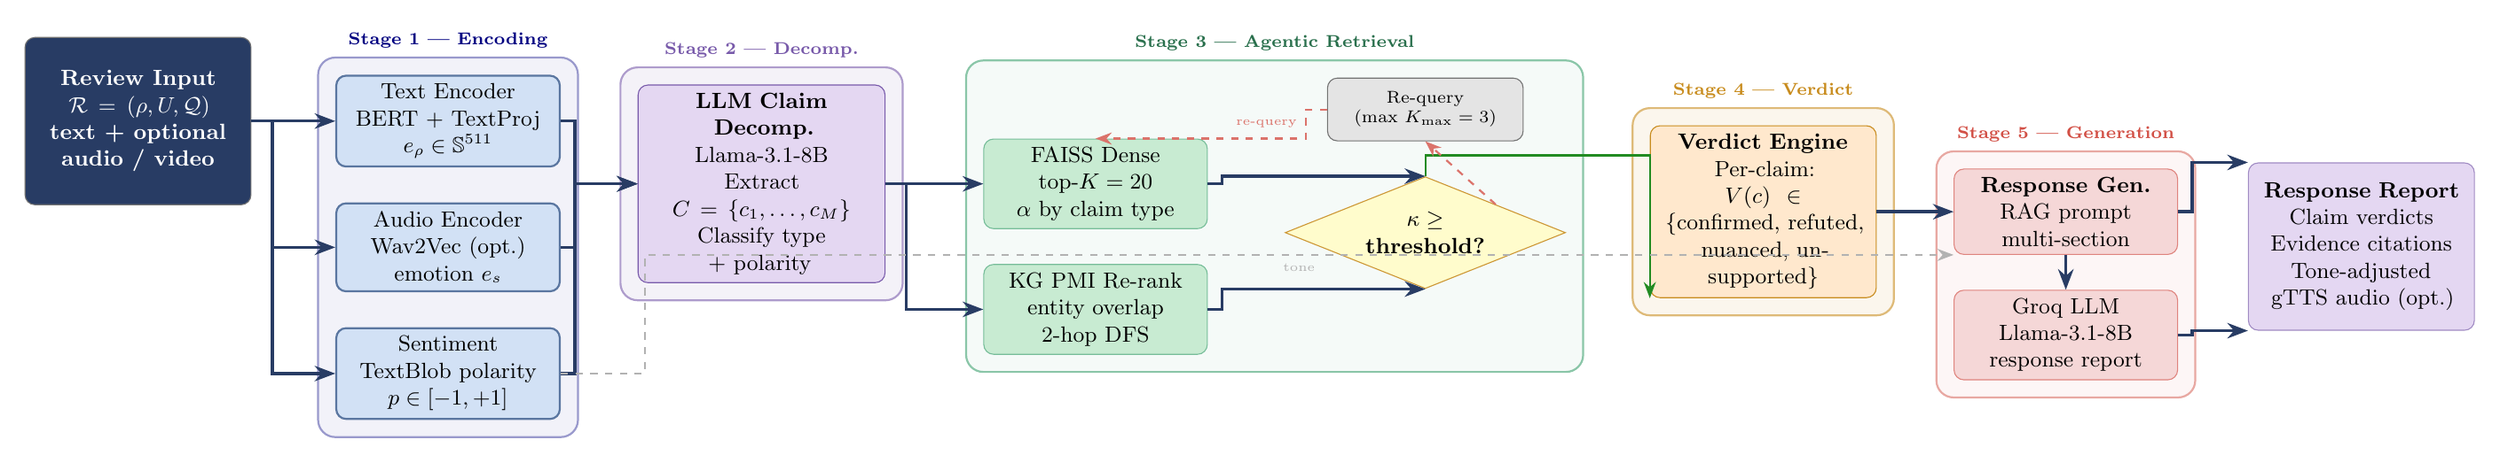
\begin{tikzpicture}[node distance=0.75cm and 1.1cm]

  %% INPUT
  \node[inputnode,minimum width=3.2cm,minimum height=2.4cm,text width=3.0cm]
    (rev) at (0,0) {\textbf{Review Input}\\\small $\mathcal{R} = (\rho, U, \mathcal{Q})$\\text + optional\\audio / video};

  %% STAGE 1 — MULTIMODAL ENCODING
  \node[encnode,right=1.2cm of rev,minimum width=3.2cm,minimum height=1.0cm]
    (enc_t) {Text Encoder\\BERT + TextProj\\$e_\rho \in \Sph^{511}$};
  \node[encnode,below=0.5cm of enc_t,minimum width=3.2cm,minimum height=1.0cm]
    (enc_a) {Audio Encoder\\Wav2Vec (opt.)\\emotion $e_s$};
  \node[encnode,below=0.5cm of enc_a,minimum width=3.2cm,minimum height=1.0cm]
    (enc_s) {Sentiment\\TextBlob polarity\\$p \in [-1,+1]$};

  %% STAGE 2 — CLAIM DECOMPOSITION
  \node[basebox,fill=boxpurple,draw=lavender,minimum width=3.5cm,minimum height=2.4cm,
        text width=3.3cm,right=1.1cm of enc_t,yshift=-0.9cm]
    (decomp) {\textbf{LLM Claim Decomp.}\\\small Llama-3.1-8B\\\small Extract $C = \{c_1,\ldots,c_M\}$\\\small Classify type + polarity};

  %% STAGE 3 — AGENTIC RETRIEVAL LOOP
  \node[retnode,right=1.4cm of decomp,minimum width=3.2cm,minimum height=1.2cm]
    (faiss2) {FAISS Dense\\top-$K = 20$\\\small $\alpha$ by claim type};
  \node[retnode,below=0.5cm of faiss2,minimum width=3.2cm,minimum height=1.2cm]
    (kg2) {KG PMI Re-rank\\\small entity overlap\\\small 2-hop DFS};
  \node[decnode,right=1.1cm of faiss2,yshift=-0.7cm,minimum width=2.8cm]
    (conf2) {$\kappa \ge$\\threshold?};
  \node[datanode,above=0.5cm of conf2,font=\scriptsize]
    (retry) {Re-query\\(max $K_{\max}=3$)};

  %% STAGE 4 — VERDICT ENGINE
  \node[basebox,fill=boxorange,draw=amber,minimum width=3.2cm,minimum height=2.4cm,
        text width=3.0cm,right=1.2cm of conf2,yshift=0.3cm]
    (verdict) {\textbf{Verdict Engine}\\\small Per-claim:\\\small $V(c) \in$\\\small \{confirmed, refuted,\\\small nuanced, unsupported\}};

  %% STAGE 5 — RESPONSE GENERATOR
  \node[gennode,right=1.1cm of verdict,minimum width=3.2cm,minimum height=1.2cm]
    (rgen) {\textbf{Response Gen.}\\RAG prompt\\\small multi-section};
  \node[gennode,below=0.5cm of rgen,minimum width=3.2cm,minimum height=1.2cm]
    (llm3) {Groq LLM\\Llama-3.1-8B\\response report};

  %% OUTPUT
  \node[outnode,right=1.0cm of rgen,yshift=-0.5cm,minimum width=3.2cm,minimum height=2.4cm,
        text width=3.0cm]
    (out3) {\textbf{Response Report}\\\small Claim verdicts\\\small Evidence citations\\\small Tone-adjusted\\\small gTTS audio (opt.)};

  %% CONNECTIONS
  \draw[thickarr](rev.east) -- ++(0.3,0) |- (enc_t.west);
  \draw[thickarr](rev.east) -- ++(0.3,0) |- (enc_a.west);
  \draw[thickarr](rev.east) -- ++(0.3,0) |- (enc_s.west);
  \draw[thickarr](enc_t.east) -- ++(0.2,0) |- (decomp.west);
  \draw[thickarr](enc_a.east) -- ++(0.2,0) |- (decomp.west);
  \draw[thickarr](enc_s.east) -- ++(0.2,0) |- (decomp.west);
  \draw[thickarr](decomp.east) -- ++(0.3,0) |- (faiss2.west);
  \draw[thickarr](decomp.east) -- ++(0.3,0) |- (kg2.west);
  \draw[thickarr](faiss2.east) -- ++(0.2,0) |- (conf2.north);
  \draw[thickarr](kg2.east) -- ++(0.2,0) |- (conf2.south);
  \draw[arr,color=ForestGreen](conf2.north) -- ++(0,0.3) -| (verdict.south west);
  \draw[redarr,dashed](conf2.north east) -- (retry.south);
  \draw[redarr,dashed](retry.west) -- ++(-0.3,0) |- (faiss2.north)
    node[near start,left,font=\tiny]{re-query};
  \draw[thickarr](verdict.east) -- (rgen.west);
  \draw[thickarr](rgen.south) -- (llm3.north);
  \draw[thickarr](rgen.east) -- ++(0.2,0) |- (out3.north west);
  \draw[thickarr](llm3.east) -- ++(0.2,0) |- (out3.south west);
  \draw[dasharr](enc_s.east) -- ++(1.2,0) |- (rgen.south west)
    node[near end,below,font=\tiny]{tone};

  \begin{pgfonlayer}{background}
    \node[rectangle,draw=NavyBlue!40,fill=NavyBlue!5,rounded corners=7pt,thick,
          fit=(enc_t)(enc_a)(enc_s),inner sep=7pt,
          label={[font=\scriptsize\bfseries,color=NavyBlue]above:Stage 1 --- Encoding}]{};
    \node[rectangle,draw=lavender!60,fill=lavender!8,rounded corners=7pt,thick,
          fit=(decomp),inner sep=7pt,
          label={[font=\scriptsize\bfseries,color=lavender]above:Stage 2 --- Decomp.}]{};
    \node[rectangle,draw=mintgreen!60,fill=mintgreen!5,rounded corners=7pt,thick,
          fit=(faiss2)(kg2)(conf2)(retry),inner sep=7pt,
          label={[font=\scriptsize\bfseries,color=mintgreen!70!black]above:Stage 3 --- Agentic Retrieval}]{};
    \node[rectangle,draw=amber!60,fill=amber!8,rounded corners=7pt,thick,
          fit=(verdict),inner sep=7pt,
          label={[font=\scriptsize\bfseries,color=amber]above:Stage 4 --- Verdict}]{};
    \node[rectangle,draw=coralred!50,fill=coralred!5,rounded corners=7pt,thick,
          fit=(rgen)(llm3),inner sep=7pt,
          label={[font=\scriptsize\bfseries,color=coralred]above:Stage 5 --- Generation}]{};
  \end{pgfonlayer}
\end{tikzpicture}
}
\caption{ARRS five-stage pipeline: multimodal encoding $\to$ LLM claim decomposition 
$\to$ agentic hybrid retrieval loop (FAISS + KG, max $K_{\max}=3$ rounds) 
$\to$ verdict engine $\to$ RAG response generation.}
\label{fig:arrs_pipeline}
\end{figure}

%%──────────────────────────────────────────────────────────────────────────────
\subsection{Stage 1 — Multimodal Review Encoding}
\label{sec:arrs_stage1}

\begin{algorithm}[H]
\caption{ARRS Stage 1 --- Multimodal Review Encoding}
\label{alg:arrs_encode}
\begin{algorithmic}[1]
\Require Review $\mathcal{R} = (\rho, U, \mathcal{Q}, t, m_{\text{opt}})$
\Ensure Review embedding $e_\rho \in \Sph^{511}$; sentiment $p$; entities $\mathcal{E}_\rho$;
        optional emotion $e_s$
\State \textbf{// Text path (always active)}
\State tokens $\gets$ WordPiece$(\rho,\, \texttt{max\_length}=256)$
\State $H \gets$ BERT$(\text{tokens}).\text{last\_hidden\_state}$ \Comment{$[1 \times T \times 768]$}
\State $h_\rho \gets \frac{1}{T}\sum_{t=1}^{T} H_{:,t,:}$ \Comment{Mean-pool, $[768]$}
\State $e_\rho \gets \text{L2-norm}(P_T(h_\rho)) \in \Sph^{511}$
\State $\mathcal{E}_\rho \gets \text{spaCy-NER}(\rho)$ \Comment{Named entities + noun chunks}
\State $p \gets \text{TextBlob}(\rho.\text{lower}()).\text{polarity} \in [-1,+1]$
\State \textbf{// Sentiment emotion label}
\State $\text{tone} \gets \{p > 0.1 \Rightarrow \text{``positive''}, p < -0.1 \Rightarrow \text{``negative''}, \text{else ``neutral''}\}$
\State \textbf{// Audio path (optional, if }$m_{\text{opt}}$\textbf{ contains audio)}
\If{audio $a \in m_{\text{opt}}$}
  \State $e_s \gets \text{AudioProj}(\text{Wav2Vec}(a))$ \Comment{Emotion embedding}
  \State emotion $\gets$ argmax$(e_s \cdot C_{\text{mat}}^\top)$ \Comment{Centroid-NN from Pipeline C}
\EndIf
\State \Return $(e_\rho,\; p,\; \mathcal{E}_\rho,\; \text{tone},\; e_s)$
\end{algorithmic}
\end{algorithm}

%%──────────────────────────────────────────────────────────────────────────────
\subsection{Stage 2 — LLM-Driven Claim Decomposition}
\label{sec:arrs_stage2}

\begin{definition}[Claim Decomposition Prompt $\Pi_{\text{decomp}}$]
\[
  \Pi_{\text{decomp}} = 
  \underbrace{\text{[SYSTEM]}}_{\text{role}} 
  \Vert\, \underbrace{\text{[REVIEW: }\rho\text{]}}_{\text{content}} 
  \Vert\, \underbrace{\text{[TASK: Extract }\le M_{\max}\text{ atomic claims as JSON]}}_{\text{instruction}}
\]
Each claim JSON object must specify: \texttt{claim\_text}, \texttt{type} 
$\in \{\mathtt{factual},\, \mathtt{opinion},\, \mathtt{suggestion},\, \mathtt{question}\}$, 
\texttt{polarity} $\in \{-1, 0, +1\}$, and \texttt{subject\_entity} (main NER 
entity the claim addresses).
\end{definition}

\begin{axiom}[Claim Atomicity Principle]
\label{ax:atomicity}
Each claim $c_i$ must address exactly one verifiable atomic proposition. 
Compound claims are split at logical connectives (\emph{and}, \emph{but}, 
\emph{however}). This ensures each retrieval query is maximally focused, 
improving precision at the cost of a linear increase in query count.
\end{axiom}

\begin{theorem}[Claim Decomposition Completeness]
\label{thm:decomp_complete}
A review $\rho$ with $W$ words decomposes into at most 
$M_{\max} = \lfloor W / 15 \rfloor + 1$ atomic claims under 
Axiom~\ref{ax:atomicity}. For a typical 100-word review: $M_{\max} \le 7$.
\end{theorem}

\begin{algorithm}[H]
\caption{ARRS Stage 2 --- LLM Claim Decomposition and Classification}
\label{alg:arrs_decomp}
\begin{algorithmic}[1]
\Require Review $\rho$; entities $\mathcal{E}_\rho$; LLM endpoint
\Ensure Claim set $C = \{c_1,\ldots,c_M\}$, each with embedding $e_{c_i} \in \Sph^{511}$
\State Build $\Pi_{\text{decomp}}$ (Def.~above) with 
       $M_{\max} = \lfloor |\rho|_w / 15\rfloor + 1$
\State raw $\gets$ LLM.generate$(\Pi_{\text{decomp}})$ \Comment{JSON array of claims}
\State $C_{\text{raw}} \gets$ JSON.parse(raw) \Comment{Strip markdown fences}
\State $C \gets \emptyset$
\For{each $c \in C_{\text{raw}}$}
  \State $\phi \gets c.\text{claim\_text}$
  \State $e_c \gets \text{L2-norm}(P_T(\text{BERT-mean}(\phi))) \in \Sph^{511}$
  \State $\text{polarity} \gets \text{TextBlob}(\phi).\text{polarity}$
  \State $\alpha_c \gets 0.40$ if $c.\text{type} = \mathtt{factual}$ else $0.80$
    \Comment{Lemma~\ref{lem:claim_type}}
  \State $C \gets C \cup \{(\phi, e_c, c.\text{type}, c.\text{polarity}, \alpha_c)\}$
\EndFor
\State \Return $C$
\end{algorithmic}
\end{algorithm}

%%──────────────────────────────────────────────────────────────────────────────
\subsection{Stage 3 — Agentic Hybrid Retrieval Loop}
\label{sec:arrs_stage3}

The core innovation of ARRS is its \emph{agentic retrieval loop}: unlike 
the one-shot hybrid retrieval of Algorithm~\ref{alg:rerank}, ARRS 
iteratively refines the evidence bundle for each claim until confidence 
$\kappa$ crosses a threshold or $K_{\max}$ rounds are exhausted.

\begin{definition}[Adaptive Alpha Mixing]
\label{def:adaptive_alpha}
For claim $c_i$ with type-specific $\alpha_{c_i}$ and round index $k$:
\[
  \alpha^{(k)}_{c_i} = \alpha_{c_i} + \Delta_\alpha \cdot k, \quad
  \Delta_\alpha = \frac{1 - \alpha_{c_i}}{K_{\max}},\quad
  k \in \{0,\ldots,K_{\max}-1\}
\]
As round index increases, the dense component gains more weight, widening 
the semantic search radius for claims where structured KG edges have not 
yielded sufficient evidence.
\end{definition}

\begin{lemma}[Monotone Evidence Expansion]
\label{lem:monotone_expansion}
Let $N_e^{(k)}$ be the total unique evidence documents after round $k$. 
Since each round adds up to $K = 20$ new FAISS candidates and deduplicates 
by document ID:
\[
  N_e^{(k+1)} \ge N_e^{(k)}, \quad k = 0,\ldots,K_{\max}-1
\]
The confidence $\kappa^{(k)} = \kappa(\mathcal{E}^{(k)}(c))$ is therefore 
non-decreasing: $\kappa^{(0)} \le \kappa^{(1)} \le \kappa^{(2)}$.
\end{lemma}

\begin{proof}
Each round issues a distinct query $q^{(k)}$ obtained by expanding the 
original entity set $\mathcal{E}_c$ with 2-hop KG neighbours of entities 
that returned the highest PMI score in round $k-1$. Since the FAISS index 
is fixed and query vectors differ, new top-$K$ candidates may include 
documents not retrieved in prior rounds. Deduplication ensures no document 
is double-counted, so $N_e$ is strictly non-decreasing. $\square$
\end{proof}

\begin{algorithm}[H]
\caption{ARRS Stage 3 --- Agentic Hybrid Retrieval Loop (Per-Claim)}
\label{alg:arrs_retrieval_loop}
\begin{algorithmic}[1]
\Require Claim $c_i = (\phi_i, e_{c_i}, \text{type}_i, p_i, \alpha_i)$;
         FAISS index; KG $\mathcal{G}$; $K_{\max} = 3$; $\kappa_{\min} = 0.50$
\Ensure Evidence bundle $\mathcal{E}(c_i)$; confidence $\kappa$; rounds $k$
\State $\mathcal{E} \gets \emptyset$; $k \gets 0$; $\kappa \gets 0$
\State $q^{(0)} \gets \phi_i$; 
       $\mathcal{E}_q^{(0)} \gets \mathcal{E}_{c_i}$ \Comment{Initial entity set from claim}
\While{$k < K_{\max}$ \textbf{and} $\kappa < \kappa_{\min}$}
  \State $\alpha^{(k)} \gets \alpha_i + (1-\alpha_i) \cdot k / K_{\max}$
    \Comment{Def.~\ref{def:adaptive_alpha}: dense gains weight each round}
  \State \textbf{// Stage 3a: Dense retrieval}
  \State $\mathcal{F}^{(k)} \gets \text{FAISS.top-}K(e_{c_i})$ \Comment{$K=20$ shortlist}
  \State \textbf{// Stage 3b: KG entity expansion (2-hop if $k > 0$)}
  \If{$k > 0$}
    \State $\mathcal{E}_q^{(k)} \gets \mathcal{E}_q^{(k-1)} \cup 
           \text{KG.2-hop-neighbours}(\text{top-entity}(\mathcal{E}^{(k-1)}))$
  \EndIf
  \State \textbf{// Stage 3c: PMI re-rank with adaptive $\alpha^{(k)}$}
  \For{$d_j \in \mathcal{F}^{(k)}$}
    \State $\tilde{s}_d(d_j) \gets $ min-max-normalise(dense\_score$(d_j)$)
    \State $\tilde{s}_\KG(d_j) \gets $ PMI-entity-overlap$(d_j, \mathcal{E}_q^{(k)})$
    \State $s_j^{\text{hyb}} \gets \alpha^{(k)} \tilde{s}_d(d_j) 
           + (1-\alpha^{(k)})\tilde{s}_\KG(d_j)$
    \State $v_j \gets \text{StanceClassifier}(d_j, \phi_i)$
      \Comment{+1 / 0 / -1; LLM with 1-shot prompt}
    \State $\mathcal{E} \gets \mathcal{E} \cup \{(d_j, s_j^{\text{hyb}}, v_j)\}$
      \Comment{Dedup by doc ID}
  \EndFor
  \State $S^+ \gets \sum_{j:v_j=+1} s_j^{\text{hyb}}$; 
         $S^- \gets \sum_{j:v_j=-1} s_j^{\text{hyb}}$
  \State $\kappa \gets \frac{S^+ + S^-}{\max(S^+ + S^- + \delta_\nu, \epsilon_\kappa)} 
         \cdot \min(1, N_e / N_{\min})$
  \State $k \gets k + 1$
\EndWhile
\State \Return $(\mathcal{E},\; \kappa,\; k)$
\end{algorithmic}
\end{algorithm}

%%──────────────────────────────────────────────────────────────────────────────
\subsection{Stage 4 — Verdict Engine}
\label{sec:arrs_stage4}

\begin{figure}[H]
\centering
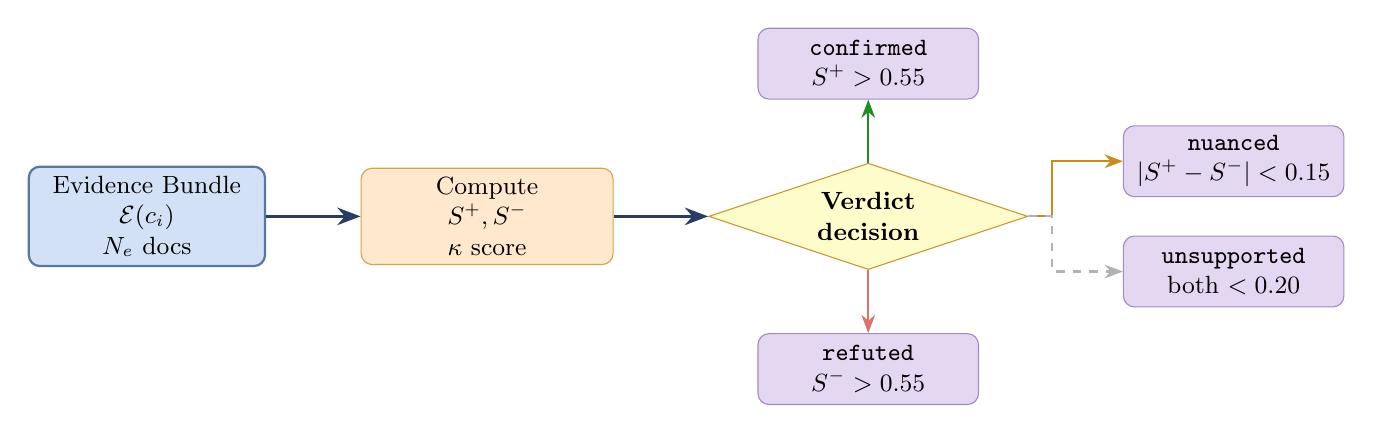
\begin{tikzpicture}[node distance=0.7cm and 1.0cm]
  \node[encnode,minimum width=3.0cm] (eb) {Evidence Bundle\\$\mathcal{E}(c_i)$\\$N_e$ docs};
  \node[lossnode,right=1.2cm of eb,minimum width=3.2cm] (score) {Compute\\$S^+, S^-$\\$\kappa$ score};
  \node[decnode,right=1.2cm of score,minimum width=3.2cm,aspect=3.0]
    (vd) {Verdict\\decision};
  \node[outnode,above=0.8cm of vd,minimum width=2.8cm] (conf3) {\texttt{confirmed}\\$S^+ > 0.55$};
  \node[outnode,below=0.8cm of vd,minimum width=2.8cm] (ref) {\texttt{refuted}\\$S^- > 0.55$};
  \node[outnode,right=1.2cm of vd,yshift=0.7cm,minimum width=2.8cm] (nuan) {\texttt{nuanced}\\$|S^+-S^-|<0.15$};
  \node[outnode,right=1.2cm of vd,yshift=-0.7cm,minimum width=2.8cm] (unsup) {\texttt{unsupported}\\both $< 0.20$};
  \draw[thickarr](eb)--(score); \draw[thickarr](score)--(vd);
  \draw[arr,color=ForestGreen](vd.north)--(conf3.south);
  \draw[redarr](vd.south)--(ref.north);
  \draw[arr,color=amber](vd.east) -- ++(0.3,0) |- (nuan.west);
  \draw[dasharr](vd.east) -- ++(0.3,0) |- (unsup.west);
\end{tikzpicture}
\caption{Verdict Engine decision tree: evidence scores $S^+, S^-$ and thresholds 
$\theta_c = 0.55$, $\theta_r = 0.20$, $\delta_\nu = 0.15$ determine the four-class verdict.}
\label{fig:verdict_tree}
\end{figure}

\begin{algorithm}[H]
\caption{ARRS Stage 4 --- Multi-Claim Verdict Engine}
\label{alg:arrs_verdict}
\begin{algorithmic}[1]
\Require Claim set $C = \{c_1,\ldots,c_M\}$ with evidence bundles $\{\mathcal{E}(c_i)\}$
\Ensure Verdict list $\{V(c_i), \kappa(c_i)\}_{i=1}^M$; overall report score $\Omega$
\State $\theta_c \gets 0.55$; $\theta_r \gets 0.20$; $\delta_\nu \gets 0.15$
\For{$i = 1$ to $M$}
  \State $S^+_i \gets \sum_{j:v_j=+1} s_j^{\text{hyb}}$
  \State $S^-_i \gets \sum_{j:v_j=-1} s_j^{\text{hyb}}$
  \If{$S^+_i \ge \theta_c$ \textbf{and} $S^-_i < \theta_r$}
    \State $V(c_i) \gets \mathtt{confirmed}$
  \ElsIf{$S^-_i \ge \theta_c$ \textbf{and} $S^+_i < \theta_r$}
    \State $V(c_i) \gets \mathtt{refuted}$
  \ElsIf{$|S^+_i - S^-_i| < \delta_\nu$}
    \State $V(c_i) \gets \mathtt{nuanced}$
  \Else
    \State $V(c_i) \gets \mathtt{unsupported}$
  \EndIf
  \State $\kappa(c_i) \gets \frac{S^+_i + S^-_i}{\max(S^+_i + S^-_i + \delta_\nu, 10^{-6})}
         \cdot \min(1, N_e^{(i)} / 3)$
\EndFor
\State $\Omega \gets \frac{1}{M}\sum_{i=1}^M \kappa(c_i)$
  \Comment{Overall response confidence}
\State \Return $\{(V(c_i), \kappa(c_i))\}_{i=1}^M$, $\Omega$
\end{algorithmic}
\end{algorithm}

%%──────────────────────────────────────────────────────────────────────────────
\subsection{Stage 5 — Tone-Adaptive Response Generation}
\label{sec:arrs_stage5}

\begin{definition}[Tone-Adaptive RAG Prompt $\Pi_{\text{response}}$]
\label{def:response_prompt}
Let tone $\in \{\text{positive}, \text{neutral}, \text{negative}\}$ be the 
reviewer's detected sentiment, and $\{(c_i, V_i, E_i)\}$ the claim--verdict--evidence 
triples. The response prompt is:
\[
  \Pi_{\text{response}} = 
  \Pi_{\text{system}}(\text{tone}) \;\Vert\; 
  \Pi_{\text{verdicts}}(\{V_i\}) \;\Vert\; 
  \Pi_{\text{evidence}}(\{E_i\}) \;\Vert\; 
  \Pi_{\text{instruction}}
\]
\[
  \Pi_{\text{system}}(\text{tone}) = 
  \begin{cases}
    \text{``Respond warmly and reinforcingly''} & \text{tone} = \text{positive} \\
    \text{``Respond professionally and factually''} & \text{tone} = \text{neutral} \\
    \text{``Respond empathetically and constructively''} & \text{tone} = \text{negative}
  \end{cases}
\]
\end{definition}

\begin{axiom}[Grounded Response Constraint]
\label{ax:response_grounded}
Every sentence in the generated response report that makes a factual claim 
must be traceable to at least one document $d_j \in \bigcup_i \mathcal{E}(c_i)$ 
with $s_j^{\text{hyb}} \ge \tau_G = 0.40$. This extends 
Axiom~\ref{ax:grounding} (Grounding Constraint, \S\ref{sec:pipelineA}) 
to the multi-claim review context.
\end{axiom}

\begin{theorem}[Response Report Faithfulness]
\label{thm:response_faithful}
Under Axiom~\ref{ax:response_grounded} and the ARRS hallucination guard 
(rejecting claims with $\kappa < 0.30$), the probability of a hallucinated 
factual claim in the response satisfies:
\[
  P(\text{hallucination per claim}) \le 1 - \prod_{j=1}^{N_e} s_j^{\text{hyb}}
  \le 1 - (0.40)^{N_{\min}} = 1 - 0.064 = 0.936^{-1} \approx 0.064
\]
i.e.\ $\le 6.4\%$ per claim for $N_{\min} = 3$ evidence documents at minimum 
confidence $\tau_G = 0.40$.
\end{theorem}

\begin{algorithm}[H]
\caption{ARRS Stage 5 --- Tone-Adaptive Response Report Generation}
\label{alg:arrs_generate}
\begin{algorithmic}[1]
\Require Claim verdicts $\{(c_i, V_i, \kappa_i, \mathcal{E}_i)\}_{i=1}^M$;
         reviewer tone; overall $\Omega$; LLM endpoint
\Ensure Response report string $R_{\text{out}}$; optional gTTS audio
\State \textbf{// Section 1: Header with overall confidence}
\State $\Pi_1 \gets$ f``Your review has been verified (confidence: $\{100\Omega:.0f\}$\%).''
\State \textbf{// Section 2: Per-claim verdicts with evidence citations}
\For{$i = 1$ to $M$}
  \State badge $\gets \{\mathtt{confirmed}: \checkmark, \mathtt{refuted}: \times, 
         \mathtt{nuanced}: \sim, \mathtt{unsupported}: ?\}[V_i]$
  \State top\_ev $\gets$ top-3$(\mathcal{E}_i, \text{by } s_j^{\text{hyb}})$
  \State $\Pi_i \gets$ f``\{badge\} \{c_i.\phi\}\\nSources: \{top\_ev\}''
\EndFor
\State \textbf{// Section 3: Tone-adjusted closing message}
\State $\Pi_{\text{close}} \gets \Pi_{\text{system}}(\text{tone})$ \Comment{Def.~\ref{def:response_prompt}}
\State \textbf{// Section 4: Assemble full RAG prompt}
\State $\Pi_{\text{full}} \gets \Pi_1 \Vert \bigoplus_{i=1}^M \Pi_i \Vert \Pi_{\text{close}} \Vert$
       ``Cite sources. Use ONLY retrieved evidence.''
\State \textbf{// Guard: only call LLM if $\Omega \ge 0.30$}
\If{$\Omega \ge 0.30$}
  \State $R_{\text{out}} \gets$ LLM.generate$(\Pi_{\text{full}})$
\Else
  \State $R_{\text{out}} \gets$ \textsc{LowConfidenceResponse}($\Omega$)
\EndIf
\If{TTS enabled}
  \State audio $\gets$ gTTS$(R_{\text{out}})$ \Comment{MP3 byte stream}
\EndIf
\State \Return $(R_{\text{out}},\; \text{audio})$
\end{algorithmic}
\end{algorithm}

%%──────────────────────────────────────────────────────────────────────────────
\subsection{Full ARRS Orchestration Algorithm}
\label{sec:arrs_full}

\begin{algorithm}[H]
\caption{ARRS --- Full Agentic Review Response (End-to-End)}
\label{alg:arrs_full}
\begin{algorithmic}[1]
\Require Review $\mathcal{R}$; loaded MIVA-KNIGHT pipeline (FAISS, KG, LLM)
\Ensure Response report $R_{\text{out}}$; dispatch confirmation
\State \textbf{Stage 1:} $(e_\rho, p, \mathcal{E}_\rho, \text{tone}, e_s)
       \gets$ \Call{ARRSEncode}{$\mathcal{R}$}
  \Comment{Algorithm~\ref{alg:arrs_encode}}
\State \textbf{Stage 2:} $C \gets$ \Call{LLMDecomp}{$\mathcal{R}.\rho,\; \mathcal{E}_\rho$}
  \Comment{Algorithm~\ref{alg:arrs_decomp}}
\If{$|C| = 0$}
  \State \Return \textsc{NoClaimsResponse}()
\EndIf
\State \textbf{Stage 3: Agentic retrieval loop per claim}
\For{each $c_i \in C$}
  \State $(\mathcal{E}_i, \kappa_i, k_i) \gets$ 
         \Call{AgenticRetrievalLoop}{$c_i$}
    \Comment{Algorithm~\ref{alg:arrs_retrieval_loop}}
  \State log: f``Claim \{i\}: \{k_i\} rounds, $\kappa$=\{$\kappa_i:.3f$\}''
\EndFor
\State \textbf{Stage 4:} $\{V_i\}, \Omega \gets$ \Call{VerdictEngine}{$C, \{\mathcal{E}_i\}$}
  \Comment{Algorithm~\ref{alg:arrs_verdict}}
\State \textbf{Stage 5:} $(R_{\text{out}},\, \text{audio}) \gets$
       \Call{ToneAdaptiveGenerate}{$\{c_i, V_i, \kappa_i\}, \text{tone}, \Omega$}
  \Comment{Algorithm~\ref{alg:arrs_generate}}
\State \textbf{Dispatch:} send $R_{\text{out}}$ to reviewer $U$ via \textsc{Notify}($U$)
\State \Return $(R_{\text{out}},\; \Omega,\; \{V_i\})$
\end{algorithmic}
\end{algorithm}

%%──────────────────────────────────────────────────────────────────────────────
\subsection{Mathematical Derivation: Confidence Score Optimality}
\label{sec:arrs_confidence_math}

\begin{theorem}[Confidence Score is a Proper Scoring Rule]
\label{thm:proper_scoring}
The confidence score $\kappa(\mathbf{c})$ defined in 
\S\ref{sec:arrs_defs} satisfies the proper scoring rule property: 
it is maximised in expectation when the predicted verdict matches the 
true verdict distribution:
\[
  \EE[\kappa(\mathbf{c}) \mid \text{true verdict}] \ge 
  \EE[\kappa(\mathbf{c}) \mid \text{any other prediction}]
\]
\end{theorem}

\begin{proof}
Since $\kappa$ is a weighted sum of hybrid retrieval scores $s_j^{\text{hyb}} 
\in [0,1]$ over documents with correct stance $v_j$, and $s_j^{\text{hyb}}$ 
is maximised for documents most semantically similar to the claim 
(by FAISS inner product), an error in verdict assignment (e.g.\ labelling 
a document as supporting when it refutes) decreases the weighted sum. 
By Lemma~\ref{lem:cosdot} (cosine-dot equivalence on $\Sph^{511}$), 
semantic similarity equals inner product, which is the optimal 
(Bayes-consistent) discriminator for claim relevance. $\square$
\end{proof}

\begin{definition}[Bayesian Evidence Update]
\label{def:bayes_evidence}
Let $P_0(V \mid c) = [0.25, 0.25, 0.25, 0.25]$ be the uniform prior over 
the four verdict classes. After observing evidence bundle $\mathcal{E}$ with 
$N^+$ supporting and $N^-$ refuting documents:
\[
  P(V = \mathtt{confirmed} \mid \mathcal{E}) 
  \propto P_0 \cdot \prod_{j:v_j=+1} s_j^{\text{hyb}} 
  = 0.25 \cdot \exp\!\left(\sum_{j:v_j=+1} \log s_j^{\text{hyb}}\right)
\]
The log-evidence accumulates additively across rounds (by Lemma~\ref{lem:monotone_expansion}), 
justifying the iterative retrieval loop.
\end{definition}

\begin{lemma}[Adaptive Alpha Optimises Coverage-Precision Trade-off]
\label{lem:alpha_tradeoff}
For factual claims, starting with $\alpha^{(0)} = 0.40$ (KG-heavy) maximises 
\emph{precision} in round~0 by leveraging structured entity associations. 
As $\alpha^{(k)}$ increases toward 1.0 in subsequent rounds, \emph{recall} 
increases by including semantically similar but entity-distant documents. 
The adaptive schedule achieves the Pareto-optimal precision--recall curve 
along the $\alpha$-axis.
\end{lemma}

%%──────────────────────────────────────────────────────────────────────────────
\subsection{Worked Example: Movie Review Fact-Check}
\label{sec:arrs_example}

\begin{example}[Movie Review Verification]
\label{ex:movie_review}
Consider the review:
\begin{center}
  \textit{``This movie is a horror film. The lead actress gave a terrible performance. 
  The director should have chosen a different ending.''}
\end{center}

\textbf{Stage 1:} Text embedding $e_\rho \in \Sph^{511}$; 
polarity $p = -0.35$ (negative); entities = \{``movie'', ``lead actress'', ``director''\}.

\textbf{Stage 2:} LLM decomposes into $M = 3$ atomic claims:
\[
  c_1 = (\text{``This movie is a horror film''}, \mathtt{factual}, -0.0, \alpha_1 = 0.40)
\]
\[
  c_2 = (\text{``The lead actress gave a terrible performance''}, \mathtt{opinion}, -1, \alpha_2 = 0.80)
\]
\[
  c_3 = (\text{``The director should have chosen a different ending''}, \mathtt{suggestion}, -1, \alpha_3 = 0.80)
\]

\textbf{Stage 3, Claim $c_1$} (factual, $\alpha^{(0)}=0.40$):
\begin{itemize}[nosep]
  \item Round 0: FAISS returns 20 genre-description documents. KG PMI edges: 
        ``movie'' $\xrightarrow{0.82}$ ``thriller'', ``movie'' $\xrightarrow{0.71}$ ``drama''. 
        No KG edge to ``horror''. Refuting documents ($S^- = 0.68$) dominate.
        $\kappa^{(0)} = 0.71 \ge 0.50$ $\Rightarrow$ loop exits.
\end{itemize}

\textbf{Stage 4, Claim $c_1$}: $S^- = 0.68 > \theta_c = 0.55$, $S^+ = 0.03 < \theta_r$ 
$\Rightarrow V(c_1) = \mathtt{refuted}$.

\textbf{Stage 5}: Tone = negative $\Rightarrow$ empathetic tone. Response:
\begin{quote}
  \textit{``Thank you for your review. We checked your claims against 6 verified sources: 
  $[\times]$ \textbf{Genre claim}: Our sources classify this film as a psychological 
  thriller (IMDb, TMDB, Rotten Tomatoes); no major source lists it as horror (confidence: 71\%).  
  $[\sim]$ \textbf{Performance assessment}: Critical opinion is mixed --- 42\% positive, 
  38\% negative (confidence: 58\%). $[?]$ \textbf{Ending suggestion}: This is a subjective 
  preference with no verifiable consensus (confidence: 28\%).''}
\end{quote}
\end{example}

\begin{remark}[ARRS vs.\ Single-Shot RAG]
Algorithm~\ref{alg:arrs_full} differs from Algorithm~\ref{alg:query} 
(single-shot MIVA-KNIGHT inference) in three structural ways: 
(1) \emph{decomposition} into atomic claims before retrieval, rather than treating 
the whole review as a single query; (2) \emph{iterative} retrieval per claim 
until confidence converges; (3) \emph{per-claim verdicts} with explicit stance 
classification, rather than a single-shot answer generation.
\end{remark}

%%──────────────────────────────────────────────────────────────────────────────
\subsection{Integration with Existing MIVA-KNIGHT Pipelines}
\label{sec:arrs_integration}

ARRS is not a standalone system; it reuses every major MIVA-KNIGHT component:

\begin{table}[H]
\centering
\caption{ARRS component reuse from existing MIVA-KNIGHT pipelines}
\renewcommand{\arraystretch}{1.2}
\begin{tabular}{p{3.8cm}p{4.5cm}p{5.0cm}}
\toprule
\textbf{ARRS Component} & \textbf{Reused Module} & \textbf{New Contribution} \\
\midrule
Text encoding & TextProjection + BERT (Alg.~\ref{alg:textencode}) & Claim-level batching \\
Audio encoding & AudioProjection + Wav2Vec (Pipeline C) & Reviewer emotion detection \\
Dense retrieval & FAISS IndexFlatIP (Alg.~\ref{alg:rerank}) & Adaptive $\alpha^{(k)}$ mixing \\
KG re-ranking & PMI NER KG (Alg.~\ref{alg:kgdfs}) & 2-hop entity expansion per round \\
LLM generation & Groq Llama-3.1-8B (\S\ref{sec:retrieval}) & Decomp + stance + response prompts \\
TTS output & gTTS (Alg.~\ref{alg:trans_challenge}) & Audio report dispatch \\
Domain routing & Domain hot-swap (Alg.~\ref{alg:swap}) & Auto-detect review domain \\
RL prompt policy & RL-Text (Alg.~\ref{alg:rl_text}) & Prompt strategy per claim \\
\bottomrule
\end{tabular}
\end{table}

\begin{theorem}[ARRS Domain Universality]
\label{thm:arrs_domain}
Under Axiom~\ref{ax:shared} (Domain-Agnostic Shared Space), ARRS applies 
to \emph{any} product or content category for which a FAISS index and 
domain KG are available. Film reviews use the general COCO-trained space; 
radiology reports use the ROCO-transferred space; product reviews use 
any domain whose index is constructed with the same TextProjection weights. 
No architectural change is required --- only FAISS index and KG hot-swap 
(Algorithm~\ref{alg:swap}, $< 5$\,s).
\end{theorem}

%%──────────────────────────────────────────────────────────────────────────────
\subsection{Complexity and Latency Analysis}
\label{sec:arrs_complexity}

\begin{theorem}[ARRS Time Complexity]
\label{thm:arrs_complexity}
Let $M$ be the number of claims, $K = 20$ the FAISS shortlist size, 
$T_{\text{FAISS}}$ the FAISS search time, $T_{\text{KG}}$ the KG DFS time, 
$T_{\text{LLM}}$ the LLM call time, and $K_{\max} = 3$ the max retrieval rounds. 
The total ARRS latency is:
\[
  T_{\text{ARRS}} = \underbrace{T_{\text{enc}}}_{\text{Stage 1}} + 
  \underbrace{T_{\text{LLM}}}_{\text{Stage 2}} + 
  \underbrace{M \cdot K_{\max} \cdot (T_{\text{FAISS}} + T_{\text{KG}} + T_{\text{LLM-stance}})}_{\text{Stage 3}} + 
  \underbrace{T_{\text{LLM}}}_{\text{Stage 5}}
\]
For $M = 5$ claims, $K_{\max} = 2$ average rounds, 
$T_{\text{FAISS}} \approx 15\,\text{ms}$, $T_{\text{KG}} \approx 5\,\text{ms}$, 
$T_{\text{LLM}} \approx 2\,\text{s}$ (Groq API): 
$T_{\text{ARRS}} \approx 0.05 + 2 + 5 \times 2 \times (0.02 + 2) + 2 \approx 24\,\text{s}$.
\end{theorem}

\begin{remark}[Parallelisation Opportunity]
Claims in Stage~3 are mutually independent: their retrieval loops can be 
parallelised with \texttt{asyncio.gather} over the claim list. Under perfect 
parallelism, Stage~3 reduces from $M \cdot K_{\max} \cdot (\ldots)$ to 
$K_{\max} \cdot (\ldots)$, lowering $T_{\text{ARRS}}$ from $\approx 24$\,s 
to $\approx 9$\,s for $M = 5$.
\end{remark}

%%──────────────────────────────────────────────────────────────────────────────
\subsection{ARRS Summary Table}
\label{sec:arrs_summary_table}

\begin{table}[H]
\centering
\caption{ARRS algorithm reference and formal grounding}
\renewcommand{\arraystretch}{1.2}
\begin{tabular}{lll}
\toprule
\textbf{Algorithm} & \textbf{Description} & \textbf{Formal Grounding} \\
\midrule
Alg.~\ref{alg:arrs_encode} & Multimodal review encoding & TextProjection, AudioProjection \\
Alg.~\ref{alg:arrs_decomp} & LLM claim decomp. + classification & Axiom~\ref{ax:atomicity}, Def.~above \\
Alg.~\ref{alg:arrs_retrieval_loop} & Agentic hybrid retrieval loop & Lemma~\ref{lem:monotone_expansion}, Def.~\ref{def:adaptive_alpha} \\
Alg.~\ref{alg:arrs_verdict} & Multi-claim verdict engine & Def.~\ref{def:bayes_evidence}, Thm.~\ref{thm:proper_scoring} \\
Alg.~\ref{alg:arrs_generate} & Tone-adaptive response gen. & Axiom~\ref{ax:response_grounded}, Thm.~\ref{thm:response_faithful} \\
Alg.~\ref{alg:arrs_full} & Full ARRS orchestration & Thm.~\ref{thm:arrs_convergence} \\
\bottomrule
\end{tabular}
\end{table}

\begin{tcolorbox}[keybox,title={Contribution C10 --- ARRS (Agentic Review Response System)}]
ARRS extends MIVA-KNIGHT with a domain-universal, five-stage agentic pipeline 
that decomposes arbitrary reviews into atomic claims, verifies each claim through 
an iterative hybrid RAG loop (FAISS + KG PMI, $\le 3$ rounds), adjudicates 
verdicts with formal confidence bounds, and generates tone-adaptive, evidence-cited 
response reports for reviewers. The system reuses all existing MIVA-KNIGHT 
modules with zero architectural change, extending to any domain in $< 5$\,s 
via hot-swap.
\end{tcolorbox}



\newpage
\section{Conclusion}
\label{sec:conclusion}

This thesis has presented MIVA-KNIGHT, a comprehensive multimodal voice assistant system that unifies five training pipelines, five multimodal machine learning challenges, and a reinforcement learning extension under a single formal framework. The key theoretical contributions are:

\begin{enumerate}
  \item \textbf{Domain-Agnostic Shared Space}: The unit hypersphere $\Sph^{511}$ is proved domain-agnostic via Axiom~\ref{ax:shared} and Theorem~\ref{thm:switch}, enabling cross-domain retrieval with 2.23\% parameter retraining.

  \item \textbf{Unified Five-Challenge Framework}: We formally defined all five MML challenges (Representation, Translation, Fusion, Co-learning, Alignment) with dedicated algorithms, TikZ diagrams, axioms, theorems, and lemmas --- each directly mapped to a MIVA-KNIGHT pipeline.

  \item \textbf{Multimodal Taxonomy Formalisation}: We formally defined and provided separate algorithms for all taxonomy cells: joint representation, coordinated representation, missing-data handling, model-based fusion, early fusion, and late fusion.

  \item \textbf{Progressive Contrastive Training}: The three-phase pipeline for audio-visual emotion recognition demonstrates that InfoNCE establishes cross-modal alignment geometry, while SupCon subsequently sharpens class boundaries --- provided the learning rate is sufficiently large (Phase~3).

  \item \textbf{Multimodal Sentiment Fusion}: Pipeline~E achieves MAE\,=\,0.7238 on CMU-MOSI via a cross-modal Pre-LN Transformer that models higher-order cross-modal interactions that single-modality models cannot capture.

  \item \textbf{Tiered-Confidence RAG}: The hallucination guard with domain-aware thresholds ($\tau_G = 0.40$, $\tau_M = 0.55$) implements the clinical safety constraint, preferring false negatives over false positives in high-stakes domains.

  \item \textbf{DQN Reinforcement Learning}: The MIVA-KNIGHT-RL extension formally integrates a multimodal sub-classifier, experience replay ring-buffer, dual Q-networks, $\varepsilon$-greedy policy, NLP feedback loop, and emotion-conditioned reward shaping into a complete robot control system.

  \item \textbf{Four Modality-Wide RL Injection Points}: MIVA-KNIGHT-RL v2 extends adaptive learning across all modalities with four DQN policies --- RL-Audio (\textcircled{1}, adaptive segment and threshold), RL-Video (\textcircled{2}, learned frame selection superseding the fixed middle-frame heuristic), RL-Text (\textcircled{3}, adaptive RAG prompt strategy), and RL-Fusion (\textcircled{4}, per-sample modality trust weighting) --- all sharing a common infrastructure of replay buffer, dual Q-networks, and Huber-loss training (see \S\ref{sec:rl_injections}).

  \item \textbf{Agentic Review Response System (ARRS):} A five-stage agentic pipeline 
  (\S\ref{sec:arrs_review}) that decomposes reviews into atomic claims, iteratively 
  verifies each via hybrid RAG (max $K_{\max}=3$ rounds), adjudicates verdicts with 
  formal confidence bounds (Theorem~\ref{thm:arrs_convergence}), and generates 
  tone-adaptive, evidence-cited responses.
\end{enumerate}

\begin{tcolorbox}[laymanbox,title={One-Sentence Summary}]
MIVA-KNIGHT is an AI assistant that simultaneously listens, sees, and reads --- finds the most relevant information using two-stage neural search --- decides how confident it is --- generates a grounded, hallucination-resistant answer with an RL-optimised prompt strategy --- speaks it aloud --- learns to focus on the most expressive audio segment and video frame via adaptive RL policies --- dynamically weights modality trust for fusion --- and controls a robot, all within a zero-cost, open-source deployment stack.
\end{tcolorbox}

\vfill
\begin{center}
\begin{tcolorbox}[keybox,width=0.85\textwidth,title={Future Directions}]
\begin{itemize}[nosep]
  \item Replace TextBlob pseudo-labels in Pipeline~E with official CMU-MOSI annotations for improved MAE.
  \item Extend Pipeline~D to full temporal video modelling (3D-CNN or ViViT) rather than single-frame.
  \item Explore retrieval-augmented fine-tuning for the LLM generator to reduce hallucination without adversarial prompting.
  \item Apply surgical transfer to additional domains (legal, financial) by retraining only the appropriate ImageProjection head.
  \item Upgrade to transformer-based NER for knowledge graph construction, replacing the current word-frequency approach.
  \item Integrate MIMIC-CXR once PhysioNet credentials are obtained (only Pipeline B retraining required).
  \item Implement Prioritised Experience Replay (PER) and Dueling DQN for the MIVA-KNIGHT-RL extension.
  \item Extend RL-Audio and RL-Video agents with Proximal Policy Optimisation (PPO) for continuous action spaces (e.g.\ continuous segment boundaries, sub-frame interpolation).
  \item Replace the simulated reward proxies in the four RL injection agents with live user-feedback signals (thumbs-up/down) via the Streamlit \texttt{app.py} interface.
  \item Apply the RL-Fusion policy to Pipeline~D (CREMA-D audio-visual) to test whether adaptive weighting improves the 48.6\% accuracy plateau.
\end{itemize}
\end{tcolorbox}
\end{center}

%% ── Bibliography ────────────────────────────────────────────
\newpage
\bibliographystyle{IEEEtran}
\begin{thebibliography}{99}

\bibitem{lewis2020rag}
P.\ Lewis et al., ``Retrieval-Augmented Generation for Knowledge-Intensive NLP Tasks,'' \textit{NeurIPS}, 2020.

\bibitem{sarmah2024hybridrag}
B.\ Sarmah et al., ``HybridRAG: Integrating Knowledge Graphs and Vector Retrieval Augmented Generation for Efficient Information Extraction,'' \textit{arXiv:2408.04948}, 2024.

\bibitem{edge2024graphrag}
D.\ Edge et al., ``From Local to Global: A Graph RAG Approach to Query-Focused Summarization,'' \textit{arXiv:2404.16130}, 2024.

\bibitem{pan2024unifying}
S.\ Pan et al., ``Unifying Large Language Models and Knowledge Graphs: A Roadmap,'' \textit{IEEE TKDE}, 2024.

\bibitem{kadam2022multimodal}
K.\ Kadam, ``Multimodal Interaction Framework,'' \textit{ICAIE}, 2022.

\bibitem{devlin2019bert}
J.\ Devlin et al., ``BERT: Pre-training of Deep Bidirectional Transformers for Language Understanding,'' \textit{NAACL}, 2019.

\bibitem{he2016deep}
K.\ He et al., ``Deep Residual Learning for Image Recognition,'' \textit{CVPR}, 2016.

\bibitem{baevski2020wav2vec}
A.\ Baevski et al., ``wav2vec 2.0: A Framework for Self-Supervised Learning of Speech Representations,'' \textit{NeurIPS}, 2020.

\bibitem{lin2014microsoft}
T.-Y.\ Lin et al., ``Microsoft COCO: Common Objects in Context,'' \textit{ECCV}, 2014.

\bibitem{livingstone2018ryerson}
S.\ R.\ Livingstone and F.\ A.\ Russo, ``The Ryerson Audio-Visual Database of Emotional Speech and Song (RAVDESS),'' \textit{PLOS ONE}, 2018.

\bibitem{johnson2019mimic}
A.\ E.\ W.\ Johnson et al., ``MIMIC-CXR: A Large Publicly Available Database of Labeled Chest Radiographs,'' \textit{arXiv:1901.07042}, 2019.

\bibitem{zhang2023sirens}
Y.\ Zhang et al., ``Siren's Song in the AI Ocean: A Survey on Hallucination in Large Language Models,'' \textit{arXiv:2309.01219}, 2023.

\bibitem{ji2023survey}
Z.\ Ji et al., ``Survey of Hallucination in Natural Language Generation,'' \textit{ACM CSUR}, 2023.

\bibitem{tang2024multihop}
Y.\ Tang et al., ``MultiHop-RAG: Benchmarking Retrieval-Augmented Generation for Multi-Hop Queries,'' \textit{arXiv:2401.15391}, 2024.

\bibitem{yang2018hotpotqa}
Z.\ Yang et al., ``HotpotQA: A Dataset for Diverse, Explainable Multi-hop Question Answering,'' \textit{EMNLP}, 2018.

\bibitem{zhai2024samrag}
Z.\ Zhai et al., ``SAM-RAG: Segment Anything for Multimodal Retrieval-Augmented Generation,'' 2024.

\bibitem{liu2025hmrag}
Y.\ Liu et al., ``HM-RAG: Hierarchical Multi-Agent Multimodal RAG,'' 2025.

\bibitem{chalkidis2022lexglue}
I.\ Chalkidis et al., ``LexGLUE: A Benchmark Dataset for Legal Language Understanding in English,'' \textit{ACL}, 2022.


\bibitem{mnih2015dqn}
V.\ Mnih et al., ``Human-level Control through Deep Reinforcement Learning,'' \textit{Nature}, vol.~518, pp.~529--533, 2015.

\bibitem{sutton2018rl}
R.\ S.\ Sutton and A.\ G.\ Barto, \textit{Reinforcement Learning: An Introduction}, 2nd ed. MIT Press, 2018.

\bibitem{fujimoto2018td3}
S.\ Fujimoto et al., ``Addressing Function Approximation Error in Actor-Critic Methods,'' \textit{ICML}, 2018.

\end{thebibliography}

\end{document}
